% ------------------------------------------------------------------------ %
% Tesi di laurea magistrale di Molinaroli Marco
%
% basato sul modello proposto da Lorenzo Pantieri
% (http://www.lorenzopantieri.net/LaTeX.html)
% e con la possibilità di attivare le impostazioni
% di impaginazione previste dal Politecnico di Milano
%
% versione 1.0	-- 13 luglio 2016
%	- prima versione completa
% ------------------------------------------------------------------------ %
% Le impostazioni specifiche per il Politecnico di Milano
% sono definite sulla base del seguente documento:
% http://www.ingind.polimi.it/cms/file/1262/Norme_per_la_stesura_di_tesi_di_laurea_specialistica.pdf
% già presente nella cartella AltroMateriale
%
% Alcune delle impostazioni sono commentate e sostituite
% da altre ritenute in qualche modo 'migliori'; possono
% essere ripristinate commentando/decommentando i vari comandi
% ------------------------------------------------------------------------ %
% I seguenti commenti speciali impostano:
% - applemac come codifica di input,
% - PDFLaTeX come motore di composizione;
% - Tesi.tex come documento principale;
% - il controllo ortografico italiano per l'editor.
%
% !TEX encoding = UTF-8 Unicode
% !TEX TS-program = pdflatex
% !TEX root = Tesi.tex
% !TeX spellcheck = en_US
% ------------------------------------------------------------------------ %
%
%
% ------------------------------------------------------------------------ %
% 	PREAMBOLO
% ------------------------------------------------------------------------ %
%
\documentclass[12pt,	% 10-11-12pt (12pt preferibile)
	a4paper,		%
	twoside,		% fronte-retro
	openright,		% nuovi capitoli iniziano nella pagina dispari
	titlepage,% 	% nuova pagina dopo il titolo (necessario per frontespizio)
	]{book}
%
% ------------------------------------------------------------------------ %
%
\usepackage[T1]{fontenc}		% codifica di output
%				% N.B. richiede una distribuzione completa di LaTeX
%
\usepackage{mathpazo}  %Font Palatino
\usepackage[utf8]{inputenc}		% codifica di input; anche [latin1] va bene
%				% N.B. va accordata con le preferenze dell'editor
%
\usepackage[english]{babel}	% scelta lingua, sillabazione...
%				% l'ultima lingua (italiano) sarà la predefinita
%
\usepackage{microtype}		% micro-tipografia
%
% ------------------------------------------------------------------------ %
%
% 	LAYOUT - MARGINI - RILEGATURA
%
% -- AUTOMATICO
\usepackage[binding=5mm]{layaureo} 	% margini ottimizzati per l'A4; rilegatura di 5 mm
%
% -- MANUALE (Impostazioni PoliMi)
%\usepackage{geometry}
%
%\geometry{verbose,	% verbose = displays the parameter results on the terminal
%	top=43mm,	% margine superiore (PoliMi=43mm)
%	bottom=44mm,	% margine inferiore (PoliMi=44mm)
%	inner=41mm,	% margine interno pagina (PoliMi=41mm)
%	outer=32mm,	% margine esterno pagina (PoliMi=32mm)
%	bindingoffset=5mm,	% margine per la rilegatura
%	heightrounded}
%
% ------------------------------------------------------------------------ %
%
\usepackage{emptypage}		% pagine vuote senza testatina e piede di pagina
%
\usepackage{indentfirst}		% rientra il primo paragrafo di ogni sezione
%
\usepackage{booktabs}		% tabelle (\toprule, \midrule, \bottomrule)
%
\usepackage{tabularx}		% tabelle di larghezza prefissata
%
\usepackage{graphicx}		% immagini
%
\usepackage[figuresright]{rotating}	% tabelle a 90 gradi
%
\usepackage{subfig}			% sottofigure, sottotabelle
%
\usepackage{caption}		% didascalie
%
\usepackage{listings}		% codici
%
\usepackage[font=small]{quoting}	% citazioni
%
\usepackage{amsmath,amssymb}	% matematica
%
\usepackage{mathtools}		% matematica
%
\usepackage{amsthm}		% matematica
%
\usepackage[output-decimal-marker={,}]{siunitx}	% SI (con separatore decimale=virgola)
%
\usepackage[english]{varioref}		% riferimenti completi, con indicazione della pagina (\vref)
%
\usepackage{mparhack,fixltx2e}	% finezze tipografiche (bug fixes di LaTeX)
%
\usepackage{relsize}			% make text larger or smaller than the surrounding text
% 				% \larger[i] \smaller[i]
%
% ------------------------------------------------------------------------ %
%
% 	BIBLIOGRAFIA
%
% adatta lo stile delle citazioni alla lingua corrente del documento
\usepackage[autostyle,english=american]{csquotes}
%
% pacchetto biblatex
%
% STILI di citazione:
% style=numeric-comp,	<-- ufficialmente richiesto dal PoliMi (numeri tra [ ])
% style=philosophy-modern,	<-- autore-anno (meno anonimo, più immediato e più elegante)
%
\usepackage[style=numeric-comp,	% numeric-comp oppure philosophy-modern,
	hyperref,			% riferimenti cliccabili
	backref,			% link alle pagine in cui il riferimento è citato
	natbib, 			% mantiene compatibilità con eventuali comandi natbib
	backend=biber,		% motore bibliografico (v. ArteLatex di Pantieri)
	% defernumbers=true,	 	% riferimenti ordinati in ordine di comparsa
	]{biblatex}
	
%
\usepackage{bibentry}
%
\addbibresource{Bibliografia.bib}	% database bibliografico
%
% ------------------------------------------------------------------------ %
%
% Per generare effettivamente la bibliografia nel documento
% questa è la sequenza di composizione:
% 1. si compone il documento con LATEX una prima volta;
% 2. si lancia il programma Biber premendo l’apposito pulsante dell’editor;
% 3. si compone il documento altre 2 volte con LATEX (ma anche 3, NdA)
% Tale sequenza deve essere ripetuta solo se vengono fatte modifiche/aggiunte
% al database bibliografico.
%
% ------------------------------------------------------------------------ %
%
\usepackage[dvipsnames]{xcolor}	% colori - 68 colori predefiniti:
% 				% http://en.wikibooks.org/wiki/LaTeX/Colors
%
\usepackage{eurosym}		% simbolo dell'euro
%
\usepackage{hyperref}		% collegamenti ipertestuali
%
\usepackage{bookmark}		% gestione segnalibri del PDF
%
\usepackage{guit}			% simboli del Guit
%
\usepackage{fancyhdr}		% testatine e piede personalizzati
\setlength{\headheight}{15pt}
%
\usepackage{colortbl}		% per colorare i filetti delle tabelle
%
\usepackage[footnote,		% descrizione acronimo fatta a piè di pagina
	smaller,			% acronimo scritto con dimensione ridotta
	]{acronym}		% acronimi
%
\usepackage{multirow}		% celle tabelle alte più di una riga
%
\usepackage{pdfpages}		% inclusione di files pdf esterni

\usepackage{multicol}       %use multi columns

\usepackage{scrextend}

\usepackage{longtable}  % aggiunto da me 

%
% ------------------------------------------------------------------------ %
% 	PREAMBOLO - SETUP
% ------------------------------------------------------------------------ %
%
% ------------------------------------------------------------------------ %
% !TEX encoding = UTF-8 Unicode
% !TEX TS-program = pdflatex
% !TEX root = Tesi.tex
% !TEX spellcheck = it-IT
% ------------------------------------------------------------------------ %
%
% ------------------------------------------------------------------------ %
% 	PREAMBOLO - SETUP
% ------------------------------------------------------------------------ %
% Comandi personali
% ------------------------------------------------------------------------ %
%
\newcommand{\myName}{Marco Molinaroli}			% autore
\newcommand{\myMatricola}{837721}			% matricola
\newcommand{\myTitle}{Modello di Tesi di Laurea in \LaTeX{}}	% titolo
\newcommand{\myUni}{Politecnico di Milano}		% università
\newcommand{\myFaculty}{Scuola di Ingegneria Industriale e dell'Informazione}	% facoltà/scuola
\newcommand{\myDegree}{Ingegneria Informatica}		% laurea
\newcommand{\myThesis}{Tesi di Laurea Magistrale}	% tipo di tesi
\newcommand{\myDepartment}{Dipartimento di Informazione e Bioingegneria}	% dipartimento
\newcommand{\myProf}{Prof. Luciano Baresi}	% relatore
\newcommand{\myOtherProf}{}		% eventuale correlatore
\newcommand{\myLocation}{Milano}				% dove
\newcommand{\myTime}{April 2017}			% quando
\newcommand{\myAcademicYear}{2015--2016}		% anno accademico
\newcommand{\myLogo}{logoPoliMINuovo.png}	% logo
\newcommand{\myLogoCFD}{logoPoliMiCFD}		% logo CFD :-)
\newcommand{\myUrlUni}{www.polimi.it}			% sito PoliMi
\newcommand{\myUrlFaculty}{www.ingindinf.polimi.it}	% sito Facoltà
%
% ------------------------------------------------------------------------ %
% Impostazioni di amsmath, amssymb, amsthm
% ------------------------------------------------------------------------ %
%
% un ambiente per i sistemi
\newenvironment{sistema}%
	{\left\lbrace\begin{array}{@{}l@{}}}%
	{\end{array}\right.}
%
% epsilon theta rho phi
\renewcommand{\epsilon}{\varepsilon}
\renewcommand{\theta}{\vartheta}
%\renewcommand{\rho}{\varrho}
\renewcommand{\phi}{\varphi}
%
\renewcommand{\vec}{\mathbf} 	% vettori in tondo nero
%
% ------------------------------------------------------------------------ %
% Impostazioni di biblatex
% 
\defbibheading{bibliography}{%
	\cleardoublepage%
	\phantomsection%
	\addcontentsline{toc}{chapter}{\bibname}%
	\chapter*{\bibname\markboth{\bibname}{\bibname}}%
	}
%
% ------------------------------------------------------------------------ %
% Impostazioni di xcolor
% ------------------------------------------------------------------------ %
%
% webcolors
\definecolor{webgreen}{rgb}{0,.5,0}
\definecolor{webbrown}{rgb}{.6,0,0}
%
% BluePolimi (colori delle presentazioni PPT del Politecnico di Milano)
\definecolor{darkbluePoliMi}{rgb}{0,0.18,0.40}	%rgb(0, 46, 103)
\definecolor{midbluePoliMi}{rgb}{0.33,0.47,0.62}	%rgb(84, 121, 157)
\definecolor{lightbluePoliMi}{rgb}{0.53,0.64,0.73}	%rgb(134, 163, 186)
\definecolor{orangePoliMi}{rgb}{1,0.59,0}		%rgb(255, 151, 0)
%
% redSapienza (rosso Sapienza)
\definecolor{redSapienza}{rgb}{0.514,0.031,0.165}	%rgb(131, 8, 42)
%
% ------------------------------------------------------------------------ %
% Impostazioni di listings
% ------------------------------------------------------------------------ %
%
\lstset{
	basicstyle=\smaller[0]\ttfamily,		% Black & White:
	keywordstyle=\color{RoyalBlue},	% keywordstyle=\color{black}\bfseries,
	commentstyle=\color{webgreen},	% commentstyle=\color{gray},
	stringstyle=\color{webbrown},		% stringstyle=\color{black},
	numbers=left,
	numberstyle=\smaller[2],
	stepnumber=1,
	numbersep=8pt,
	showspaces=false,
	showstringspaces=false,
	showtabs=false,
	breaklines=true,
	frameround=ffff,
	frame=single,
	tabsize=2,
	captionpos=t,
	breakatwhitespace=false,
	}
%
% Solution to the encoding issue
\lstset{literate=
  {á}{{\'a}}1 {é}{{\'e}}1 {í}{{\'i}}1 {ó}{{\'o}}1 {ú}{{\'u}}1
  {Á}{{\'A}}1 {É}{{\'E}}1 {Í}{{\'I}}1 {Ó}{{\'O}}1 {Ú}{{\'U}}1
  {à}{{\`a}}1 {è}{{\`e}}1 {ì}{{\`i}}1 {ò}{{\`o}}1 {ù}{{\`u}}1
  {À}{{\`A}}1 {È}{{\'E}}1 {Ì}{{\`I}}1 {Ò}{{\`O}}1 {Ù}{{\`U}}1
  {ä}{{\"a}}1 {ë}{{\"e}}1 {ï}{{\"i}}1 {ö}{{\"o}}1 {ü}{{\"u}}1
  {Ä}{{\"A}}1 {Ë}{{\"E}}1 {Ï}{{\"I}}1 {Ö}{{\"O}}1 {Ü}{{\"U}}1
  {â}{{\^a}}1 {ê}{{\^e}}1 {î}{{\^i}}1 {ô}{{\^o}}1 {û}{{\^u}}1
  {Â}{{\^A}}1 {Ê}{{\^E}}1 {Î}{{\^I}}1 {Ô}{{\^O}}1 {Û}{{\^U}}1
  {œ}{{\oe}}1 {Œ}{{\OE}}1 {æ}{{\ae}}1 {Æ}{{\AE}}1 {ß}{{\ss}}1
  {ç}{{\c c}}1 {Ç}{{\c C}}1 {ø}{{\o}}1 {å}{{\r a}}1 {Å}{{\r A}}1
  {€}{{\EUR}}1 {£}{{\pounds}}1
}
%
% Definizione ambienti per i vari linguaggi
%
\lstnewenvironment{Matlab}{\lstset{language=Matlab}}{}
%
\lstnewenvironment{C++}{\lstset{language=C++}}{}
%
\lstnewenvironment{bash}{\lstset{language=bash}}{}
%
%
% Comando per dare nome alla lista dei codici
%
\addto\captionsitalian{\renewcommand{\lstlistingname}{Codice}}
%
\addto\captionsitalian{\renewcommand{\lstlistlistingname}{Elenco dei codici}}
%
%\renewcommand{\lstlistingname}{Elenco dei codici}
%\renewcommand{\lstlistlistingname}{\lstlistingname}
%
% ------------------------------------------------------------------------ %
% Impostazioni di hyperref
% ------------------------------------------------------------------------ %
%
% per la descrizione delle varie opzioni vedere
% la guida del pacchetto hyperref
%
\hypersetup{
	%hyperfootnotes=false,
	%plainpages=false,
	%pdfpagelabels,
	colorlinks=true,
	linktocpage=true,	% true=link nei numeri pagina / false=link nel titolo
	pdfstartpage=1,
	pdfstartview=FitV,
	breaklinks=true,
	pageanchor=true,
	pdfpagemode=UseOutlines,
	%bookmarksnumbered,
	%bookmarksopen=true,
	bookmarksopenlevel=1,
	hypertexnames=true,
	pdfhighlight=/O,
	urlcolor=webbrown,		% colore dei link a pagine web
	linkcolor=RoyalBlue,		% colore dei collegamenti nel testo
	citecolor=webgreen,		% colore delle citazioni
	pdftitle={\myTitle},		% da qui in poi compilazione metadati
	pdfauthor={\textcopyright\ \myName, \myUni},
	pdfsubject={},
	pdfcreator={pdfLaTeX},
	pdfproducer={LaTeX with hyperref},
	pdfkeywords={polimi,
		tesi,
		latex,
		laurea,
		dottorato,
		scribd},
}
%
% comando per inviare mail
\newcommand{\mail}[1]{\href{mailto:#1}{\texttt{#1}}}
%
% Si possono avere tutti i collegamenti in nero e senza riquadri
% scrivendo semplicemente:
% \hypersetup{hidelinks}
%
% ------------------------------------------------------------------------ %
% Impostazioni di graphicx
% ------------------------------------------------------------------------ %
%
% Elenco dei percorsi in cui saranno cercate le immagini da inserire
%
% In questo modo non è necessario specificare il percorso relativo
% dell'immagine all'interno di \includegraphics{}, ma solo il nome.
%
% N.B. assicurarsi che non siano presenti più immagini
% con lo stesso nome.
%
\graphicspath{
	{Immagini/}
	{Immagini/StateOfArt/}
	{Immagini/Problem/}
	{Immagini/Solution/}
	}
%
% ------------------------------------------------------------------------ %
% Impostazioni di caption
% ------------------------------------------------------------------------ %
%
\captionsetup{tableposition=top,
	figureposition=bottom,
	font=small,
	format=hang,
	labelfont=bf}
%
% ------------------------------------------------------------------------ %
% Impostazioni di fancyhdr
% ------------------------------------------------------------------------ %
%
% Impostazioni preferibili, ma NON del tutto adeguate alle norme POLIMI
% N.B. si possono usare queste impostazioni senza problemi anche per il PoliMi.
%
\pagestyle{fancy}			% sostituisce \pagestyle{header} standard
%
%\renewcommand{\chaptermark}[1]{	% ridefinisce indicazione capitolo
%	\markboth{\chaptername\ \thechapter.\ #1}{}}
%
\makeatletter 			% necessary for using \@chapapp
\renewcommand{\chaptermark}[1]{	% ridefinisce indicazione capitolo
  \markboth{\@chapapp\ \thechapter.\ #1}{}} % distinzione 'Capitolo' / 'Appendice'
\makeatother
%
\renewcommand{\sectionmark}[1]{	% ridefinisce indicazione sezione
	\markright{\thesection.\ #1}}
%
\fancyhf{}				% svuota testatine e piede
%
\fancyhead[LE,RO]{\bfseries\thepage}	% numero pagine in alto
%
\fancyhead[LO]{\bfseries\rightmark}	% info sezione nelle pag. dispari
%
\fancyhead[RE]{\bfseries\leftmark}	% info capitolo nelle pag.pari
%
\renewcommand{\headrulewidth}{0.4pt}	% spessore linea header
%
\renewcommand{\footrulewidth}{0pt}	% spessore linea footer (0pt=nascosta)
%
\fancypagestyle{plain}{				% ridefinizione stile inizio capitolo
		\fancyhead{}			% header vuoto
		\fancyfoot[C]{\bfseries\thepage}		% numeri in grassetto al centro
		\renewcommand{\headrulewidth}{0pt}	% no linea
		}

% Impostazioni degli acronimi
% ------------------------------------------------------------------------ %
%
% descrizione acronimi GIUSTIFICATA
\makeatletter
\def\bflabel#1{{\textbf{\textsf{#1}}\hfill}}
\renewenvironment{AC@deflist}[1]%
{\ifAC@nolist%
\else%
\begin{list}{}%
{\settowidth{\labelwidth}{\textbf{\textsf{#1}}}%
\setlength{\leftmargin}{\labelwidth}%
\addtolength{\leftmargin}{\labelsep}%
\renewcommand{\makelabel}{\bflabel}}%
\fi}%
{\ifAC@nolist%
\else%
\end{list}%
\fi}%
\makeatother
%
% ------------------------------------------------------------------------ %
% Altro
% ------------------------------------------------------------------------ %
%
% Gradiente
\newcommand{\gradiente}[1]{$\nabla #1$}
%
% puntini di omissione [...]
\newcommand{\omissis}{[\dots\negthinspace]}
%
% Eccezioni all'algoritmo di sillabazione
\hyphenation{OpenFOAM}
\hyphenation{Matlab}
\hyphenation{bash}
%
% ------------------------------------------------------------------------ %
% Finezze tipografiche per il Politecnico di Milano
% ------------------------------------------------------------------------ %
%
% Le seguenti modifiche possono essere commentate
% o adeguate ad un'altra università (es. 'Yale Blue'
% per l'università di Yale, 'Rosso Sapienza' per La Sapienza..)
%
% Filetti tabelle colorati
\arrayrulecolor{darkbluePoliMi}
%
%
% Righe delle note a piè di pagina colorate
\renewcommand{\footnoterule}{%
  \kern -3pt
  {\color{darkbluePoliMi} \hrule width 0.4\textwidth}
  \kern 2.6pt
}
%
% ------------------------------------------------------------------------ %		% file con le impostazioni personali
%
%
% ------------------------------------------------------------------------ %
% 	BEGIN DOCUMENT
% ------------------------------------------------------------------------ %
%
\begin{document}
%
% ------------------------------------------------------------------------ %
% 	FRONTMATTER
% ------------------------------------------------------------------------ %
%
\frontmatter
%
%
% --------- CANCELLARE o COMMENTARE ---------------- %
%\input{FrontMatter/Frontespizio}		% frontespizio figo ma non ufficiale al PoliMi
%\input{AltroMateriale/DescrizioneOpera}	% non c'entra nulla con la tesi vera e propria
\cleardoublepage
% ------------------------------------------------------------------------ %
%
% Frontespizio ufficiale del Politecnico di Milano
% ------------------------------------------------------------------------ %
% !TEX encoding = UTF-8 Unicode
% !TEX TS-program = pdflatex
% !TEX root = ../Tesi.tex
% !TEX spellcheck = it-IT
% ------------------------------------------------------------------------ %
%
% ------------------------------------------------------------------------ %
% 	DEDICA
% ------------------------------------------------------------------------ %
%
\cleardoublepage
%
\phantomsection
%
\thispagestyle{empty}
%
\pdfbookmark{Copertina}{Copertina}
%
% \vspace*{\stretch{1}}
%

%%%%%%% CONTENUTO %%%%%%%%%%%%
\begin {center}
{
	\fontsize{1cm}{1.2em}\textbf{\textsc{\myUni}}\\[1cm]
}
\end{center}
\begin{center} 
{
	\fontsize{0.6cm}{1em}\textnormal{\myFaculty}\\[0.2cm]
	\fontsize{0.6cm}{1em}\textnormal{Corso di Laurea Magistrale in Ingegneria Informatica}
}
\end{center}

\begin{figure}[h]
	\centering
 	\includegraphics[width=0.7\linewidth]{\myLogo}
\end{figure} 
 
\begin {center}
{
	\fontsize{1.2cm}{1em}\textbf{Liquid Android: Towards Distributed Android} \\[3cm]
}
\end{center}

% first column
\begin{multicols}{2}

	\begin{minipage}[t]{0.5\textwidth}
		
		\fontsize{0.6cm}{0.72em}\begin{addmargin}[0em]{1em}\textnormal{Relatore:\\} \end{addmargin}
		
		\fontsize{0.6cm}{0.72em}\begin{addmargin}[0em]{1em}\textbf{\myProf \\[0.5cm]} \end{addmargin}
			

			
	\end{minipage}

\columnbreak

%second column
	\begin{minipage}[t]{0.5\textwidth}
	
		\fontsize{0.6cm}{0.72em}\begin{addmargin}[4em]{1em}\textnormal{Tesi di Laurea di:\\} \end{addmargin}
		
		
		\fontsize{0.6cm}{0.72em}\begin{addmargin}[4em]{1em}\textbf{\myName\\} \end{addmargin}
		
			\fontsize{0.6cm}{0.72em}\begin{addmargin}[4em]{1em}\textnormal{Matricola:\\} \end{addmargin}
		
		
		\fontsize{0.6cm}{0.72em}\begin{addmargin}[4em]{1em}\textbf{837721} \end{addmargin}
		
	\end{minipage}
	
\end{multicols}


\begin {center}
{	
	\text{}\\[2cm]
	\fontsize{0.6cm}{1em}\textnormal{Anno accademico \myAcademicYear}
}
\end{center}
%%%%%%% FINE CONTENUTO %%%%%%%%%%%%

\vspace{\stretch{2}}
%
% ------------------------------------------------------------------------ %
%
% ------------------------------------------------------------------------ %
% !TEX encoding = UTF-8 Unicode
% !TEX TS-program = pdflatex
% !TEX root = ../Tesi.tex
% !TEX spellcheck = it-IT
% ------------------------------------------------------------------------ %
%
% ------------------------------------------------------------------------ %
% 	RINGRAZIAMENTI
% ------------------------------------------------------------------------ %
%
\cleardoublepage
%
\phantomsection
%
\pdfbookmark{Ringraziamenti}{ringraziamenti}
%
\chapter*{Ringraziamenti}
%
\par  Ringraziamenti.\\


\bigskip
\bigskip
\bigskip
\bigskip
\bigskip
\bigskip
\bigskip
\bigskip
\bigskip
\bigskip
 
\noindent\textit{\myLocation, \myTime}
\hfill Marco
%
% ------------------------------------------------------------------------ %
%
% ------------------------------------------------------------------------ %
% !TEX encoding = UTF-8 Unicode
% !TEX TS-program = pdflatex
% !TEX root = ../Tesi.tex
% !TEX spellcheck = it-IT
% ------------------------------------------------------------------------ %
%
% ------------------------------------------------------------------------ %
% 	SOMMARIO + ABSTRACT
% ------------------------------------------------------------------------ %
%
\cleardoublepage
%
\phantomsection
%
\pdfbookmark{Sommario}{Sommario}

% ------------------------------------------------------------------------ %
%
\chapter*{Sommario}

\medskip
%
\noindent \textbf{Parole chiave:} 
PoliMi,
Tesi,
LaTeX,
Scribd
%
\cleardoublepage
%\vfill
%
% ------------------------------------------------------------------------ %
%
\selectlanguage{english}
%
\pdfbookmark{Abstract}{Abstract}
%
\chapter*{Abstract}
%
Text of the abstract in english\dots\\

\medskip
%
\noindent \textbf{Keywords:} 
PoliMi,
Master Thesis,
LaTeX,
Scribd
%
% ------------------------------------------------------------------------ %
%
\selectlanguage{english}
% ------------------------------------------------------------------------ % 
%
% ------------------------------------------------------------------------ %
% !TEX encoding = UTF-8 Unicode
% !TEX TS-program = pdflatex
% !TEX root = ../Tesi.tex
% !TEX spellcheck = it-IT
% ------------------------------------------------------------------------ %
%
% ------------------------------------------------------------------------ %
% 	INDICI
% ------------------------------------------------------------------------ %
%
\cleardoublepage
%
% ------------------------------------------------------------------------ %
%
% Indice Generale
%
\pdfbookmark{\contentsname}{tableofcontents}
%
\setcounter{tocdepth}{2}
%
\tableofcontents
%
\cleardoublepage
%
% ------------------------------------------------------------------------ %
%
% Indice delle Figure
%
\phantomsection
%
\pdfbookmark{\listfigurename}{lof}
%
\listoffigures
%
\cleardoublepage
%
% ------------------------------------------------------------------------ %
%
% Indice delle Tabelle
%
\phantomsection
%
\pdfbookmark{\listtablename}{lot}
%
\listoftables
%
\cleardoublepage
%
% ------------------------------------------------------------------------ %
%
% Indice dei Listati di Programma
%
\phantomsection
%
\pdfbookmark{\lstlistlistingname}{lol}
%
\lstlistoflistings
%
\cleardoublepage
%
% ------------------------------------------------------------------------ %
%
\cleardoublepage
%
% ------------------------------------------------------------------------ %
% 	MAINMATTER
% ------------------------------------------------------------------------ %
%
\mainmatter
%
% ------------------------------------------------------------------------ %
% !TEX encoding = UTF-8 Unicode
% !TEX TS-program = pdflatex
% !TEX root = ../Tesi.tex
% !TEX spellcheck = en -EN
% ------------------------------------------------------------------------ %
%
% ------------------------------------------------------------------------ %
% 	INTRODUZIONE
% ------------------------------------------------------------------------ %
%
\cleardoublepage
%
\phantomsection
%
\chapter{Introduction}
%
\markboth{Introduction}{Introduction}	% headings
%
\label{cap:introduction}
%
% ------------------------------------------------------------------------ %
%

\section{Motivation}\label{motivation}
\par Nowadays Android is the most common mobile operating system (OS), and it is now clear which it is not only a tiny operating system, but a full functional OS to be used for general purpose. One of the most peculiar characteristic of the Android OS is which it can be installed in a variety of devices such as \textit{"handled"}, like smart-phones and tablets, \textit{"wearable"}, like smart-watches, but also in other kind of things like standard desktops and laptops, smart-tv and tv boxes, and so on.\\
The great variety of devices described above can run and benefit all the functions of the Android OS which is acknowledged for its ease of use, and the great abundance of applications, with which users can do almost everything. \\
However one of the greatest limits of Android is that the system was designed to run on the top of a virtual machine and each  application which can be executed starts a Linux process which has its own virtual machine (VM), so an application's code runs in isolation from other apps. This technique is called \textit{"app sandboxing"} and it is used to guarantee an high level of security, because different applications can not read write, or worse steal, data and sensible information from other applications.That is, each app, by default, has access only to the components that it requires to do its work and no more. This creates a very secure environment in which an app cannot access parts of the system for which it is not given permission.\\
Under this limitations the Android OS provides a mechanism to make communicate the various component of the applications and the operating system itself : the so called \textit{"intents"}. An intent is an abstract description of an operation to be performed,it provides a facility for performing late runtime binding between the code in different applications. Its most significant use is in the launching of activities. However, even do the intents can be created and resolved within the same android running devices, there is not a mechanism that can send and resolve intents from a devices to another one.\\
In a world where computers are everywhere and can do almost everything and can communicate among them in different but efficient ways, the fact that android devices are not able to easily exchange intents is such a major limitation to the android users. As we know our world is fast moving to a world of \textit{"ubiquitous computing"} where there is no more a single \textit{"fat calculator"} but a variety of multipurpose and specialized devices. In this world of pervasive computation, Android devices are widespread, cheap and powerful enough to do most of the things that we can imagine and would be great if they can be used together in a smart way.
The aim of this thesis work is to study enough the android framework to find a solution to this problem, and create a middleware to extend the Android OS, creating a distributed system in which intents can be generated from one device and resolved by others in a net connected in a LAN. This can help developers build distributed native Android application to exploit the power of any different device running the OS and let the users use their own devices such as they were one single big device.
\\Each sentence or technology, that may appear not clearly explained here for the reader, is further discussed and clarified in next chapters.

% ------------------------------------------------------------------------ %
%
%
\section{Outline}
%
\par The thesis is organized as follows:
%
% ------------------------------------------------------------------------ %
%
\begin{description}
%
\item[{\hyperref[cap:statoarte]{In the second chapter}}] the state of art is described: a full overview on current technologies, ideas and issues is provided. The chapter starts presenting the Android operating system with a brief history of versions. Then a deep presentation of Android's framework component is give to the reader, including security model and connectivity functionalities. The chapter continue describing what is a distributed system, listing its main challenges, properties and its working mechanism such as the communication models, and architectural patterns. The final section explains the term \textit{Liquid computing}, presenting some existing technologies which can be useful to understand the problem an then the proposed solution and development.
%
\item[{\hyperref[cap:probanalysis]{In the third chapter}}] I have defined the faced problem, its constraints and its boundaries. The chapter starts with a contestualization of the given problem, giving a brief recap of the state of the art.Then are provided some restriction, considering only devices in which the developed system could be installed. The chapter continue with the full description of the problem, the main idea and also a working scheme of the compoment to be developed. There is, finally, a list of contraint that the system must meet to be considered a good solution to the given problem.

\item[{\hyperref[cap:proposedsolution]{In the fourth chapter}}] 

\item[{\hyperref[cap:proofofconcept]{In the fifth chapter}}]

\item[{\hyperref[cap:conclusions]{In the sixth chapter}}]
%
\end{description}
%
% ------------------------------------------------------------------------ %
%
% ------------------------------------------------------------------------ %
% !TEX encoding = UTF-8 Unicode
% !TEX TS-program = pdflatex
% !TEX root = ../Tesi.tex
% !TeX spellcheck = en_US
% ------------------------------------------------------------------------ %
%
% ------------------------------------------------------------------------ %
% 	STATO DELL'ARTE
% ------------------------------------------------------------------------ %
%
\chapter{State of the Art}
%
\label{cap:statoarte}
%
% ------------------------------------------------------------------------ %
%
\section{Android OS} \label{androidos}
\par As already mentioned in \ref{motivation}, the Android operating system is an open source OS developed by Google based on Linux kernel, that can be installed on many different kind of devices.\\
In this section i want to give to the reader the basic knowledge of the Android framework to understand why and how the operating system works.
\subsection{Brief History} \label{briefhist}
\par
The Android era officially began on October 22nd, 2008, when the \textit{T-Mobile G1} launched in the United States \cite{verge2011android}.\\
At that moment the company of mountain view, Google, felt the need to create a new operating system which was able to be installed on most modern mobile phones of the time. To meet this need the Google engineers created an OS that was based on the Linux kernel, lightweight enough and ease to be used with simple hand gestures by touching the screen of the phone.\\

\begin{figure}[h]
	\centering
	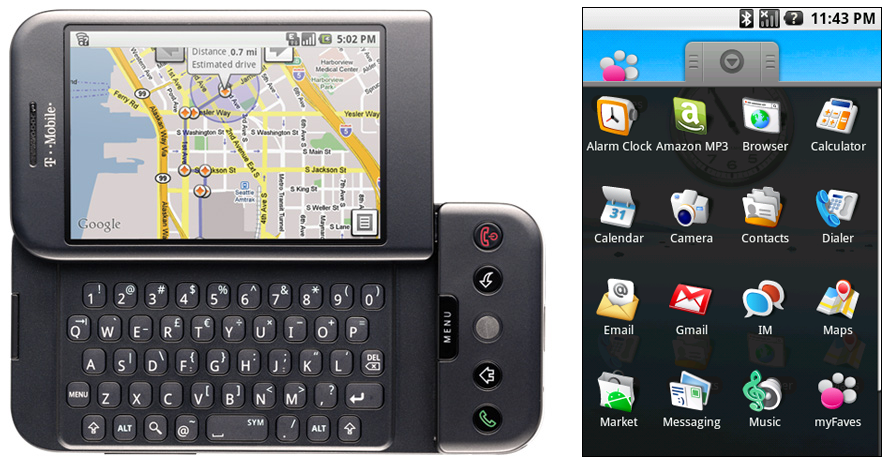
\includegraphics[width=0.8\textwidth]{T-MobileG1Android1menu}
	\caption{The T-Mobile G1 and the Android 1.0 menù}
	\label{2.1:The T-Mobile G1 and the Android 1.0 menù}
\end{figure}

The main characteristic of the OS were and are also now:
\begin{itemize}
	\item The pull-down notification window.
	\item Home screen widgets.
	\item The Android Market.
	\item Google services integration (eg. Gmail).
	\item Wireless connection technologies (eg Wi-Fi and Bluetooth)
\end{itemize}
The success of the first version of the brand new mobile operating system and the open source philosophy guaranteed the fast spread of the Android devices all over the world. In few years Google improved and released many version of the OS and with the help of the market growth Android has become a complete os. 
In the table below there is a brief description of the various distribution of the Android OS at the time of writing of this document.\\
\begin{table}[h]
	%
	\caption{Android versions}
	%
	\label{tab:vers}
	%
	\centering
	%
	\begin{tabular}{lclc}
		%
		\toprule
		%
		\textbf{Name} & \textbf{Version}  & \textbf{Release Date} & \textbf{API Level}\\
		%
		\midrule
		%
		Alpha &	1.0 & September 23, 2008 & 1 \\
		Beta & 1.1 & February 9, 2009 & 2 \\
		Cupcake & 1.5 & April 27, 2009 & 3 \\
		Donut &	1.6 & September 15, 2009 & 4 \\
		Eclair & 2.0 – 2.1 & October 26, 2009 & 5–7 \\
		Froyo & 2.2 – 2.2.3 & May 20, 2010 & 8 \\
		Gingerbread & 2.3 – 2.3.7 & December 6, 2010 & 9–10 \\	
		Honeycomb & 3.0 – 3.2.6 & February 22, 2011 & 11–13 \\
		Ice Cream Sandwich & 4.0 – 4.0.4 & October 18, 2011 & 14–15 \\
		Jelly Bean & 4.1 – 4.3.1 & July 9, 2012 & 16–18 \\
		KitKat & 4.4 – 4.4.4 & October 31, 2013 & 19 \\
		Lollipop & 5.0 – 5.1.1 & November 12, 2014 & 21–22 \\
		Marshmallow & 6.0 – 6.0.1 & October 5, 2015 & 23 \\
		Nougat & 7.0 – 7.1.1 & August 22, 2016 & 24–25 \\
		%
		\bottomrule
		%
	\end{tabular}
	%
\end{table}
 As we can see in \tablename~\ref{tab:vers} there are, currently, 25 level of the Android \textit{API} (Application programming interface
 ) which developers can use to build Android applications. In particular various API levels introduce innovations in the OS but, applications developed using an higher \textit{API level} can not be executed in a device running lower versions of the operating system. This is a second major limitations for the \textit{"Android ecosystem"}, moreover as mentioned before, the Android OS is released under an open source license, which is great for the developer, but which prevents Google to provide updates, in a centralized way, to all devices. For this reason there are currently many active devices running different versions of the mobile OS, as we can check in \tablename~\ref{tab:chart}, which shows, in percentage, the fragmentations of active machines running Android OS.\\
 \begin{table}[h]
 	%
 	\caption{Android OS versions fragmentation}
 	%
 	\label{tab:chart}
 	%
 	
 	%
 	\begin{minipage}{0.5\textwidth}
 		\centering
 		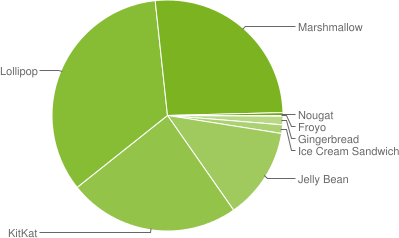
\includegraphics[width=0.9\textwidth]{androidversionchart}
 		 \captionof{figure}{Android OS fragmentation chart}
 		\label{2.2:Android fragmentation chart}
 		
 	\end{minipage}
 ~\hfill~
 \begin{minipage}{0.5 \textwidth}
 	\centering
 	\begin{tabular}{ccc}
 		%
 		\toprule
 		%
 		\textbf{Version}  & \textbf{API Level} & \textbf{Distribution}\\
 		%
 		\midrule
 		%
 		2.2 & 8 & 0.1\% \\
 		2.3.3 - 2.3.7 & 10 & 1.2\% \\
 		4.0.3 - 4.0.4 & 15 & 1.2\% \\
 		4.1.x & 16 & 4.5\% \\
 		4.2.x & 17 & 6.4\% \\
 		4.3 & 18 & 1.9\% \\
 		4.4 & 19 & 24.0\% \\
 		5.0 & 21 & 10.8\% \\
 		5.1 & 22 & 23.2\% \\
 		6.0 & 23 & 26.3\% \\
 		7.0 & 24 & 0.4\% \\
 		%
 		\bottomrule
 		%
 	\end{tabular}
\end{minipage}
 	%
 \end{table}
Data in \tablename~\ref{tab:chart} were collected during a 7-day period ending on December 5, 2016, by Google. Any versions with less than 0.1\% distribution are not shown \cite{devandroiddash}.
\subsection{Structure}
\par
Android is an operating system based on the Linux kernel. The project responsible for developing the Android system is called the \textit{Android Open Source Project (AOSP)} and it lead by Google.
\begin{figure}[h]
	\centering
	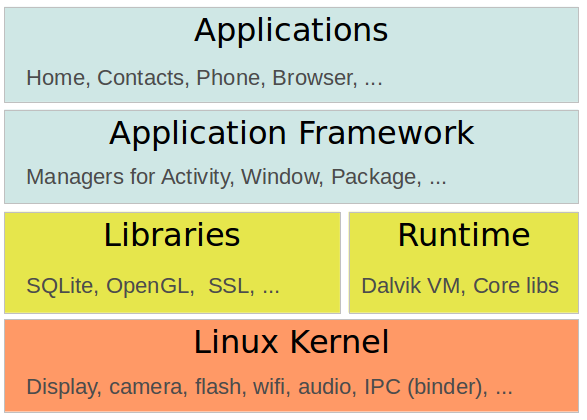
\includegraphics[width=0.8\textwidth]{oslevels}
	\caption{Android OS 4 layers}
	\label{fig:2.3}
\end{figure}

The OS can be divided into the four layers as depicted the \figurename~\ref{fig:2.3}. An Android application developer typically works with the two layers on top to create new Android applications \cite{vogel2016android}.

\paragraph{Linux Kernel} is the most flexible operating system that has ever been created. It can be tuned for a wide range of different systems, running on everything from a radio-controlled model helicopter, to a cell phone, to the majority of the largest supercomputers in the world \cite{hartman2006linux}. This is in practice the communication layer for the underlying hardware.
\paragraph{Runtime and Libraries} \par Runtime is the term used in computer science to designate the software that provides the services necessary for the execution of a program.There are two different \textit{"runtime systems"} which can work with the Android OS:
\begin{itemize}
	\item \textit{Dalvik VM} is an optimized version for low memory devices of the \textit{Java Virtual Machine (JVM)} used in Android 4.4 and earlier version. It is stack based and it works by converting using a \textit{just-in-time (JIT)}, each time an application is executed, Android's \textit{bytecode} into machine code.
	\item \textit{ART (Android Runtime)} introduced with Android 4.4 KitKat. This runtime uses an \textit{AOT (Ahead-of-Time)} approach, with which code is compiled during the installation of an application and then is ready to be executed.
\end{itemize}
\par Standard Android libraries are for many common framework functions, like, graphic rendering, data storage, web browsing. \cite{vogel2016android}. This layer contains also standard \textit{java libraries}.
\paragraph{Application Framework}\label{appframework} is the layer that contains the Android components for the application such as activities, fragments, services and so on. 
\paragraph{Applications} are pieces of software written in \textit{java code} running on top the other layers.

\subsection{Application Framework}
In this section I want to give some details of the application composition and work flow to better understand the subsequent sections in which I will describe the given problem and the proposed solution.\\
As briefly described in \ref{appframework} the Android application framework \textit{("AppFramework")} is the core of the Android \textit{development API}. It contains useful and needed components to build native apps.\\
The main components with which each application is composed are:

\paragraph{Intents} are objects that initiate actions from other app components, either within the same program \textit{(explicit intents)} or through another piece of software on the device \textit{(implicit intents)}.
Acconrding to the official Google's Android for developer documentation, an Intent is a sort of messaging object which can be used to request an action from another application component (eg. activities). There are three fundamental use cases:
\begin{itemize}
	\item Starting an activity: we will see that activities represents a single screen in Android applications, intents allow to start activities by describing them and carrying any necessary data.
	\item Starting a service: I will explain later in deeper details that services are component which performs operations in background. As for the activities, services are initialized through intent and in the same way they describe the service to start and carries any necessary data.
	\item Delivering a broadcast: broadcast is a message that any app can receive. The system delivers various broadcasts for system events, such as when the system boots up or the device starts charging.
\end{itemize}

As already mentioned there are mainly two categories of intents:
\begin{itemize}
	\item explicit intents, used when it is needed to start component within the same application. As the name implies explicit intents call components by using by name (the full \textit{class object} name), for example, it is possible to start a new activity in response to a user action or start a service to download a file in the background.
	\item implicit intents do not name a specific component, but instead declare a general action to perform, which allows a component from another app to handle it. For example, if you want to show the user a location on a map, you can use an implicit intent to request that another capable app show a specified location on a map \cite{devandroidintent}.
\end{itemize}

\begin{figure}[h]
	\centering
	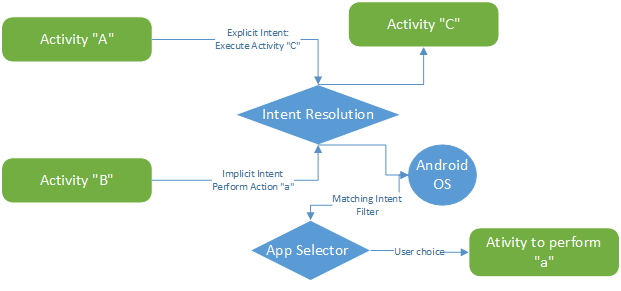
\includegraphics[width=0.9\textwidth]{intentresolution}
	\caption{Intent resolution mechanism}
	\label{fig:2.4}
\end{figure}

The \figurename~\ref{fig:2.4} explains well how an intent is resolved by the OS whether it is implicit or explicit. When an implicit intent needs to be resolved, the OS searches applications which can handle it by means of \textit{intent filters}.A Intent filter specifies the types of intents that an activity, service, or broadcast receiver can respond to. The Android System searches all apps for an intent filter that matches the intent to be resolved. When a match is found, the system starts the matching component, or, if there are more than one, let the user select the preferred action to be performed.

\paragraph{Activities} are one of the fundamental building blocks of apps on the Android platform. They serve as the entry point for a user's interaction with an app, and are also central to how a user navigates within an app. \cite{devandroidactivity}. An activity is the entry point for interacting with the user. It represents a single screen with a user interface \textit{GUI}: in this way activities are containers for other Android's GUI elements (eg. buttons, textviews,...).

\paragraph{Services} is a general-purpose entry point for keeping an app running in the background for all kinds of reasons. It is a component that runs in the background to perform long-running operations or to perform work for remote processes. A service does not provide a user interface \cite{devandroifundamentals}. 

\paragraph{Broadcast Receivers} are components that enable the system to deliver events to the app outside of a regular user flow, allowing the app to respond to system-wide broadcast announcements. Because broadcast receivers are another well-defined entry into the app, the system can deliver broadcasts even to applications that aren't currently running \cite{devandroifundamentals}.

\subsection{Security}\label{androidsecurity}
\par
As described in \ref{briefhist} Android was born to be a good mobile OS and it is mainly for this reason that the system is designed to protect personal and sensible data form malicious guys.\\
Like the rest of the system, Android's security model also takes advantages of the security features offered by the Linux kernel. Linux is a \textit{multiuser OS} and its kernel can isolate user data from one another: one user can not access another user's file unless explicitly granted permission. Android takes advantages of this user isolation, considering each application a different user provided with a dedicated \textit{UID (User ID)} \cite{elenkov2014android} Android in fact, is designed for smartphones that are personal devices and do not need, usually, a multi physical user support.
The most important security techniques adopted by Android are:

	\paragraph{Application Sandboxing} Android automatically assigns a unique \textit{AppID} (Linux UID) when an application is installed and then executed that specific app in a dedicated process as that UID. This technique isolate all the applications at process level and additionally each app has permissions to read/write a specific and dedicated directory.
	
	\paragraph{Permissions} Since application are sandboxed and do not have the rights to read/write date outside them, it is possible to grant additional rights to android applications by explicitly asking them. Those access rights are called \textit{permission}. Applications can request permissions by listing them in a configuration file called \textit{android manifest}. In Android 5.1 and earlier versions permission are inspected and granted at installation time, when the user is alerted with a dialog box in which are listed permissions the application to be installed needs to work properly and when granted cannot be revoked. Starting from android 6.0 permission are asked the first time that an application need them, and when are granted they can be revoked manually in the OS settings for that specific application.
	
		\begin{figure}[h]
		\centering
		\begin{minipage}[c]{.45\textwidth}
			\centering\setlength{\captionmargin}{0pt}%
			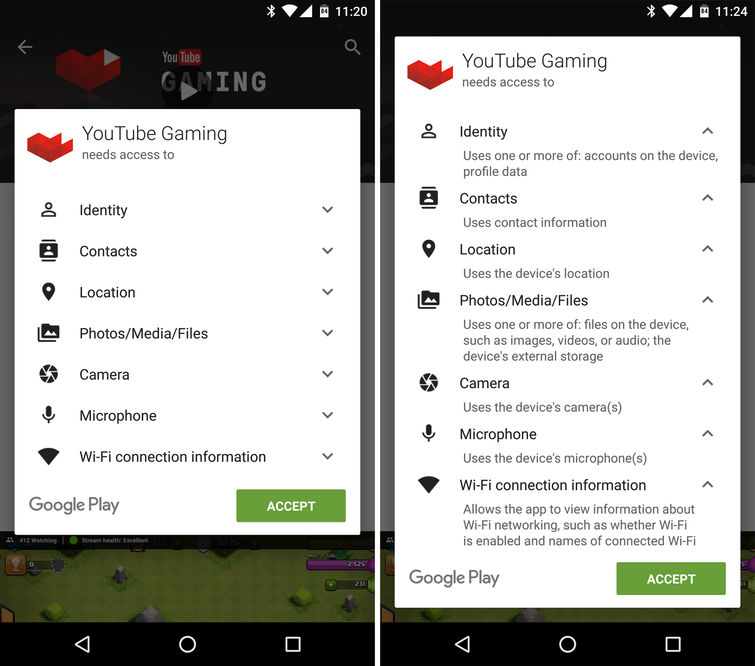
\includegraphics[width=.9\textwidth]{51permissions}
			\caption{Android 5.1- permission example}
		\end{minipage}%
		\hspace{10mm}%
		\begin{minipage}[c]{.45\textwidth}
			\centering\setlength{\captionmargin}{0pt}%
			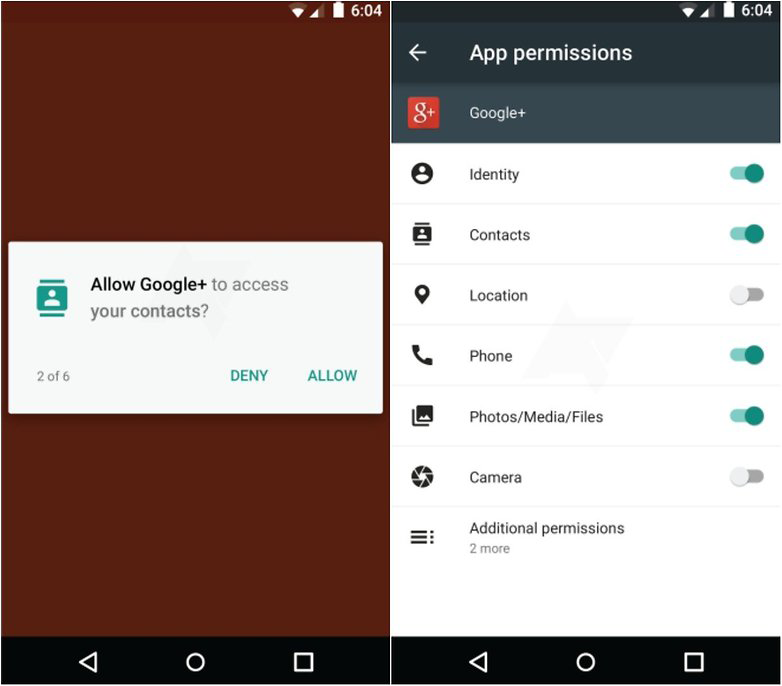
\includegraphics[width=.9\textwidth]{60permissions}
			\caption{Android 6.0+ permission example}
		\end{minipage}
		\caption{Android permission Examples\label{fig:Andorid permission Examples}}
	\end{figure}

	\paragraph{SeLinux} Security Enhanced Linux, is a \textit{mandatory access control (MAC)} system for the Linux operating system. With a MAC the operating system constrains the ability of a subject or initiator to access or generally perform some sort of operation on an object or target. Starting in Android 4.3, SELinux provides a mandatory access control (MAC) umbrella over traditional discretionary \textit{access control (DAC)} environments. For instance, software must typically run as the root user account to write to raw block devices. In a traditional DAC-based Linux environment, if the root user becomes compromised that user can write to every raw block device. However, SELinux can be used to label these devices so the process assigned the root privilege can write to only those specified in the associated policy.
 	In this way, the process cannot overwrite data and system settings outside of the specific raw block device \cite{secure2017android}.

\subsection{Connectivity}\label{connectivity}
\par
As already amply explained previously many Android design choices are due to the fact that it was thought for mobile devices which must have connectivity to intercommunicate among them.\\
With the evolution of various wireless communication technologies, Android devices, nowadays, are equipped whit different kinds of modulus, the most common are:
\begin{itemize}
	\item Wi-Fi
	\item Bluetooth
	\item NFC
	\item Cellular Network
\end{itemize}
The Android Os provide a full library to operate with these technologies and it is possible to integrate in applications the possibility to communicate over these wireless modules.
With the \textit{Android connectivity API} data can be send and received in an efficient way.\\\\
\par
I have only quickly listed some features and possible issues of my source, to have a complete idea it is possible to read all the official Android documentation in \cite{devandroifundamentals}.
 
\section{Distributed System} \label{distsys}
In this section I want to give to the reader some basics about distributed systems, including technical details and examples to make the proposed solution easier to understand.
\subsection{Definition}\label{distdef}
\textit{A distributed system is a collection of independent computers that appears to its users as a single coherent system.}\\
This definition has several important aspects. The first one is that a distributed system consists of components (i.e., computers) that are autonomous. A second aspect is that users (be they people or programs) think they are dealing with a single
system. This means that one way or the other the autonomous components need to collaborate \cite{tanenbaum2010distributed}.\\
\begin{figure}[h]
	\centering
	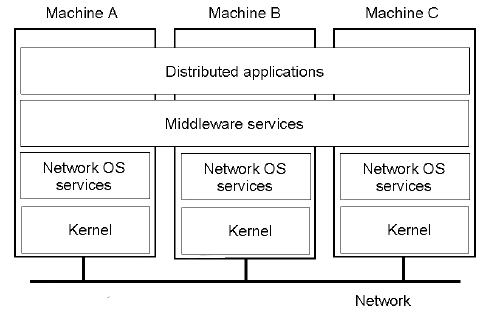
\includegraphics[width=0.8\textwidth]{distributedsystem}
	\caption{Distributed system structure}
	\label{fig:2.8}
\end{figure}
In \figurename~\ref{fig:2.8} it is possible to see how can be structured a distributed system: a the top we have the real distributed application, which is the final interface to be used, under which it is possible to have different combinations of services used to make communicate different machines that may use different operating systems. The real magic is done by the layer called \textit{middleware service} in the picture. A middleware in computer science is a set of software which act as intermediaries between structures and computer programs, allowing them to communicate in spite of the diversity of protocols or running OSs.

\subsection{Challenges} \label{chall}
There are many challenges in distributed systems field: distributed applications are often really complex and easily exposed to physical and technical failures because of their nature. Major challenges and property to be considered when developing a system of this kind are:

\begin{figure}[h]
	\centering
	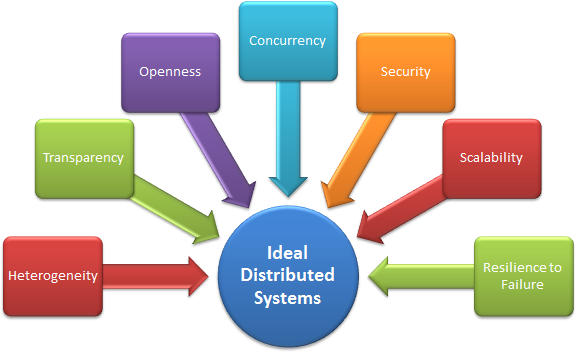
\includegraphics[width=0.8\textwidth]{challengesdistributedsystems}
	\caption{Distributed system challenges}
	\label{fig:2.9}
\end{figure} 

\begin{itemize}
	\item Heterogeneity, is a major challenge because there are many different component to be considered, distributed systems may be developed for example for different hardware, networks, operating systems and programming languages.
	\item Openness, determines whether a system can be extended and reimplemented in various ways, so distributed systems should use standards as much as possible. Developers should always choose the simplest ways during design and implementation phases.
	\item Security, is crucial in many areas of computer science and specially in distributed systems, where data are exchanged by a several number of machines.
	\item Scalability, is the ability to easily increase the size of the system in terms of users/resources and geographic
	span.
	\item Failure handling, is important because having different components working together to a common goal means that distributed system can fail in many ways. This raises some issue: it would be nice id distributed systems can detect, mask and tolerate failures.
	\item Concurrency in distributed systems is a matter of
	fact, access to shared resources (information or services)
	must be carefully synchronized.
	\item Transparency level are listed in \tablename~\ref{tab:transparency}
\end{itemize}

	\begin{table}[h]
		%
		\caption{Transparency levels}
		%
		\label{tab:transparency}
		%
		\centering
		%
		\begin{tabular}{lp{0.75\textwidth}}
			%
			\toprule
			%
			\textbf{Transparency} & \textbf{Description}\\
			%
			\midrule
	%
			Access & Hide differences in data representation and how a resource is accessed\\
			Location & Hide where a resource is located\\
			Migration & Hide that a resource may move to another location\\
			Relocation & Hide that a resource may be moved to another location while in use\\
			Replication & Hide that a resource may be shared by several competitive users\\
			Concurrency & Hide that a resource may be shared by several competitive users\\
			Failure & Hide the failure and recovery of a resource\\
			Persistence & Hide whether a (software) resource is in memory or on disk\\
			%
			\bottomrule
			%
		\end{tabular}
		%
	\end{table}

\subsection{Comunication Model}
\par
There are, in distributed system literature, some well known techniques to let communicate machines, programs and components. Each of the methods described later exploits the network protocols by acting as a middleware: they use and mask lower layer protocols to provide ready to use communication services.

\paragraph{Remote procedure call (RPC)} is a paradigm in which a client process invokes a remotely located procedure (a server process), the remote procedure executes and sends the response back to the client \cite{Jerome2009Principles}.
\begin{figure}[h]
	\centering
	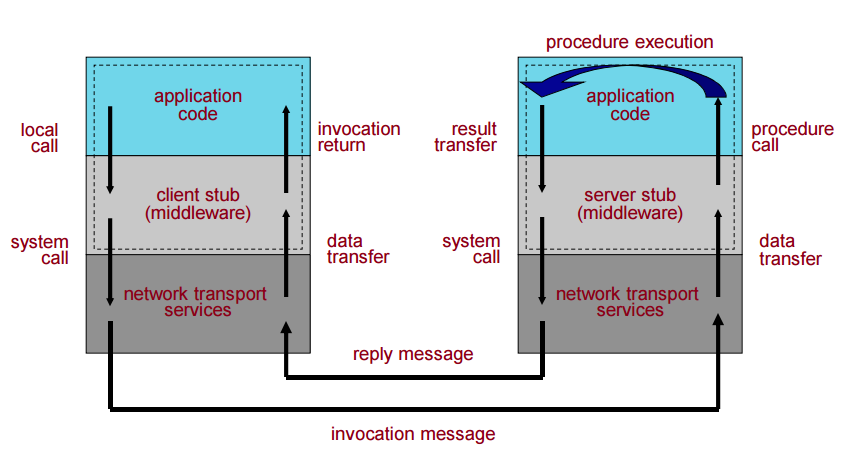
\includegraphics[width=0.8\textwidth]{rpc}
	\caption{RPC in detail}
	\label{fig:2.10}
\end{figure} 
As described in \figurename~\ref{fig:2.10} RPC provides the localization of the code to be executed exploiting the network transport services, create a message which can be serialized and transferred over a standard network protocol and then provides methods to de-serialize the message and convert in into a standard local procedure call in the receiver machine. Very important in this mechanism is the concept of \textit{ILD} (Interface definition language) which raises the level of abstraction of the service by separating the interface from its implementation: in this way RPC can be language independent by generating automatic translations from IDL to target language.  
\paragraph{Remote method invocation (RMI)} exploits the same idea of RPC but with different programming constructs: it is designed to let communicate object oriented (OO) programming languages.
\begin{figure}[h]
	\centering
	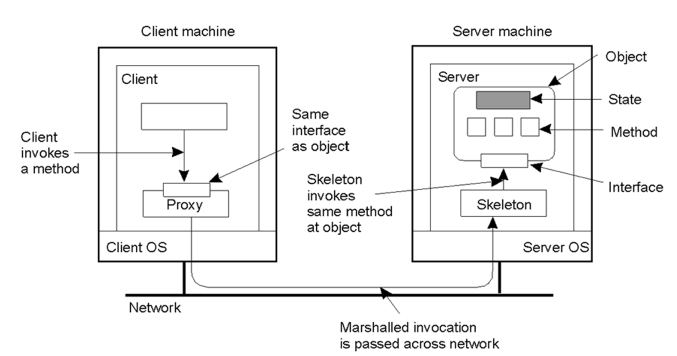
\includegraphics[width=0.8\textwidth]{rmi}
	\caption{RMI in detail}
	\label{fig:2.11}
\end{figure} 
The \figurename~\ref{fig:2.11} shows in detail how RMI is supposed to work. Like RPC, RMI uses an IDL which is designed to support OO programming languages features such as inheritance and exception handling.
\paragraph{Message oriented} communication is a style based and centered on the notion of simple messages and events.The most straightforward example of it is \textit{message passing}. Typically message passing is implemented directly on the network sublayers (eg. sockets). Message passing differs from conventional programming where a process, subroutine, or function is directly invoked by name. 
\begin{table}[h]
	%
	\caption{Comparison between communication models}
	%
	\label{tab:comp}
	%
	\centering
	%
	\begin{tabular}{p{0.45\textwidth}p{0.45\textwidth}}
		%
		\toprule
		%
		\textbf{RPC/RMI} & \textbf{Message Oriented} \\
		%
		\midrule
		%
		& \\
	      \begin{minipage}[t]{0.45\textwidth}
	     	\begin{itemize}
	     		\item natural programming abstractions
	     		\item point to point communication
	     		\item designed for synchronous communication
	     		\item high coupling between the caller and the callee
	     	\end{itemize}
	     \end{minipage} &  \begin{minipage}[t]{0.45\textwidth}
	     \begin{itemize}
	     	\item centered around the notion of message/event
	     	\item multipoint support
	     	\item usually asynchronous
	     	\item high level of decoupling
	     \end{itemize}
     \end{minipage} \\
  & \\
		
		%
		\bottomrule
		%
	\end{tabular}
	%
\end{table}
In \tablename~\ref{tab:comp} are shown the most significant differences between RPC/RMI approach and message communication models. Moreover there are some implementation of message passing at middleware layer like \textit{publish-subscribe} which is further explained in the following paragraph.

\subsection{Architectures}
\par
There are actually many different kinds of distributed systems which can be classified by means of their architecture composition.
\paragraph{Client-Server} is the most common architecture in computer systems, there are many variants depending on the internal division of its components but it has a common separation of duties. Server side components are passive and wait for clients invocations.Client computers provide an interface to allow a computer user to request services of the server and to display the results it returns. Servers wait for requests to arrive from clients and then respond to them. Ideally, a server provides a standardized transparent interface to clients so that clients need not be aware of the specifics of the system (i.e., the hardware and software) that is providing the service. The communication adopted by these kind of systems is message oriented or through RPC.
\begin{figure}[h]
	\centering
	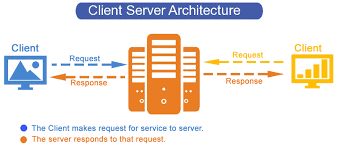
\includegraphics[width=0.8\textwidth]{clientserver}
	\caption{Client server architecture}
	\label{fig:2.12}
\end{figure} 
\paragraph{Peer-to-Peer (P2P)} is a fully distributed architecture which in contrast to client-server has not a centralized service provider. Peers are both clients and servers themselves, P2P promotes sharing of resources and services trough direct exchange between peers. Compared to a centralized client-server architecture a P2P net scales better and typically does not have a single point of failure. 
\begin{figure}[h]
	\centering
	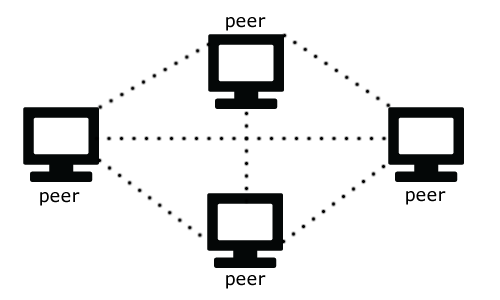
\includegraphics[width=0.8\textwidth]{p2p}
	\caption{P2P architecture}
	\label{fig:2.13}
\end{figure} 
\paragraph{REST style} Representational State Transfer (REST) is a style of architecture based on a set of principles that describe how networked resources are defined and addressed.An application or architecture considered RESTful or REST-style is characterized by:
\begin{itemize}
	\item state and functionality are divided into distributed resources,
	\item every resource is uniquely addressable using a uniform and minimal set of commands (typically using HTTP commands of GET, POST, PUT, or DELETE over the Internet),
	\item the protocol is client/server, stateless, layered, and supports caching.
\end{itemize}



\paragraph{Event based} is an architecture in which components collaborate by exchanging information about occurring events. In particular components in the net can \textit{publish} notifications about the events they observe or \textins{subscribe} to events they are interested to be notified about. This architecture can be fully distributed with all the same nodes or can have some semi-centralized nodes which are specialized in computing events or routing messages. Communication is, in this case, purely message based asynchronous and multicast. 
\begin{figure}[h]
	\centering
	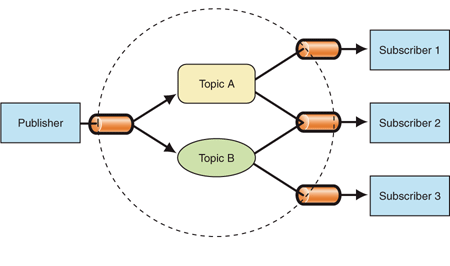
\includegraphics[width=0.8\textwidth]{publishsubscribe}
	\caption{Publish-subscribe architecture}
	\label{fig:2.14}
\end{figure} \\\\\\

\subsection{Naming}
%descrivere problemi di naming e 0 conf
Naming is one of the major issues when building distributed systems, in fact, it is often impossible to know a priori, exactly the addresses and port services of all the components in a distributed network, especially when the system allows dynamic connections and disconnections. It is important therefore, to adopt a naming model or service, to automatize components discovery and connections, when running a distributed system. To understand how naming models e solvers work it is important to introduce some naming concepts in the distributed systems paradigm.\\
In distributed systems names are used to identify a wide variety of resources such as computers, hosts, files, services as well as users. Names are usually accessed by an \textit{access point} which is a special entity characterized by an \textit{address}. Addresses are just special names which can be used by communications protocol to connect different machines. For this reason it is important to know access point addresses because otherwise it would be impossible to connect components. Dynamic systems let components change access points frequently, so having \textit{location-independent} names is much more convenient than known static addresses which can change during system execution. \textit{Identifiers} such that they never change during the lifetime of an entity, are unique, and can not be exchanged between different entities. In this way, using identifiers, it is possible to split the naming problem in two: mapping a name to the entity and then locating the entity itself.
Naming schemes are the solution to the first problem, and the most used ones are:
\begin{itemize}
	\item \textit{Flat naming}, or unstructured, are simple identifiers represented by random strings of bits.An important property of such a name is that it does not contain any information whatsoever on how to locate the	access point of its associated entity \cite{tanenbaum2010distributed}.
	\item \textit{Structured naming} are composed from simple, human-readable names, not only file naming,but also host naming on the Internet follow this approach,in fact, flat names are good for machines, but are generally not very convenient for humans to use \cite{tanenbaum2010distributed}.
	\item \textit{Attribute based naming} is a way to describe an entity in terms of \textit{(attribute, value)}
	pairs. Flat and structured names generally provide a unique and location-independent
	way of referring to entities. Moreover, structured names have been partly
	designed to provide a human-friendly way to name entities so that they can be
	conveniently accessed. In most cases, it is assumed that the name refers to only a
	single entity. However, location independence and human friendliness are not the
	only criterion for naming entities \cite{tanenbaum2010distributed}. Using attribute based naming is possible to give more information about entities or services to be found.
\end{itemize}
The solution to the second problem is called \textit{name resolution}. Name resolution in the process of obtaining the address of a valid access point of an entity having its name. Name resolution services highly depends of the naming model adopted by a system.\\
For sake of brevity here are not reported any detail of name resolution systems, but only basic naming notions to understand author's design choices in solving the thesis problem. 


\section{Liquid computing}\label{liquid computing}
\subsection{Definition}
The term was coined for Apple's liquid computing feature and  refers to a style of work-flow interaction of applications and computing services across multiple devices, such as computers, smartphones, and tablets.\\
In a liquid computing approach, a person might work on a task on one device, then go to another device that detects the task in progress at the first device and offer to take over that task.
In other terms liquid computation is a sort of what is called \textit{ubiquitous computing} which is a model of man-machine interaction in which information elaboration is integrated in everyday objects.
\subsection{Examples}
There are some implementation of this concept in mobile computer science, the most significant are:
\begin{itemize}
	\item Apple continuity, is a system, developed by Apple, with which a user can initiate a task on one device and end the task on another. For example it is possible to answer a call with a computer without using the phone.
	\item Google chrome and Gmail, developed by Google, allow users to surf the web and to write email on every available device as if they were using a single device. By registering a Google account chrome can save the navigation history of the user and show it on any logged device. In the same way Gmail saves automatically emails and for example is possible to start writing an email on a desktop pc and then completing and sending that email on a smartphone.
	\item Microsoft One Drive sync is a system, developed by microsoft to allow users to synchronize file and settings among their devices like desktops, notebooks smartphones and so on.
\end{itemize}





%
% ------------------------------------------------------------------------ %6
%
% ------------------------------------------------------------------------ %
% !TEX encoding = UTF-8 Unicode
% !TEX TS-program = pdflatex
% !TEX root = ../Tesi.tex
% !TeX spellcheck = en_US
% ------------------------------------------------------------------------ %
%
% ------------------------------------------------------------------------ %
% 	Problem analysis and proposed solution
% ------------------------------------------------------------------------ %
%
\chapter{Problem Analysis}
%
\label{cap:probanalysis}
%
% ------------------------------------------------------------------------ %
%

In this chapter the specific problems of this work will be detailed and analyzed, explaining what are the limits and the constraints the challenge has. The chapter starts with a brief recap, followed by the proper definition of what I faced, while in the last part there is a list of constraints my architecture will have fulfilled in order to have a universal and functional solution.
  

\section{Contextualization} \label{facedProblem}
As already explained introducing this thesis work in \ref{motivation}, I studied in deep the Android operating system to find, and later implement a concrete solution, to the problem I will define and describe in dept in this section. All the work done by me is focused on Android because every mobile operating system is different to each other and has proprietary working mechanism which have to be studied separately. Since there are many more Android devices than any other mobile OS, and Android is an open source software and there is no need to buy development licenses or proprietary hardware or software like using for example Apple systems, I decided to work with it, even if by studying another mobile OS and implementing the same concepts of my solution it is certainly possible to achieve the same result i got by working only with Android. 
In the previous chapter, number \ref{cap:statoarte}, I have defined Android OS working mechanism and components, pointing out the main focus on intent generation and resolution mechanism. I have then defined in deep what a distributed system is and should be, explaining connection mechanism architectures and properties.\\ 
The Android OS is a centralized operating system designed for a single physical user, to be used on personal mobile devices such as smartphones and tablets. The result of this Google's ideas is that in contemporary society there is a wide spread of Android devices, which now have computing capacity comparable to normal desktops and notebooks. Many people have multiple devices which they use separately: typically they use smartphones for calls and  work emails and maybe tablets to easily surf the Internet and play games, but what they can not do is use them together to perform a common task easily. Android, in fact, has not been thought to build a real distributed system, the networking functionalities are designed to exchange messages, and to replace standard personal computers in some task as indeed sending emails.
The result is a non collaborative confused cloud of devices, which are connected to the net, but are not really connected themselves to cooperate. Solutions are often partial or proprietary and closed, even if some useful solutions exist.\\
The idea is let android devices collaborate and cooperate in a \textit{Liquid environment} like the one presented in section \ref{liquid computing}. The fundamental requirement is the implementation of an android service, able to build and maintain a distributed net of android devices over a Wi-Fi LAN (Local Area Network), and then let one, or more devices in that net generate Android intents and distribute them one, or more, of the other devices involved. Thus in this chapter I am considering only Android devices that can be connected in a WiFi LAN.\\
After this brief recap of what has been said about the Android OS and distributed systems in the state of the art chapter, here I am trying to define with more precision the problem I am going to face: which its constraints and its possible goals are.

\section{Considered Devices}
As anticipated above, I am going to take into account only devices that can be somehow connected to a LAN, but as described in \ref{connectivity} Android devices are built to be connected to the Internet and most of them comes with a WiFi chip integrated. Another \textit{"little relaxation"} I want to do is linked to the variety of Android OS versions. I want to take into account only devices updated to at least version 4.4 (API level 19). This is due to the fact that starting from Android KitKat (4.4 version) Google brought some important improvements  to the libraries of the framework and in addition, according to the \tablename~\ref{tab:chart}, with this choice it is possible to cover the 84\% of the active Android devices.\\
Having done these clarifications, now I am defining the problem.

\section{Definition} \label{problemdefinition}
\textit{How can we transform a standard mobile OS into a distributed version of it?} This is the general question I want to give an answer in this work.
As already said the Android OS is a pretty closed system itself, the intent resolution mechanism shows how it is difficult to let communicate various components inside a single device. On the other hand it is equally true that Android devices are real powerful modern computers and would be great if somehow it could be possible to have a device able to detect other devices in a LAN send data and task to perform in a transparent way and then get back, if necessary, result or data. Let me be more concrete, often in a home environment there are several android devices, with a distributed intent resolution mechanism it would be possible for example to take a photo from one device with the camera of another one, to generate an intent to open a file on a group of devices simultaneously, to play a video remotely and so on, only by generating intents and then send them to the distributed net. \textit{How can we let multiple android devices act as a single big distributed system?} This is the question that my thesis is trying to answer. My work is a concrete solution, it is about defining and creating a method to distribute android intents from one device to other in a LAN and then let the OS act as usual to manage and resolve them.\\
So I am trying to let different android devices talk by means of distributing intents using  well known architecture: a master component, let me call it \textit{distributed intent generator} acting as client, and a slave component \textit{distributed intent solver} acting as a server. The two components i will realize will be common Android background services registered on the WiFi LAN. Both of these components will result in android applications so that a single device could be used to control others or to be controlled.\\
In \figurename~\ref{fig:3.1} is presented how such a system should work once the net is up. The distributed system in figure is a simplification of what the middleware for distributing intents will do. The architecture will communicate using standard android networking messages that are build on top standard protocols of the ISO/OSI stack.
 
\begin{figure}[h]
	\centering
	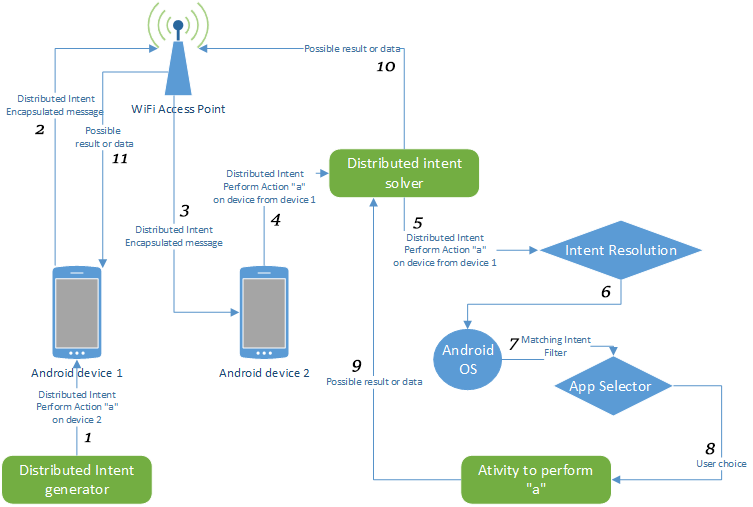
\includegraphics[width=.95\textwidth]{scheme}
	\caption{Distributed intent resolution}
	\label{fig:3.1}
\end{figure}

The important point is having a message with a well defined content: it is what the two parts must write and read, so it has to be clear for machines, must be compliant with all the requests of \textit{M2M (Machine-to-Machine) communication}. This type of communications is a constraint of my work and are explained in the next section \ref{problemconstraints}.Another important point is let the Android OS work as it is designed for, the main aim of this thesis work is to build a middleware to let distribute native Android intents over the network. This is a new approach to this problem in fact, there are yet some android applications which let the user send stream or data to other devices in a LAN but, with specialized and ad hoc built messages within the same application context, using a mechanism really close to explicit intent resolution. My middleware is supposed to address the problem using a more general approach and a mechanism equal to implicit intent resolution. What I'm doing is create a system to spread any kind of implicit intent and let the OS react as usual to perform the required action.
It is not even marginal the choice of the type of network to be used in such a system. Android devices are in fact, usually, mobile devices, and for this reason they can be easily moved from one place to another, so the network must take into account this property dynamically react to continuous changes.\\
Next sections will properly define all the constraints of the given problem and propose a solution that fulfills them all.
\section{Probelm scenarios}
As already anticipated with the definition of the problem,  the aim of this thesis is to give the feeling, to users, that they are working with multiple Android devices as if they were one single distributed operating system. I want to analyze some problematic scenarios an then in the next chapter of the thesis provide, if possible a solution to each specific case.

\subsection{Background working middleware}\label{middlewarescenario}

\begin{figure}[h]
	\centering
	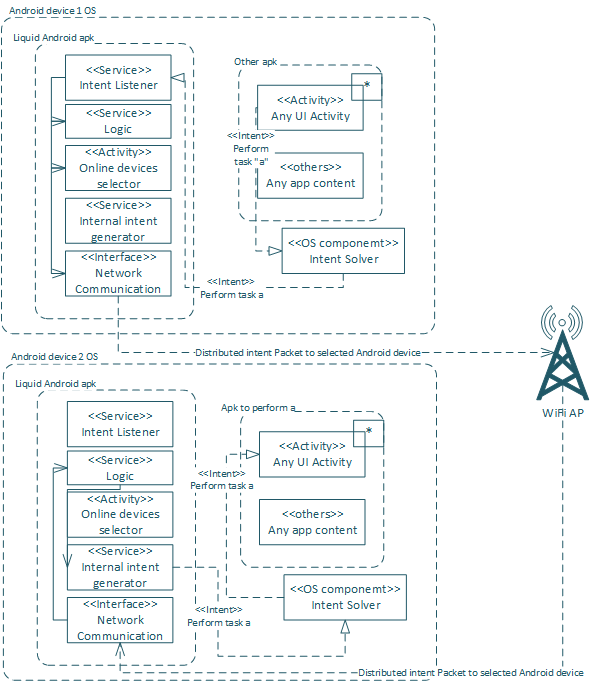
\includegraphics[width=.85\textwidth]{scenario1}
	\caption{Liquid Android working as stand alone middleware APK}
	\label{fig:3.2}
\end{figure}
 

In the best case, the result to be achieved would be a single Android APK, to be installed on devices as background bunch of services acting as a middleware. Liquid Android services which providing a communication interface can listen distributed events invocations and react to them automatically. The middleware may intercept local intents, find online devices in the distributed network, let the user select on which of them execute the task and send the intent to the selected remote Android device.\\
The \figurename~\ref{fig:3.2} shows a possible UML component diagram of the Liquid Android middleware, the scheme points out the interactions between the Liquid Android application (APK) and other possible applications installed on the device. The group of services intercepts the local intent, created by a different application in the same device, let the user of the system select on which available device execute the task, build and spread the the distributed intent message on the LAN, and when the message arrives at the other device the middleware transform the received message in a local intent to be resolved as usual by the operating system.\\
I want to provide a simple but concrete example to be more precise, every Android OS version comes with a web browser installed as an APK. When an application needs to open a URL with a browser generate an intent to perform such an action, with a middleware as described above it would be possible to click on the URL on a first device and to open the link in a second device having only installed the Liquid Android APK on both devices.

\subsection{Development API}\label{devAPI} A second interesting scenario is one in which the Liquid Android middleware could become a ready to use \textit{application programming interface (API)}. By abstracting the underlying implementation and only exposing objects or actions the developer needs, an API reduces the cognitive load on a programmer. By developing the middleware as an API is it possible to give to Android programmers a library to implement easily and faster, native Android distributed applications. The API implemented could be integrated during the development of such applications like other Android libraries to generate one single APK containing also Liquid Android components. For these purposes it is necessary to produce accurate documentation for developer who could use the Liquid Android API.\\
As already done for the previous case, let me make an example.
\begin{figure}[h]
	\centering
	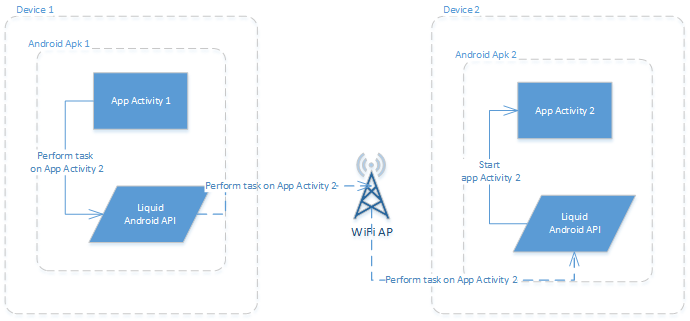
\includegraphics[width=.9\textwidth]{esempio2}
	\caption{Liquid Android API working example}
	\label{fig:3.4}
\end{figure}
In \figurename~\ref{fig:3.4} there is a scheme showing how the middleware could be used to build two different applications with two different packages (apk) including both the Liquid Android API which let them communicate by sending Android intent generated by \textit{Android Apk 1} and then received by \textit{Android Apk 2} installed respectively on two different devices.

\subsection{Data management}
\begin{figure}[h]
	\centering
	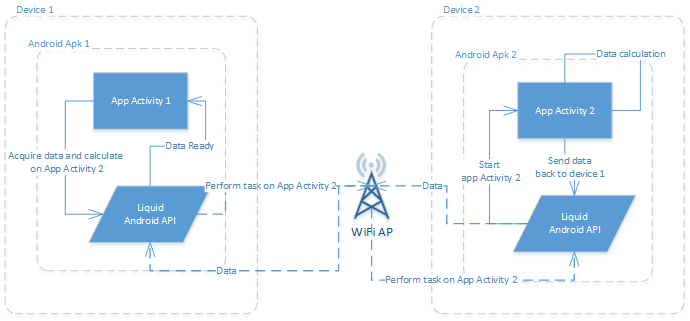
\includegraphics[width=.9\textwidth]{scenario3}
	\caption{Liquid Android API data management example}
	\label{fig:3.5}
\end{figure}
Last interesting scenario tu study is the data management problem in using such a system. This is a different type of scenario because it involves both previous scenarios. Having a distributed system always raises the problem of distributed data and data consistency. The middleware to be implemented must consider also the possibility to be used to build distributed Android applications in which data are generated somewhere by one device and then they need to be processed for a result by another one. A simple, but not trivial, example could be the case of a distributed calculator. A device acquires data and sends them to another one to be processed and then ask to that device the results. In the Android environment there is not the concept of distributed file system, so data involved in such an application must be considered and efficiently exchanged between devices.


\section{Constraints} \label{problemconstraints}
In this section I would like to list a set of  constraints for the defined problem, that become requirements that the solution must meet. The section should be divided into two parts, the first for the requirements of the network, the second for the ones of the Android distributed intent generator and solver. The two sections are actually closely related so here I preferred to keep the two parts together, analyzing the entire middleware structure.\\ 
Here is the list:

\begin{itemize}
	\item \textit{M2M communication:} M2M communication is defined as a communication in which the two interlocutors are not humans. It is a communication completely handled by machines and computers \cite{cha2009trust}. It can be considered one of the fundamental enabling technologies of this thesis work, it permits object to communicate without humans being involved. In This type of communication the reader of the content is a computer, in this case are Android devices. The content of the messages must be well formed, the middleware must react properly to the event of receiving a distributed intent. So a clear, defined syntax with a well fixed structure  must be set in order to make everything understandable to a computer.
	
	\item \textit{Transparent:} As already widely discussed a middleware is those which do the \textit{magic}. The proposed solution is intended to be transparent to the Android OS and let it work as usual in resolving implicit intents whether they are distributed or not. Moreover as discussed in the chapter \ref{cap:statoarte}, to be more precise in \tablename~\ref{tab:transparency}, a distributed system must be transparent at many level, in this case the middleware must act as resources manager and efficiently mask resources access and location.
	
	
	\item \textit{Lightweight:} Another constraint to my system is the fact that whatever system I choose to be the solution it must be lightweight. This is needed because my system will work on a WiFi LAN. Messages must be encapsulated, serialized from one device and transferred in another one to be deserialized and analyzed to be executed. Messages must be as easy as they can because they are very frequent in such a system.
	
	\item \textit{Modular:} The implementation of the solution must be modular, this is due to the fact that this middleware is intended to be used as is but also to implement easily other kind of native Android distributed system application. Having a modular structure facilitates the specialization of its component and make all the middleware more readable and easy to use. In this way \text{Liquid Android} can be the substructure of other works.
	
	\item \textit{Extensible:} the implemented solution must meet canonical programming principles Extendability is one of the most important properties to take into account when building a computer system, especially when developing a middleware. Liquid Android modules have to be extensible to be improved or adapted to different purposes.
		
	\item \textit{Secure:} Liquid Android middleware must meet standard Android security design principles as described in \ref{androidsecurity}. The implementation must not exceed the limits imposed by the OS, I do not want to break the Android permission scheme and authorization model by \textit{rooting} the operating system, a process with which is possible to perform action as the administrator in Android environment. Rooting Android devices let application overcome the boundaries of standard applications, by letting them read and write data from all the OS. Moreover the middleware operates on mobile devices which usually contains and can manage many sensible and personal data, communications between these devices must be as secure as possible to limit security threats.
	
	\item \textit{Consistent:} Data and accessed resources involved in the system must meet consistency requirements. When developing distributed systems consistency is one of the main issue. The implemented solution must take into account data produced during the use of the system and make them consistent according to a chosen consistency model.
	
	\item \textit{Scalable:} the system to be implemented has not a fixed number of devices involved in. The chosen network architecture must be able to react according to the changes. Android devices are free to join or leave the network any time, and the system should be able to detect and maintain a dynamic network. Scalability is, in fact, the capability of a system, network, or process to handle a growing amount of work, or its potential to be enlarged in order to accommodate that growth \cite{bondi2000characteristics}. 
	
	\item \textit{Concurrent:} another important aspect of distributed systems is concurrency. Concurrency is the decomposability property of a program, algorithm, or problem into order-independent or partially-ordered components or units \cite{lamport1978time}. The implementation of the services must ensure this property to the system. The middleware has to have the capability to handle different requests at the same time and execute task in more than one device simultaneously.
	
\end{itemize}
The listed requirements, as already told in some of them, are, sometimes, general, in the sense that they have to be respected for the final product: a global and complete structure that starts from the construction of the network architecture arrives to the user's interaction activities on Android devices. This is because the problem I am facing is very big and complex, and it is transversal to the existing technologies, so the whole system must work properly. Keeping in mind what I have just stated, some of these constraints become fundamental requirements that my system must meet. My work has to be clear for developers to be used for further implementations of native Android distributed systems, but even if it can be less clear to an average user it must be usable to those wishing to try distributed intents with their own devices in a home LAN.

\bigskip
\bigskip
\bigskip
\bigskip
\bigskip
\bigskip
\par
In the next chapter I am presenting my idea, the \textit{Liquid Android} middleware, the so called solution to the given problem, explaining what I have done, my considerations about the situation here faced.

%
% -----------------------------END------------------------------------- %
%
% ------------------------------------------------------------------------ %
% !TEX encoding = UTF-8 Unicode
% !TEX TS-program = pdflatex
% !TEX root = ../Tesi.tex
% !TeX spellcheck = en_US
% ------------------------------------------------------------------------ %
%
% ------------------------------------------------------------------------ %
% 	PROPOSED SOLUTION
% ------------------------------------------------------------------------ %
%
\chapter{Proposed Solution}
%
\label{cap:proposedsolution}
%
% ------------------------------------------------------------------------ %
%
\par In this chapter the development of the solution will be reported step by step, with a full use case. The chapter starts with a list of similar solutions already developed, highlighting the differences between them and my thesis work. The remaining part is composed of tree mains sections: the first explains the choice of the network, the architecture, the naming service, etc. It lays the foundations for the second part: the definition of the Liquid Android middleware, or better the structure of what will do the magic: intercept, encapsulate, spread, and generate distributed intents in the network so made. The two parts are closely related, therefore their relation was taken into account when I made my choice.\\
The real implementation of the valid solution is left for the next chapter.
%

\section{Existing Solutions }
Android distributed systems already exists as specific purposes application to be installed on multiple devices, what it is different to the aim of this thesis work is that these application are closed source projects that can not be reused to build other purposes systems and there is not a coherent framework, library or API to be used to easily build such systems.
I want to give some examples pointing out the nice features have this native distributed Android systems.
\subsection{Boincoid and HTC Power to Give}
Boincoid and HTC Power to Give are Android application which aim is  to exploit Android devices computation power to contribute to scientific discoveries by doing some task. The common idea is to have an Android distributed supercomputer which can handle heavy task and compute tons of data for larger purposes.\\
BOINC is an open-source software platform for computing using volunteered resources \cite{boinc2017open}. It is a program that lets you donate your idle computer time to science projects. Boincoid is a port of the BOINC platform to the Android operating system. The result is an Android BOINC client that behaves exactly like the original one.\\
HTC Power to give is very similar to Boincoid, it is a \textit{CSR (Corporate Social Responsibility)} initiative from HTC that has been jointly developed with Dr. David Anderson at University of California, Berkeley. Using the HTC Power To Give, owners of Android OS smartphones can choose to ‘give back’ by supporting key research projects around the world. Scientific research often requires a vast amount of processing power for data modeling and analysis. HTC Power To Give, supported by the world’s largest single distributed volunteer computing platform BOINC, lets users donate their unused smartphone computing power to science programmes across diverse fields as astronomy, environment, medicine and physics \cite{htc2017power}.
 
\subsection{Plex for Android}
Plex platform is a great, maybe the best, media content streaming distributed system platform. It is mainly composed of two components, the media server, and a client with which enjoy the contents.
\begin{figure}[h]
	\centering
	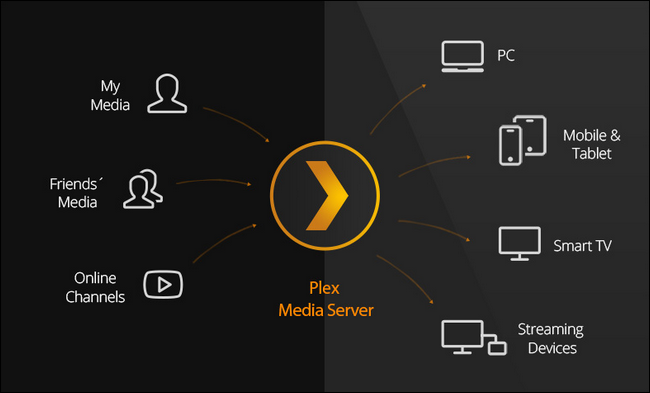
\includegraphics[width=.8\textwidth]{plex}
	\caption{Plex Platform}
	\label{fig:4.1}
\end{figure}
The Plex Media Server either running on Windows, macOS, Linux, FreeBSD or a NAS which organizes audio (music) and visual (photos and videos) content from personal media libraries and streams it to their player counterparts.
The players can either be the Plex Apps available for mobile devices, smart TVs, and streaming boxes, or the web UI of the Plex Media Server called Plex Web App, or the old Plex player called Plex Home Theater.\\
In particular Plex for Android application can connect to the media server to play its content and in addition it can search for Plex players in a LAN and send streamed content such as videos, movies or photo, to another player that can be also an Android device. In this way the Android Plex application client can behave like the Liquid Android system i want to develop. It can send a sort of \textit{Android intent}, to reproduce a media, from one device to another, and then it can send commands such as pause, rewind, forward and so on. The limits of such a system are that it is possible to send, and play, only multimedia contents, and only to devices which have the Plex app activity in foreground on the device.

\subsection{Goolgle Home and Cast API}
Google itself provides an application to control and send contents form an Android device, to some special devices in home network. \textit{Google Home} is an Android application which can find, setup, manage and control, Google's home devices like the \textit{Google Chromecast}. In this way is easy to setup and control and Android distributed system in which user can sent multimedia contents and command to the Google Home devices in the LAN. For these reason Google provides a development library, included in the Android framework, called \textit{Cast API} with which it is easy, for a developer, to build applications that can send multimedia streams to other Google devices specifically built for these purposes.\\
Also in this case the limitation is the kind of content, only multimedia, and also the type of devices involved which are limited number of special purposes devices.

\subsection{DroidMote and Remote control systems }
If we consider the possibility to control remote devices in a LAN, there are actually many different kind of applications that can do that also in an Android environment.
DroidMote is probably the most complete application to control remotely an Android device from another one. It is composed by two parts, the server, to be installed in the device to be controlled, and the client, to be installed in the one which controls. With this application is possible to control entirely the device running the server component: is it possible to open applications, perform tasks, open system settings and so on.\\
These kind of systems are capable to generate local intents in remote devices over a LAN but in a completely different way from I want to develop the solution to the given problem. In this case the \textit{controller} is explicitly controlling the remote device as it is using only the \textit{controlled} one. These systems are solution only to the problem of remote control, they can not exploit distributed Android devices computation power, in fact in an environment like this Android devices are not cooperating to perform task but one of them is only controlling another one.
\section{General Idea}
\section{Network Architecture}


%
% -----------------------------END--------------------------------- %
%
% ------------------------------------------------------------------------ %
% !TEX encoding = UTF-8 Unicode
% !TEX TS-program = pdflatex
% !TEX root = ../Tesi.tex
% !TeX spellcheck = en_US
% ------------------------------------------------------------------------ %
%
% ------------------------------------------------------------------------ %
% 	CONCLUSIONI
% ------------------------------------------------------------------------ %
%
\chapter{Case Study}
%
\label{cap:proofofconcept}
%
% ------------------------------------------------------------------------%
In this chapter I will describe the real implementation of the system, which is the real solution of the problem faced by this thesis work: how it is possible to extend a mobile operating system, in this case Android, with distributed OS functionalities.\\
This chapter is mainly composed of three parts: the first one is a generic information
section in which the proof of concept is explained in terms of technologies
used, requirements to meet, goals and various technicalities. The second one
is the report of the implementation and development of the application, with
choices and descriptions of what has been done. The third part is a working demo of the
just described system, with live working test cases. It contains screenshots of the
application while it is running and a complete description to explain each case
step by step.
\section{Conception}
As already specified in the previous chapter my system has been implemented as a standard Android application, which can be installed on any Android device starting from the API level 19, Android 4.4 KitKat. The final APK package contains all the files needed for the system installation, and, once installed, the application performs the extension of the Android OS giving to it distributed functionalities. I will use the complete API described in \ref{API} to implement a background working middleware to distribute implicit intent in a LAN to any Android device with the service installed. In this way every time one of the device, having the \textit{Liquid Android APK}
installed, triggers an implicit intent, my application could intercept and send it to any other device to be resolved and executed. The idea of this prototype is to prove that what I have stated, providing the theoretical solution, can work with a real configuration of Android devices in any LAN. Doing this, the thesis work is somehow \textit{"proved"}: my communication language, defined with a JSON file, is concretely usable and working, not to worry the users about the kind of implicit intent they need to execute in one of the devices in the network. The translation process does not represent an issue for my application, because I have developed an automatic intent translator using the correct syntax proposed by me. I will not develop clients for third party systems, even if I stated that it would be possible, especially in Java environments, but I will implement a simple Android application client, generating some standard implicit intent to perform some test with my system.
\subsection{Requirements}
In this small subsection I want to provide a full list of requirements my application must meet. In order to be considered a solution of the given problem, it must fulfill the constrains listed in \ref{problemconstraints} and also comply with functional and non functional requirements.
\subsubsection{Functional Requirements}
Functional requirements are, indeed, the main functionalities the systems must have in order to properly work to perform desired task.\\
The following lists summarize the main features of the system, so as to ensure a quick reference while reading this document:
\begin{itemize}
	\item \textbf{FR1}: listen to implicit intents.\\My application should declare itself, in the android manifest, as a multipurpose application which can be used to resolve, basically, any kind of implicit intents, in order to be selected by the Android OS whenever an intent resolution process is triggered.
	\item \textbf{FR2}: JSON to Intent, and Intent to JSON, conversion.\\ My application must be able to perform the conversion using the JSON syntax i have explained in \ref{syntax}.
	\item \textbf{FR3}: forward implicit intents.\\ My application must be able to forward any of the implicit intent it can listen, to other LAN connected devices with the \textit{Liquid Android APK} installed.
	\item \textbf{FR4}: receive and execute intents.\\ My application must be able to receive in any moment implicit intents, as JSON-Intent object, and then, let the OS resolve and execute them with its standard mechanisms.
\end{itemize}
\subsubsection{Non-Functional Requirements}
Non-functional requirements are important properties that my
system must have in order to guarantee full functionalities. They are not specific
for my problem but, they are general requirements a system needs to be considered complete. It is quite clear how a system can use my language but if it takes 15 minutes to perform a translation or to deliver a message it is completely useless.\\
Non-functional requirements in this way complete my system, they are mainly:
\begin{itemize}
	\item \textit{Portability}: to have my application used by the largest number of users
	possible, so i have made the choice to use Android API level 19, to allow the installation of my system to, more or less, the 84\% of Android devices currently active.
	\item \textit{Stability}: system must be always available, and able to offer all its services. For example I should avoid possible system crashes during the delivery of a message from a device to another. In addition, data must be durable and not lost for any reasons.
	\item \textit{Availability}: the services must be always accessible in time. In case of failures it is possible for the user to manually restart it to be again usable.
	\item \textit{Reliability}: since data are shared among devices, reliability is essential. Users can base their actions on other users’ actions and on the status of the devices. Moreover, I assume that the memory where data are stored is stable.
	\item \textit{Efficiency}: within software development framework, efficiency means
	using as few resources as possible. Thus, the system will provide data
	structures and algorithms aimed to maximize efficiency. I will also try to
	use well known patterns reusing as many pieces of code as possible, taking
	care of avoiding any anti-patterns.
	\item \textit{Extensibility}: my application must provide a design where future updates
	are possible. It will be developed in such a way that the addition of new
	functionalities will not require radical changes to the internal structure and
	data flow.
	\item \textit{Maintainability}: also modifications to a code that already exists have to be
	taken into account. For this reason the code must be easily readable and
	fully commented.
	\item \textit{Security}: Using a networking service security is always required. The fact that
	the system will be available only on LANs is the first step in this direction.
\end{itemize}
\subsection{Used Technologies}
This other subsection is an overview of the tools I have used to develop the
Android application.\\
Android applications are written using Java code and any API level of the Android framework. The \textit{Liquid Android APK} is been developed by using standard Android development tools and libraries without the need to rely on any third party API library. In particular I decided to make these choices.
\begin{itemize}
	\item \textit{Android API level 19}, as already explained several times I want that my system can be installed on the largest number of devices, so it is a compromise between the great innovation introduced starting from this API level, and the number of devices which can execute API level 19 apps.
	\item \textit{Android NSD library}, it is a standard Android library I am using to register, discover and resolve my network service. It is an implementation of Zeroconf and it is compatible with other implementation such as Apple's bonjour.
	\item \textit{Standard Java libraries}, I decided to use only libraries included in standard Java development kit distribution, the most important are :
	\begin{itemize}
		\item \textit{org.json}, used to manage the JSON file, which are the messages exchanged by the devices using my application;
		\item \textit{java.net}, containing the classes which are useful to implement the socket network communication.
	\end{itemize}	
\end{itemize}
Technically, I used an IDE to help in development, in particular AndroidStrudio based on IntelliJ IDEA, a
modern solution released by Jet Brains. It contains modern tools to check Java
compile time errors flagging them, and tools to check run time errors with a
complete and verbose stack trace.Finally,
it supports various VCS (Versioning control systems), to push the code inside
repositories and to have a complete overview of commits and forks. I chose Git,
one of the most famous VCS, and GitHub as repository to save my code.
\subsection{Implementation}
I have developed a fully working Android application called \textit{Liquid Android}. I have build the application using the API library i have created and already presented in \ref{API}, so the structure of my code follows exactly the one presented with the \textit{Liquid Android API} UML model, in \figurename~\ref{fig:4.7}. The components and the methods i have used, to create the application, are exactly the one presented in that figure with little modifications and adaptations.
\subsubsection{Code organization}
\begin{figure}[h]
	\centering
	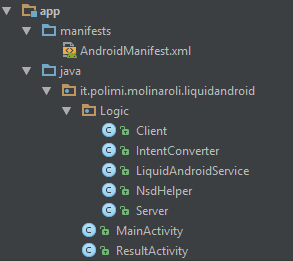
\includegraphics[width=.45\textwidth]{package}
	\caption{Code organization}
	\label{fig:5.1}
\end{figure}
As anticipated, the code is organized following the \textit{MVC} design pattern, so the \textit{controller components} are all contained in the \textit{Logic} package, while the \textit{UI components} are left inside the \textit{Main} package of the application- Other components typical of the Android development framework are left in their standard locations, such as the XML file containing the \textit{application manifest}.

\subsubsection{Implicit Intents to listen}
\lstinputlisting[language=XML , caption=Liquid Android MainActivity Manifest example, label=code:5.1]{Codici/manifest.xml}
In \lstlistingname~\ref{code:5.1} there is part of the manifest, of my application, showing some common intent filters which the \textit{Liquid Android} app can listen to. In figure we can see that is the MainActivity of the application which declare itself capable of managing intents to take a picture, send and email or open a map. By adding any intent filter to the manifest of the application Liquid Android can listen and forward, automatically any kind of Android implicit intent. This snippet of code is the way in which the \text{FR1} is practically implemented.\\\\
In the following section I want to describe my system in action, providing application's screenshots, UML diagrams, working tests and use cases.
\section{Working Demo}
This section is intended to show the reader the \textit{Liquid Android Application} while it is working. After the structure and the implementation of the application were explained it is necessary to show the finished work. As anticipated, my application
is simply a proof of concept of how it is possible to use a group of Android devices, as they were executing a single distributed operating system using well known  Android mechanisms. Users should not worry about substrates, they can control everything with a single and simple standard Android UI.\\
I set up the demo by creating a LAN with a wireless router, and then I installed my application on three smartphones, connected both to Android Studio to debug the applications reading the consoles, and to the wireless LAN. This is only one possible environment configuration for my middleware application, but is enough simple and significant to provide a proof of my work.\\
I developed, also, for testing purposes, a simple client application able to generate standard Android implicit intents, which I will use to perform some live test cases. I called this Android app, \textit{Intent Generator} which has the only feature of create intents and then ask the OS to resolve them. The same result can be obtained using any standard Android app which generates implicit intents and passes them to the OS to be solved.
\subsection{Liquid Android UI}
\begin{figure}[h]
	\centering
	\begin{minipage}{.49\textwidth}\centering
	\subfloat[Main Activity UI\label{subfig-1:main}]{%
		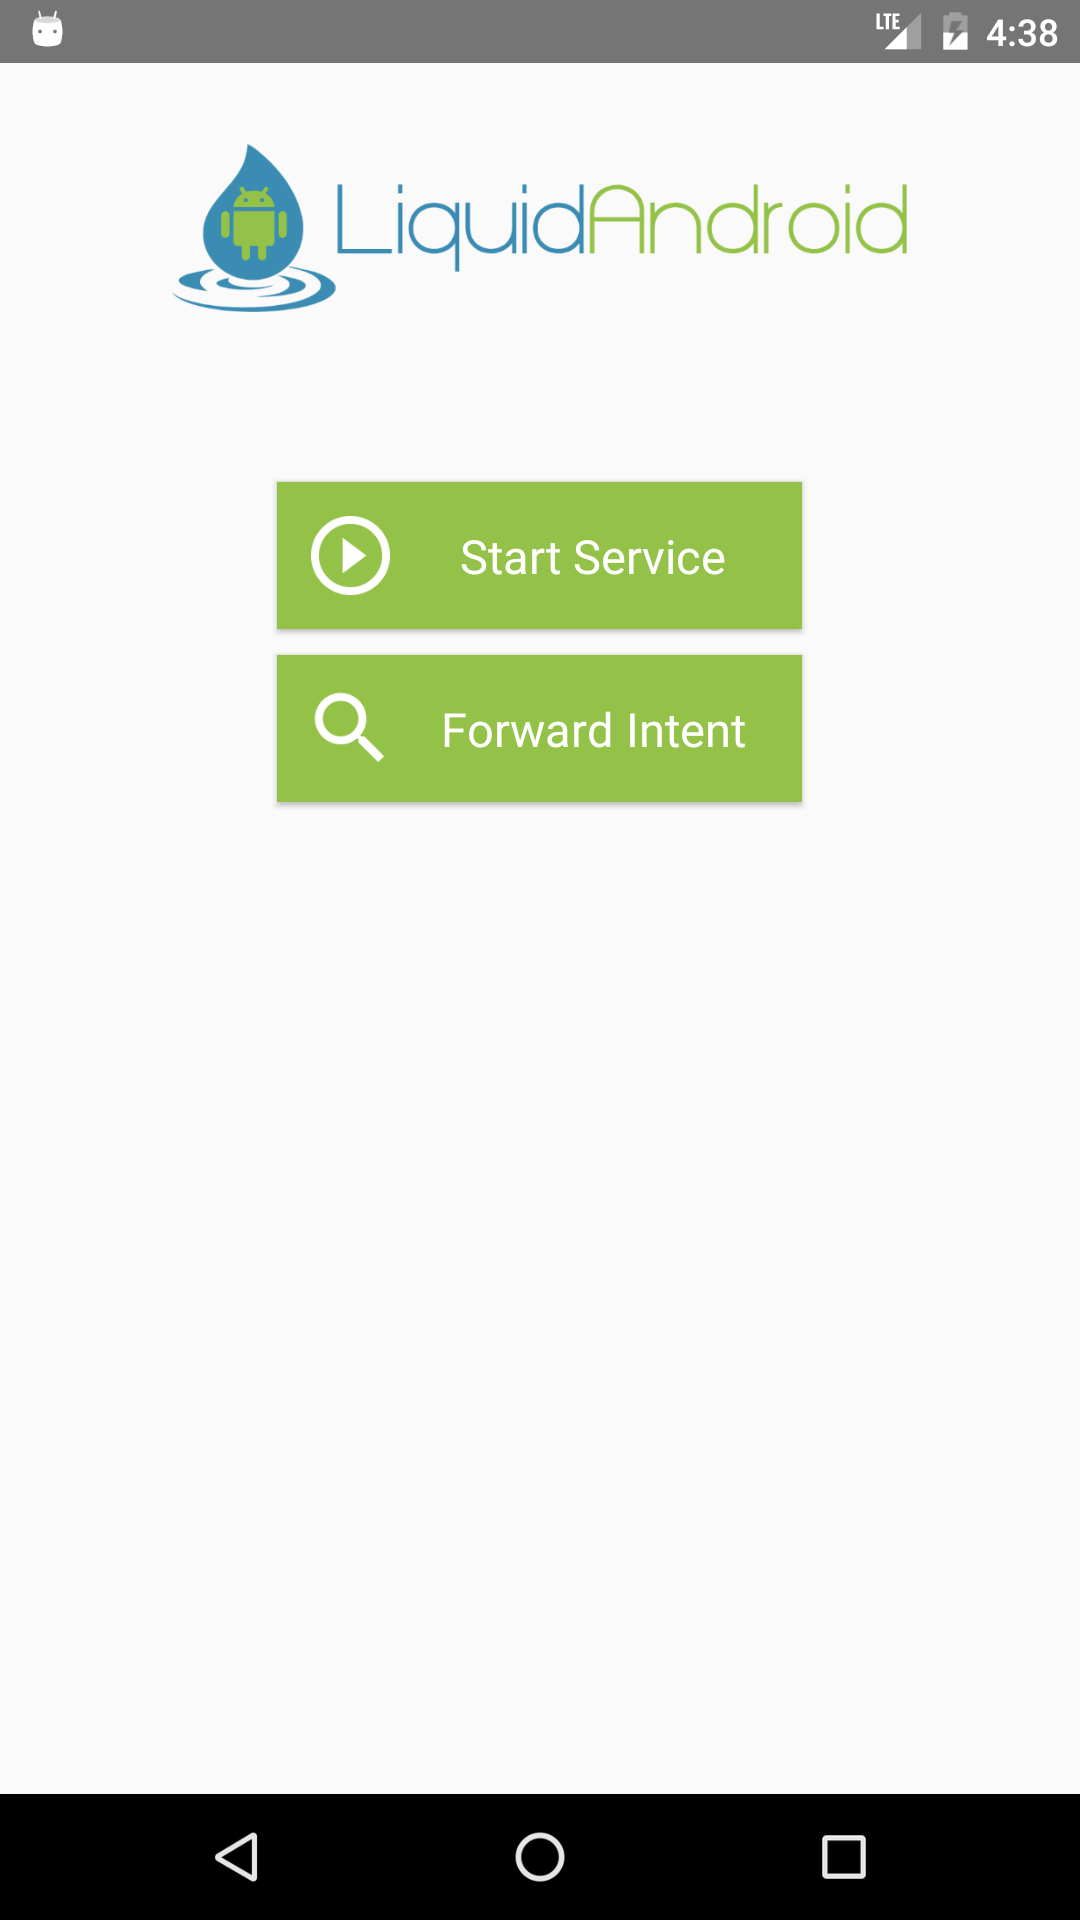
\includegraphics[width=0.75\textwidth]{main}
	}
	\end{minipage}
	\begin{minipage}{.49\textwidth}\centering
	\subfloat[Notification UI\label{subfig-2:notification}]{%
		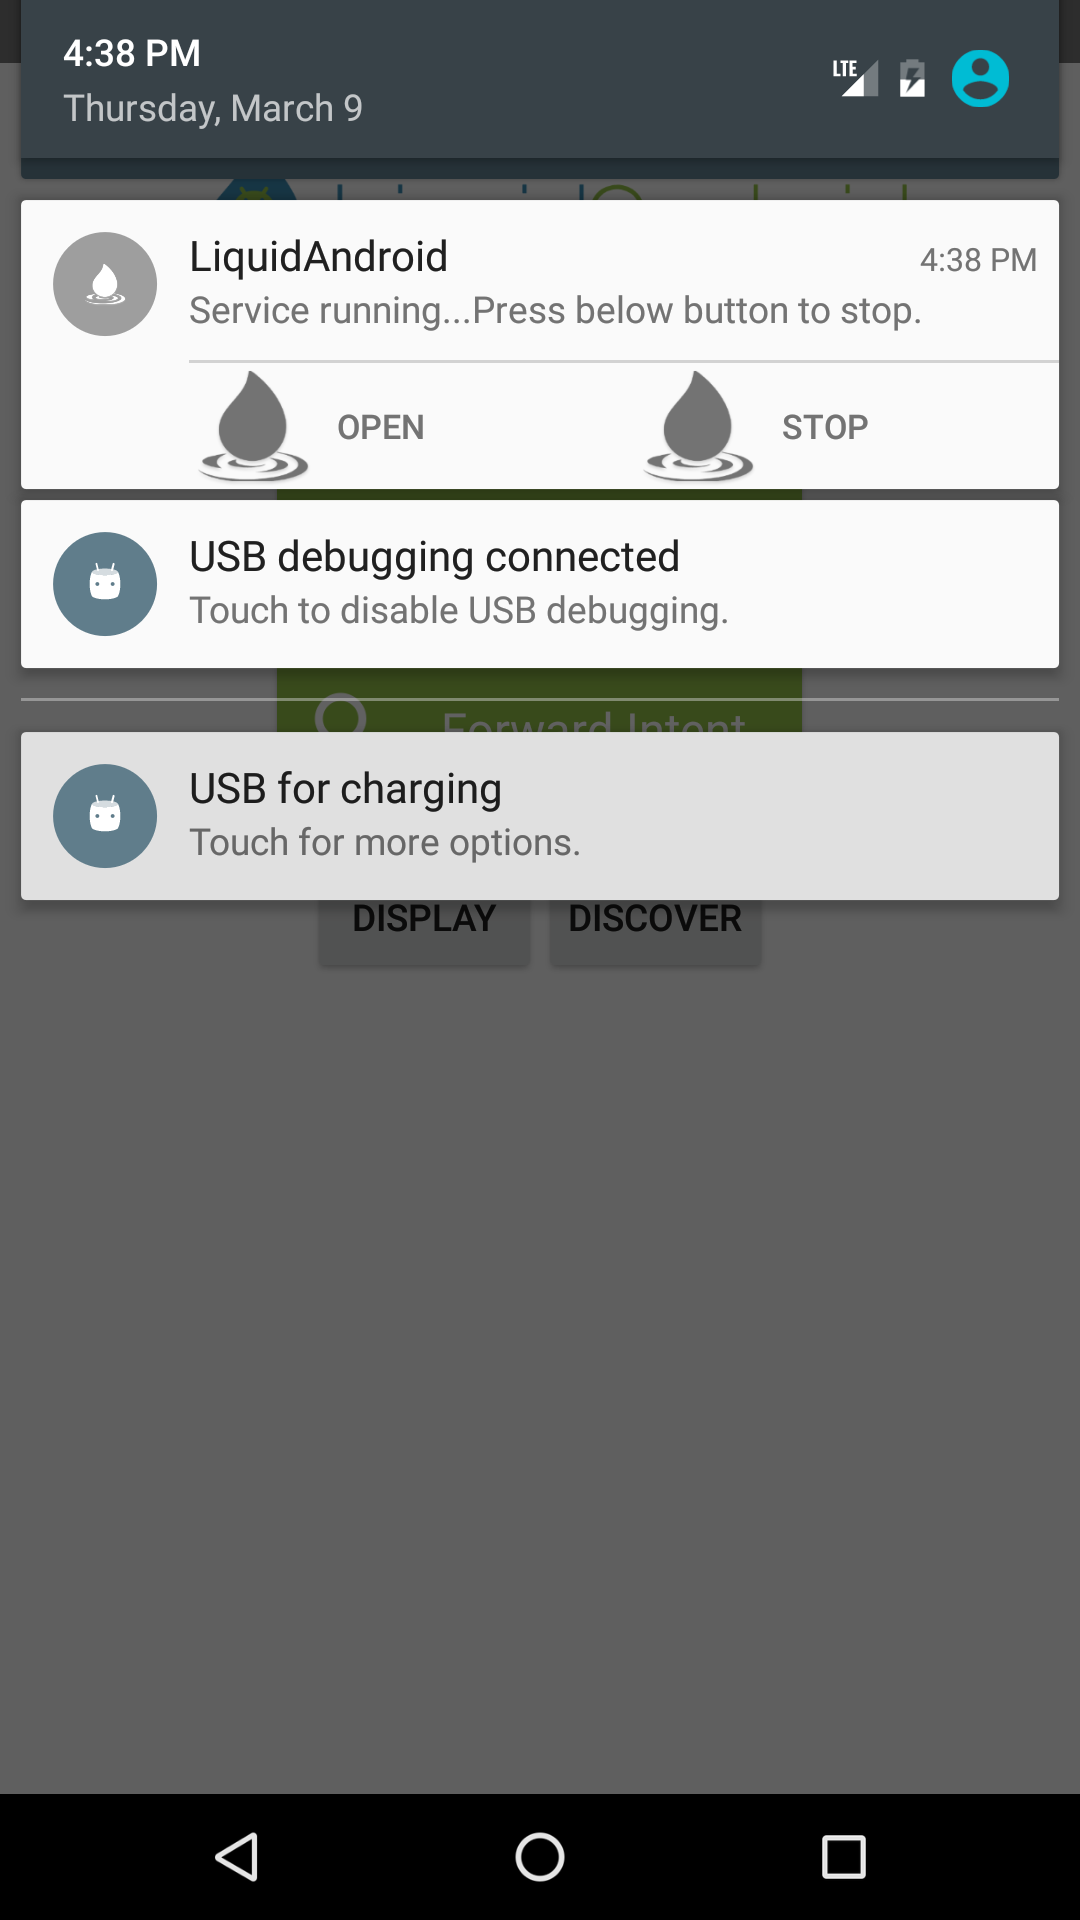
\includegraphics[width=0.75\textwidth]{notification}
	}
	\end{minipage}
	\caption{Main Liquid Android UI components}
	\label{fig:5.2}
\end{figure}

Once installed the Liquid Android application on a compatible device, users can control it by its MainActivity and its \textit{foreground service} notification, when the service is in execution. The \figurename~\ref{fig:5.2} shows the Liquid Android application's main UI components. By clicking the button \textit{Start Service} the middleware executes and the extension of the Android OS is performed by the application. Once clicked the button the server component of the application is up, and the network service is registered in the LAN, moreover the notification showed in \ref{subfig-2:notification} appears in the Android notification area. From that notification, users can control the status of the service, because it can not be removed from the Android notification area until the service is stopped by clicking the stop button, embedded in the notification. The other embedded open button, instead, starts the MainActivity, in \ref{subfig-1:main}, and puts it in foreground.\\
\begin{figure}[h]
	\centering
	\begin{minipage}{.49\textwidth}\centering
		\subfloat[App Chooser Dialog UI\label{subfig-1:intent}]{%
			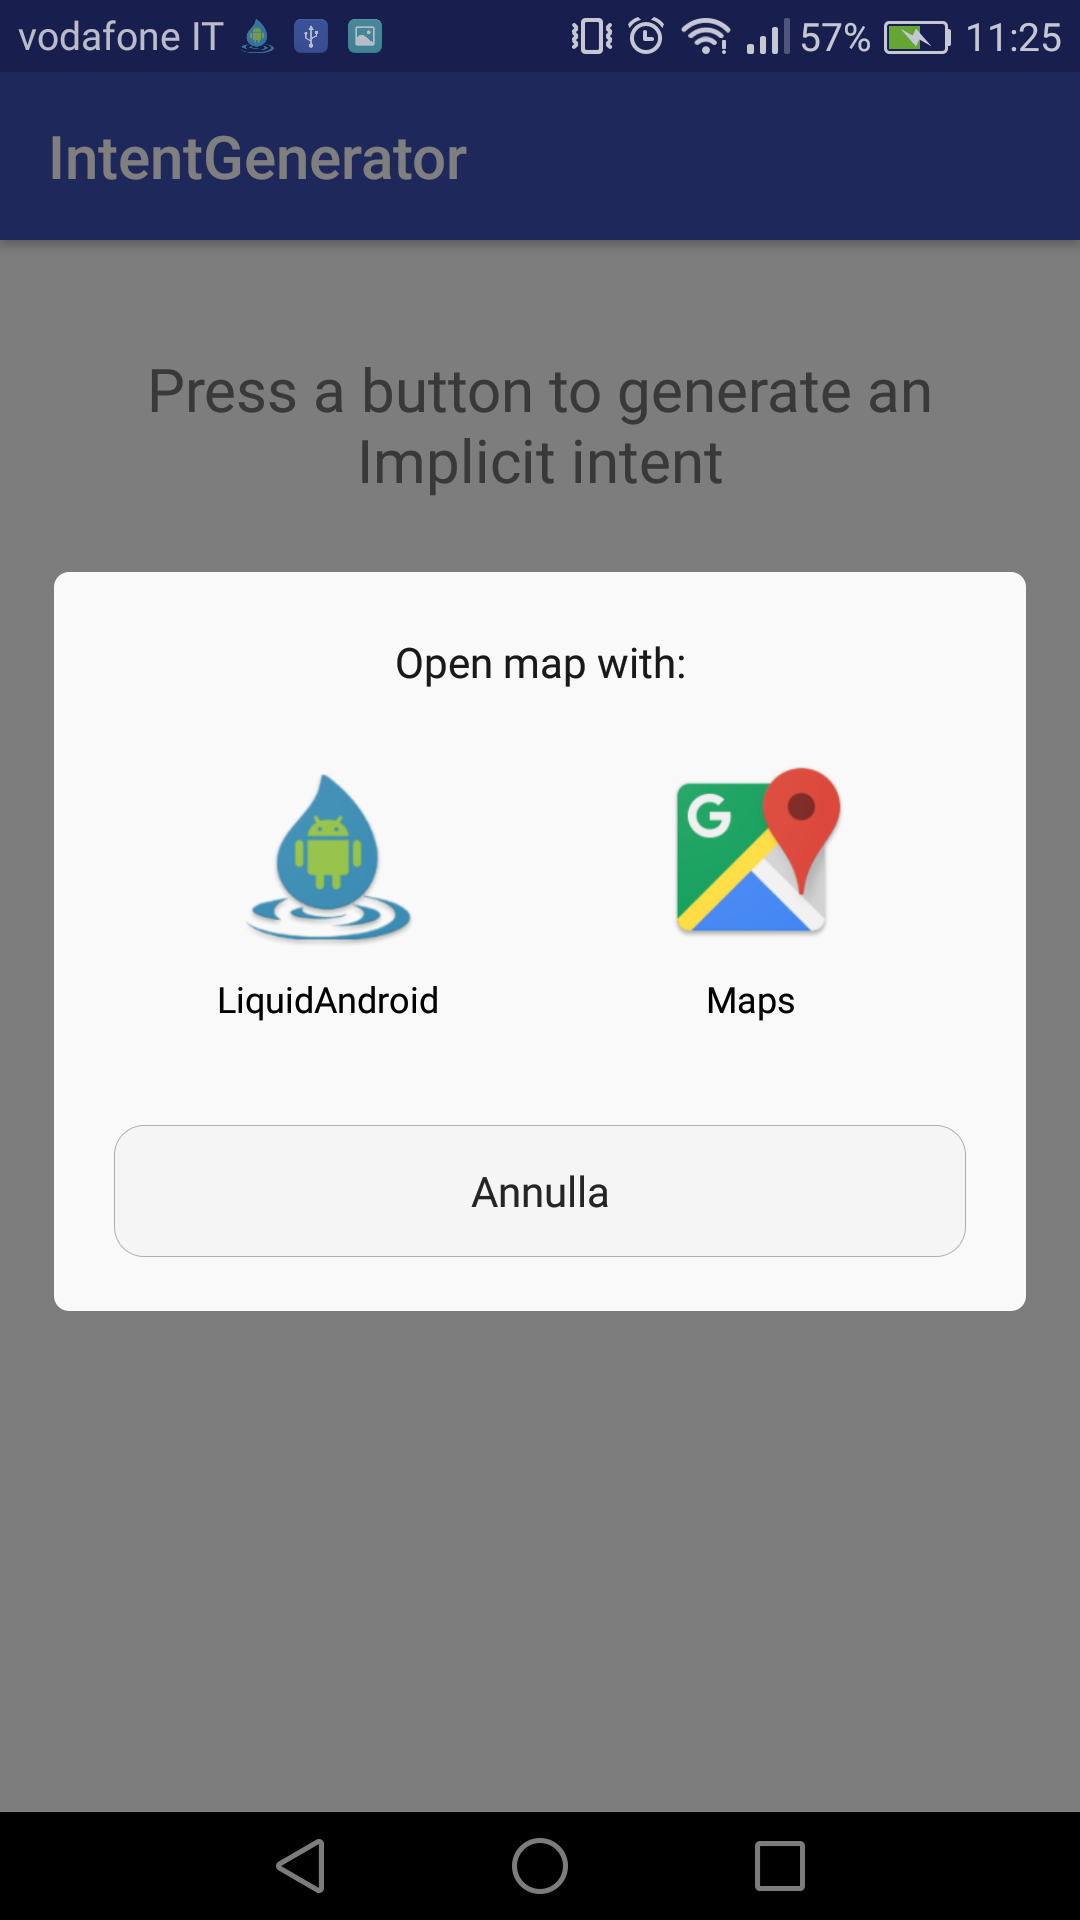
\includegraphics[width=0.75\textwidth]{selector}
		}
	\end{minipage}
	\begin{minipage}{.49\textwidth}\centering
		\subfloat[Forward Dialog UI\label{subfig-2:forward}]{%
			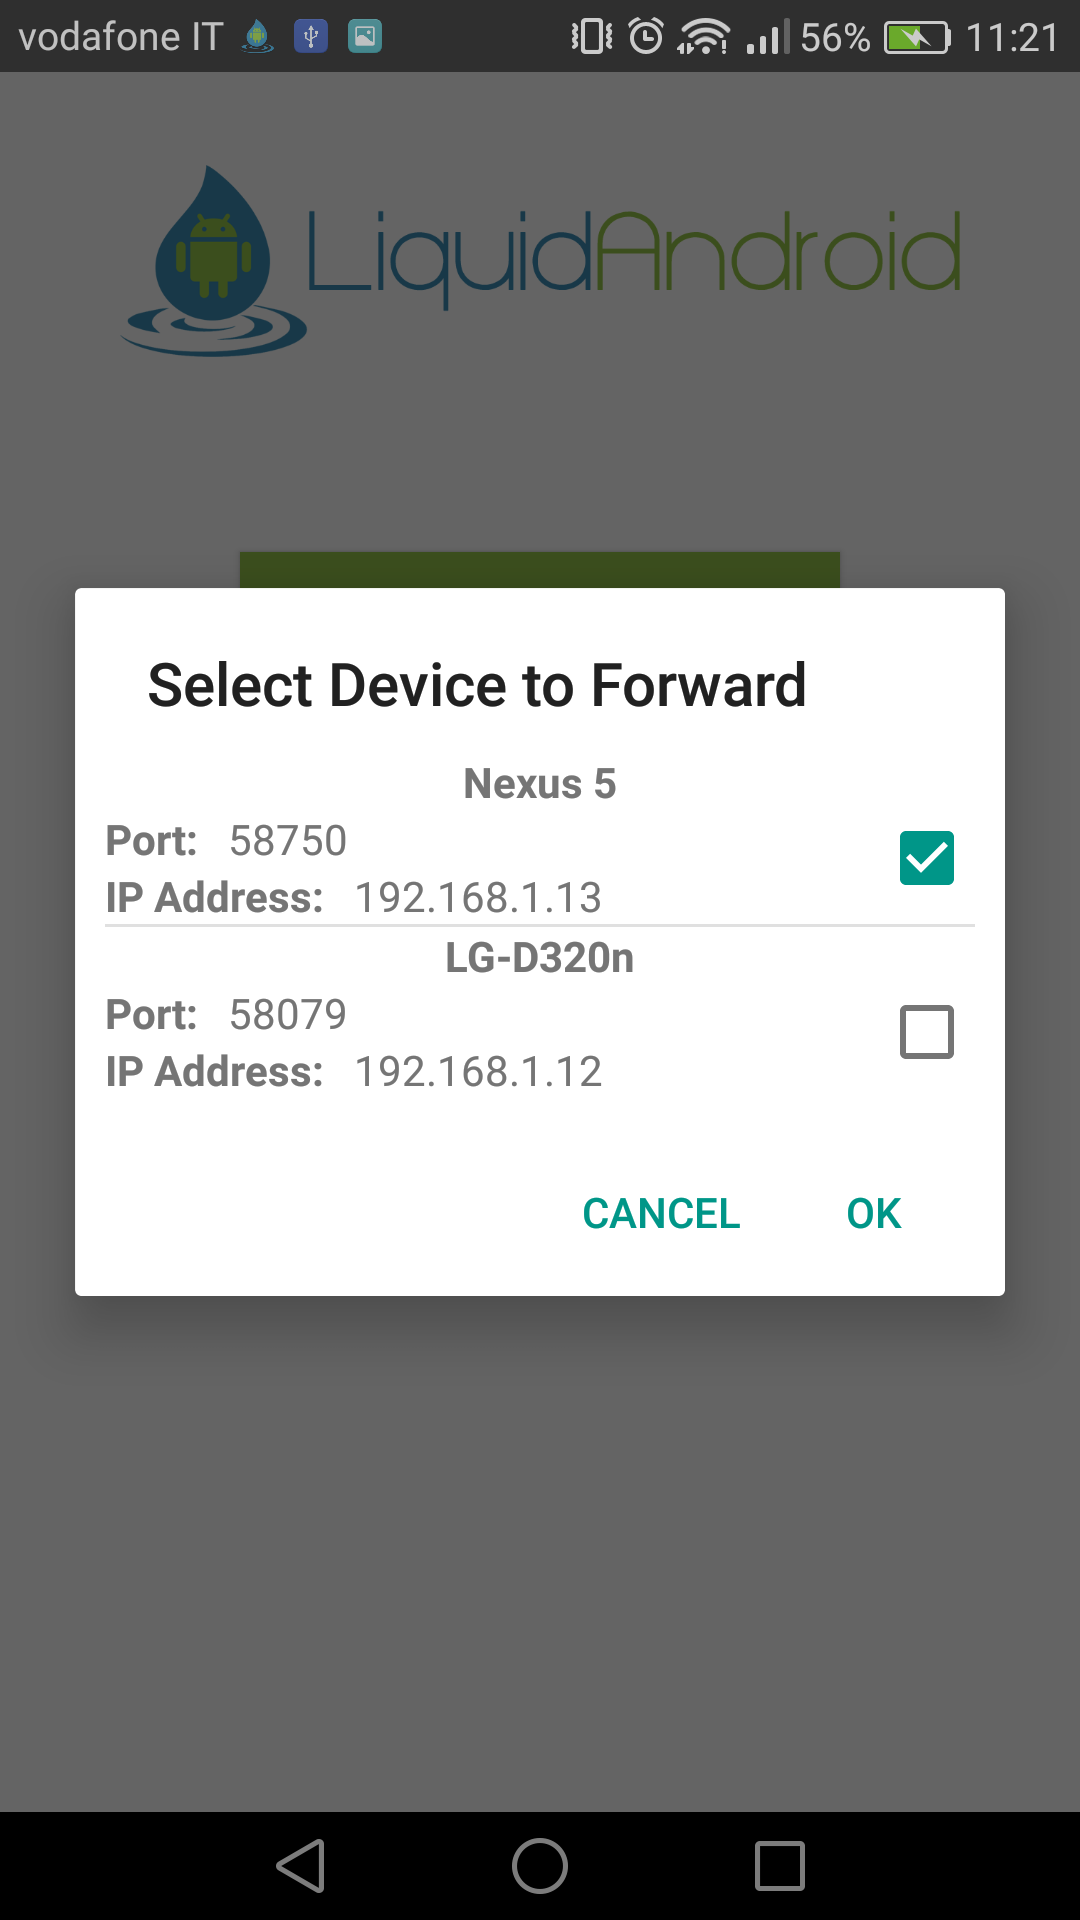
\includegraphics[width=0.75\textwidth]{alert}
		}
	\end{minipage}
	\caption{Dialogs Components}
	\label{fig:5.3}
\end{figure}
When any Android component asked the system to resolve an implicit intent, which my application can handle, the Android OS opens the \textit{App Chooser Dialog} and waits for a user choice. By selecting the Liquid Android application in the \textit{dialog} showed in \ref{subfig-1:intent}, the user ends on the MainActivity UI. Now, if the service is already in execution it can perform the forward action. The second button in the MainActivity, indeed, \textit{Forward Intent}, can be used only while the service is running. When properly clicked, it opens the \textit{Forward Dialog UI}, in \ref{subfig-2:forward}, which my middleware automatically searches for devices in the LAN with the service installed and in execution, and let the user to select on which of them forward the previously intercepted implicit intent, by ticking the \textit{check-box} as showed in the \figurename~\ref{fig:5.3}. Once selected on which device,or devices, the intent should be forwarded, by pressing the ok button, the application converts it in a JSON-Intent and sends it through the socket to them, generating Clients components which connects to the target Servers components. At this point when the message is received by the target devices, the JSON-Intent is automatically reconverted in the original Android intent, and a new intent resolution process is triggered by my application. Thus, the Android OS shows again, to the user, an \textit{App Chooser Dialog}, and lets him select with which application, among the listed ones, perform the intent task.
\begin{figure}[h]
	\centering
	\begin{minipage}{.49\textwidth}\centering
		\subfloat[App Chooser\label{subfig-1:appchooser}]{%
			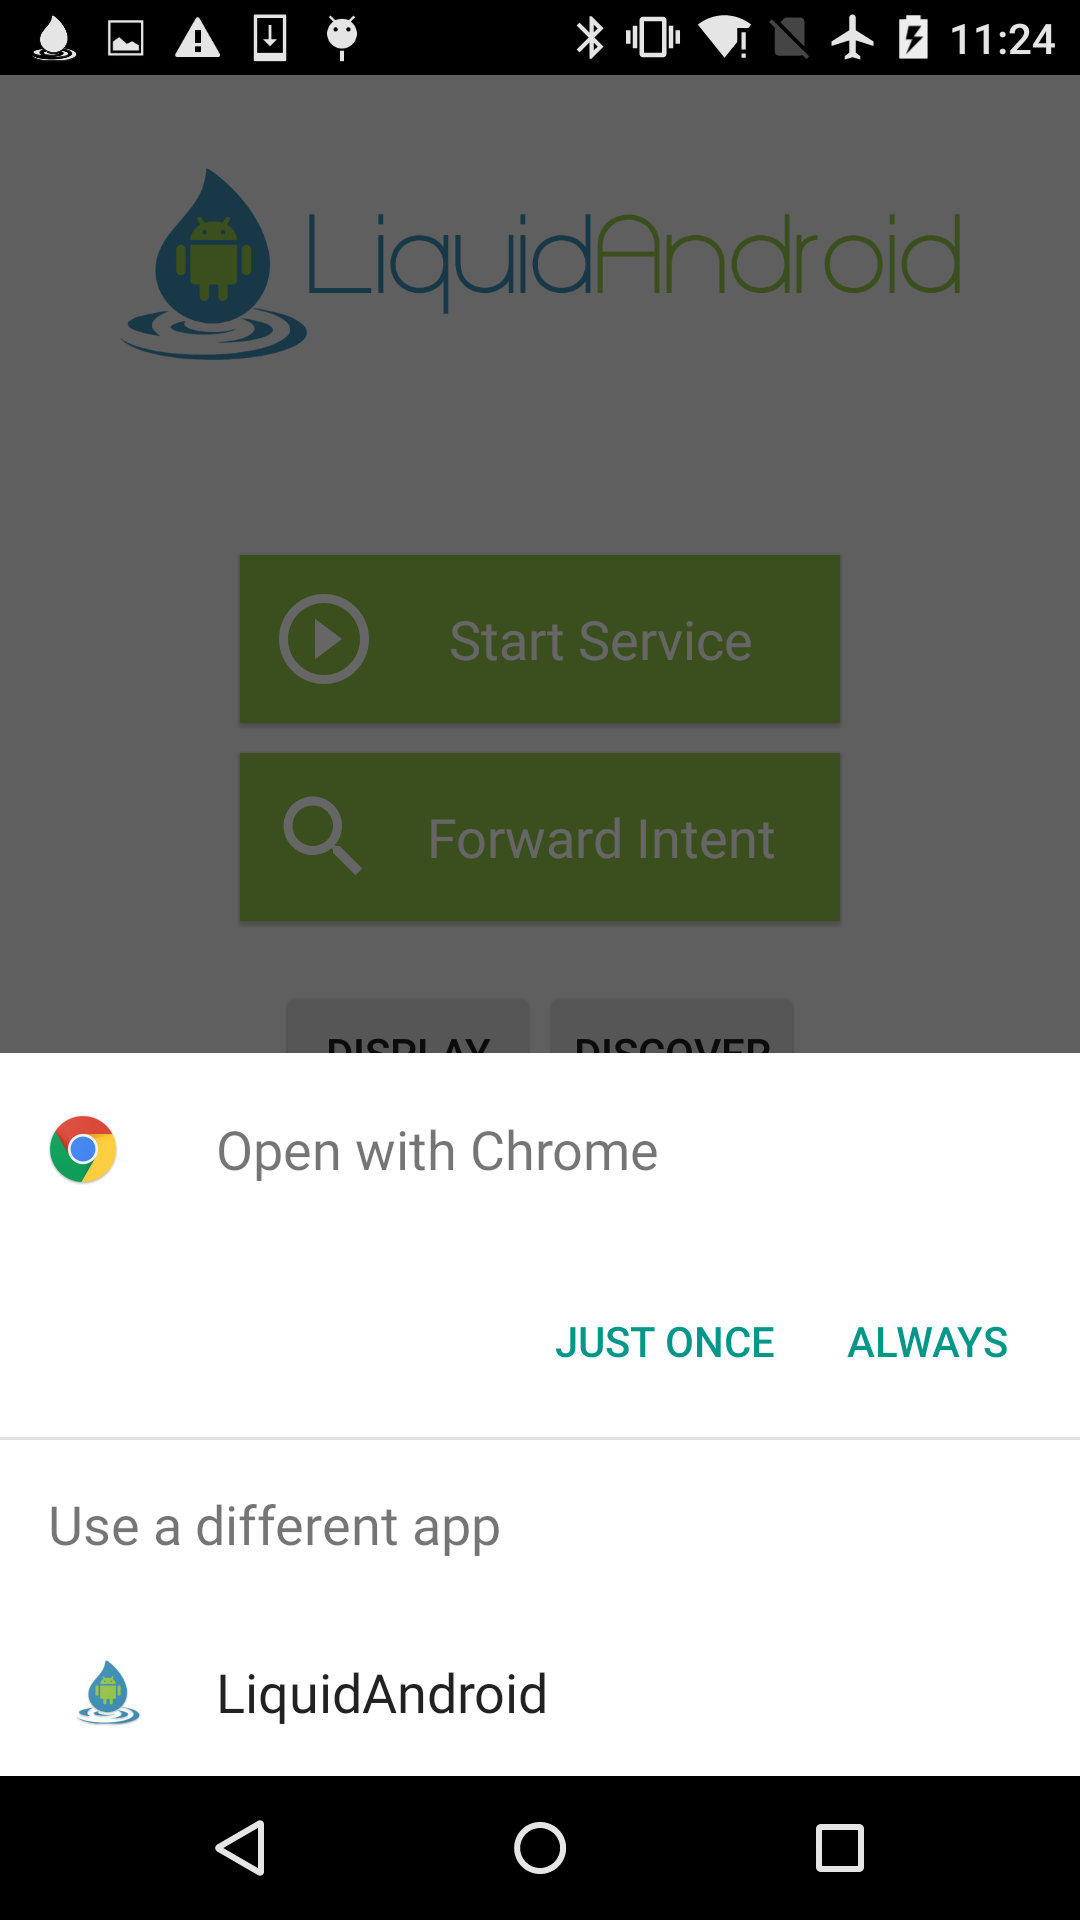
\includegraphics[width=0.75\textwidth]{appchoser}
		}
	\end{minipage}
	\begin{minipage}{.49\textwidth}\centering
		\subfloat[Third party Browser Activity\label{subfig-2:browser}]{%
			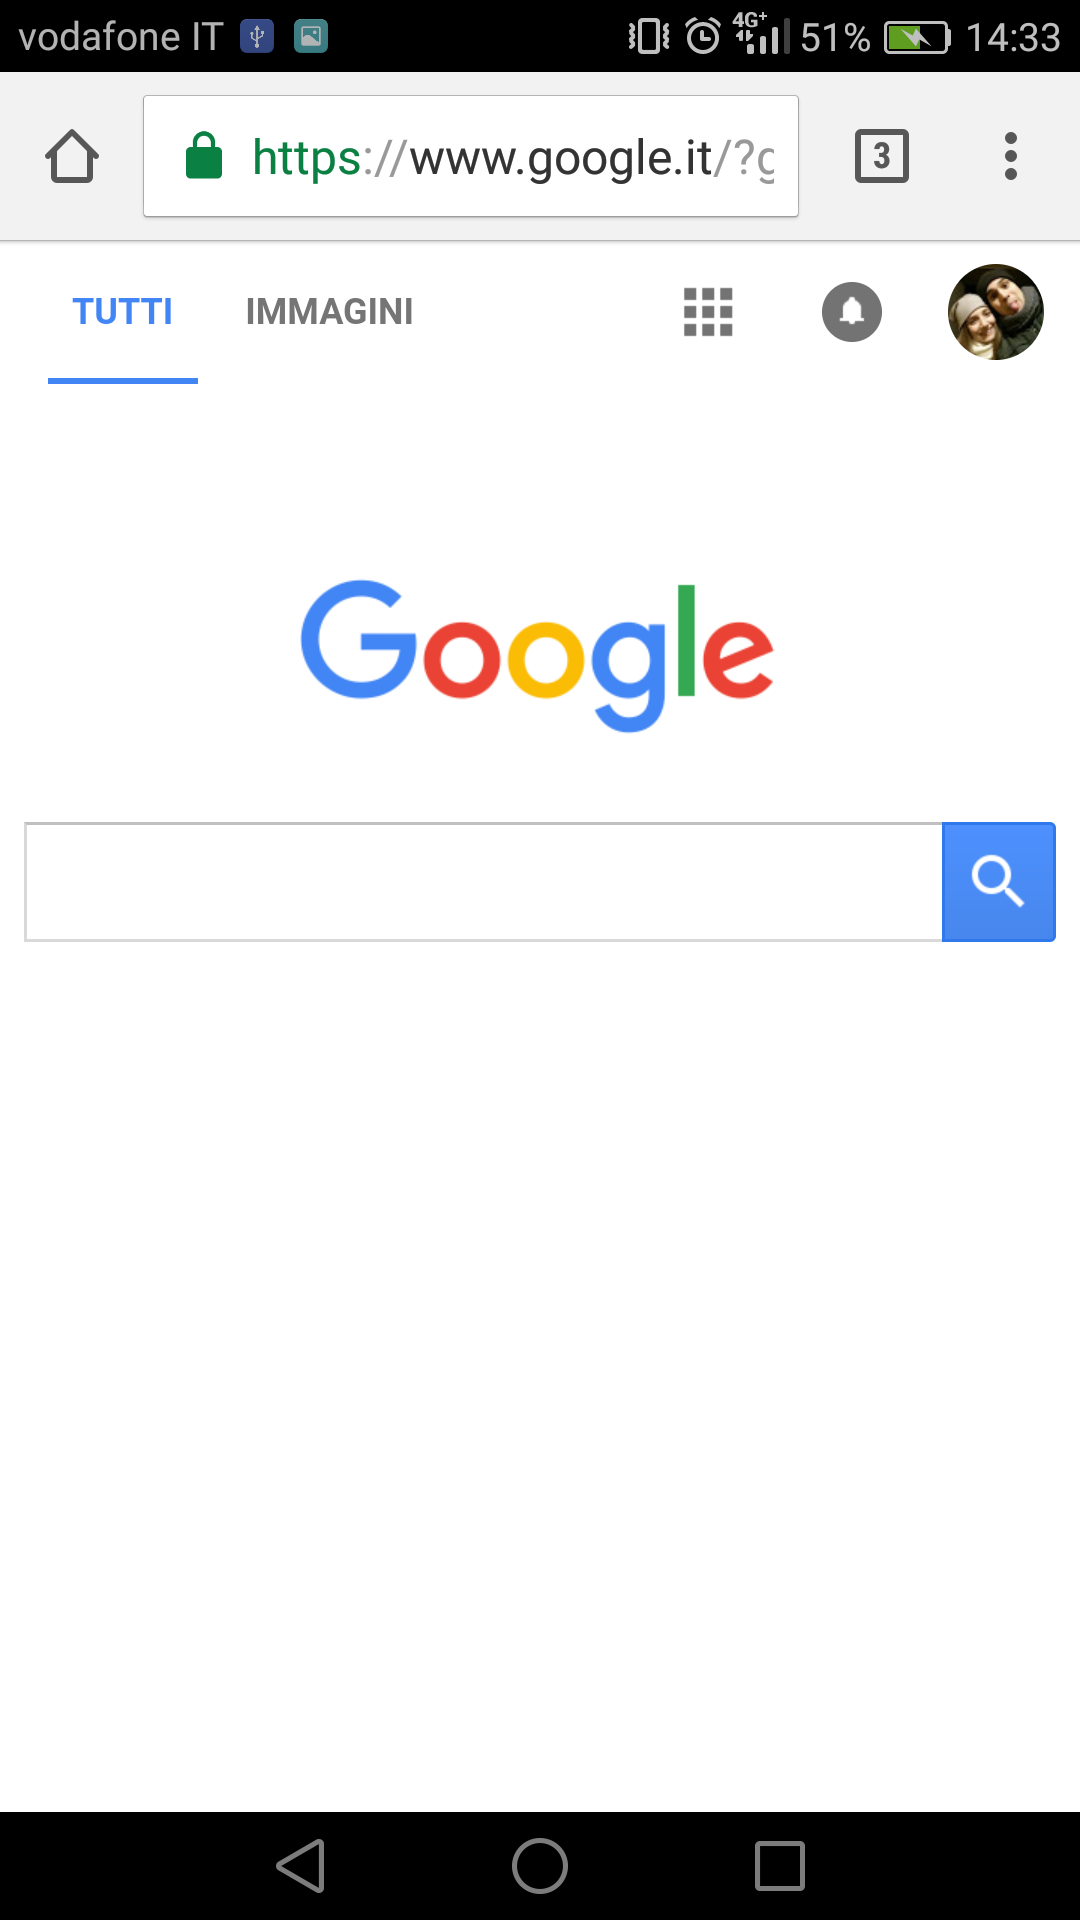
\includegraphics[width=0.75\textwidth]{browser}
		}
	\end{minipage}
	\caption{JSON-Intent execution}
	\label{fig:5.4}
\end{figure}
The \figurename~\ref{fig:5.4} describes the working mechanism above explained, in this particular case the devices received an intent to view the web-page \textit{http://Google.it}. By selecting, in \ref{subfig-1:appchooser}, \textit{Open with Chrome}, the process terminates with the execution of the browser activity, in \ref{subfig-2:browser}, showing exactly that page.

\subsection{Live Test Cases}
In this subsection I want to present two live tests I performed to prove that my application respects all the constrains and fulfill all the functional, and also non-functional, requirements.
As already explained, I created a second simple Android application working as a client for the Liquid Android middleware. This application \textit{Intent Generator} is composed by a single activity in which there are some buttons to let the user create easily implicit intents to be resolved by the Android OS.
\begin{figure}[h]
	\centering
	\begin{minipage}{.49\textwidth}\centering
		\subfloat[Intent Generator MainActivity\label{subfig-1:intentmain}]{%
			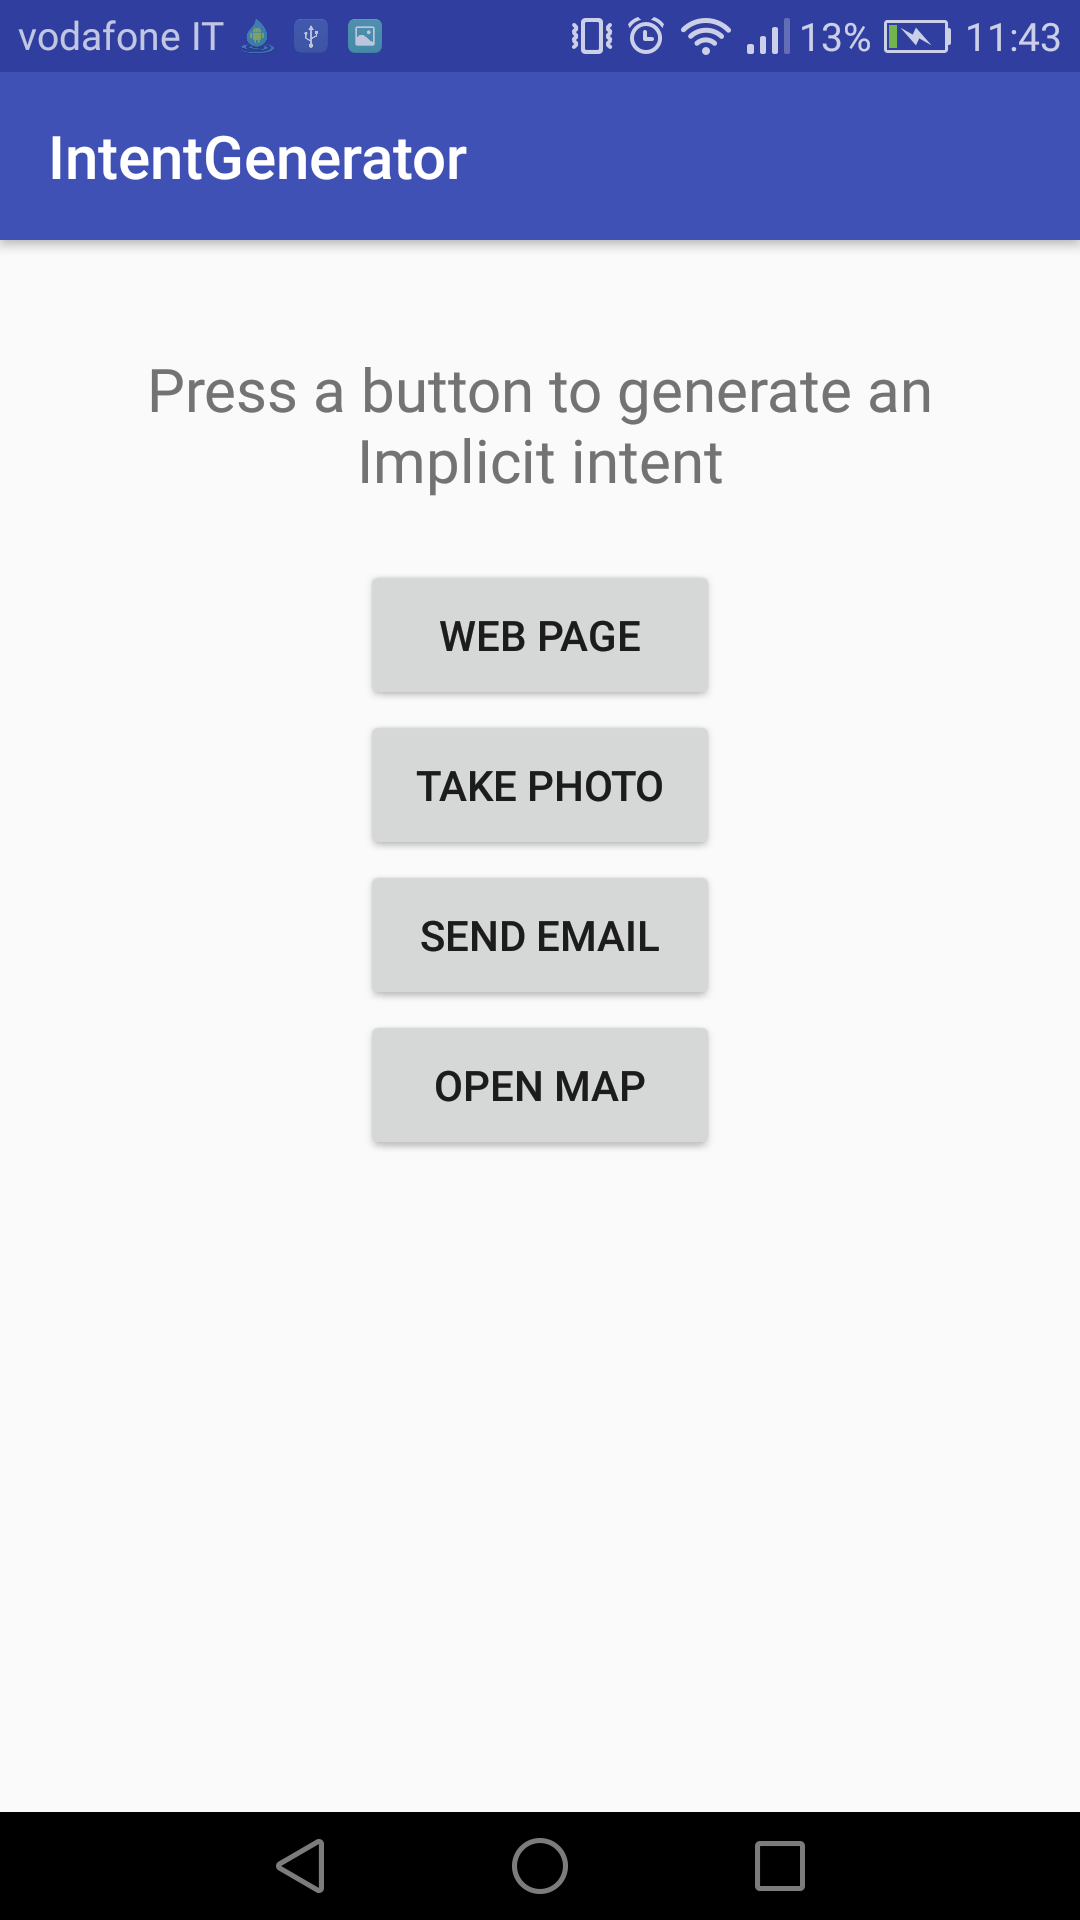
\includegraphics[width=0.75\textwidth]{intentgenerator}
		}
	\end{minipage}
	\begin{minipage}{.49\textwidth}\centering
		\subfloat[Intent Generator data Picker\label{subfig-2:picker}]{%
			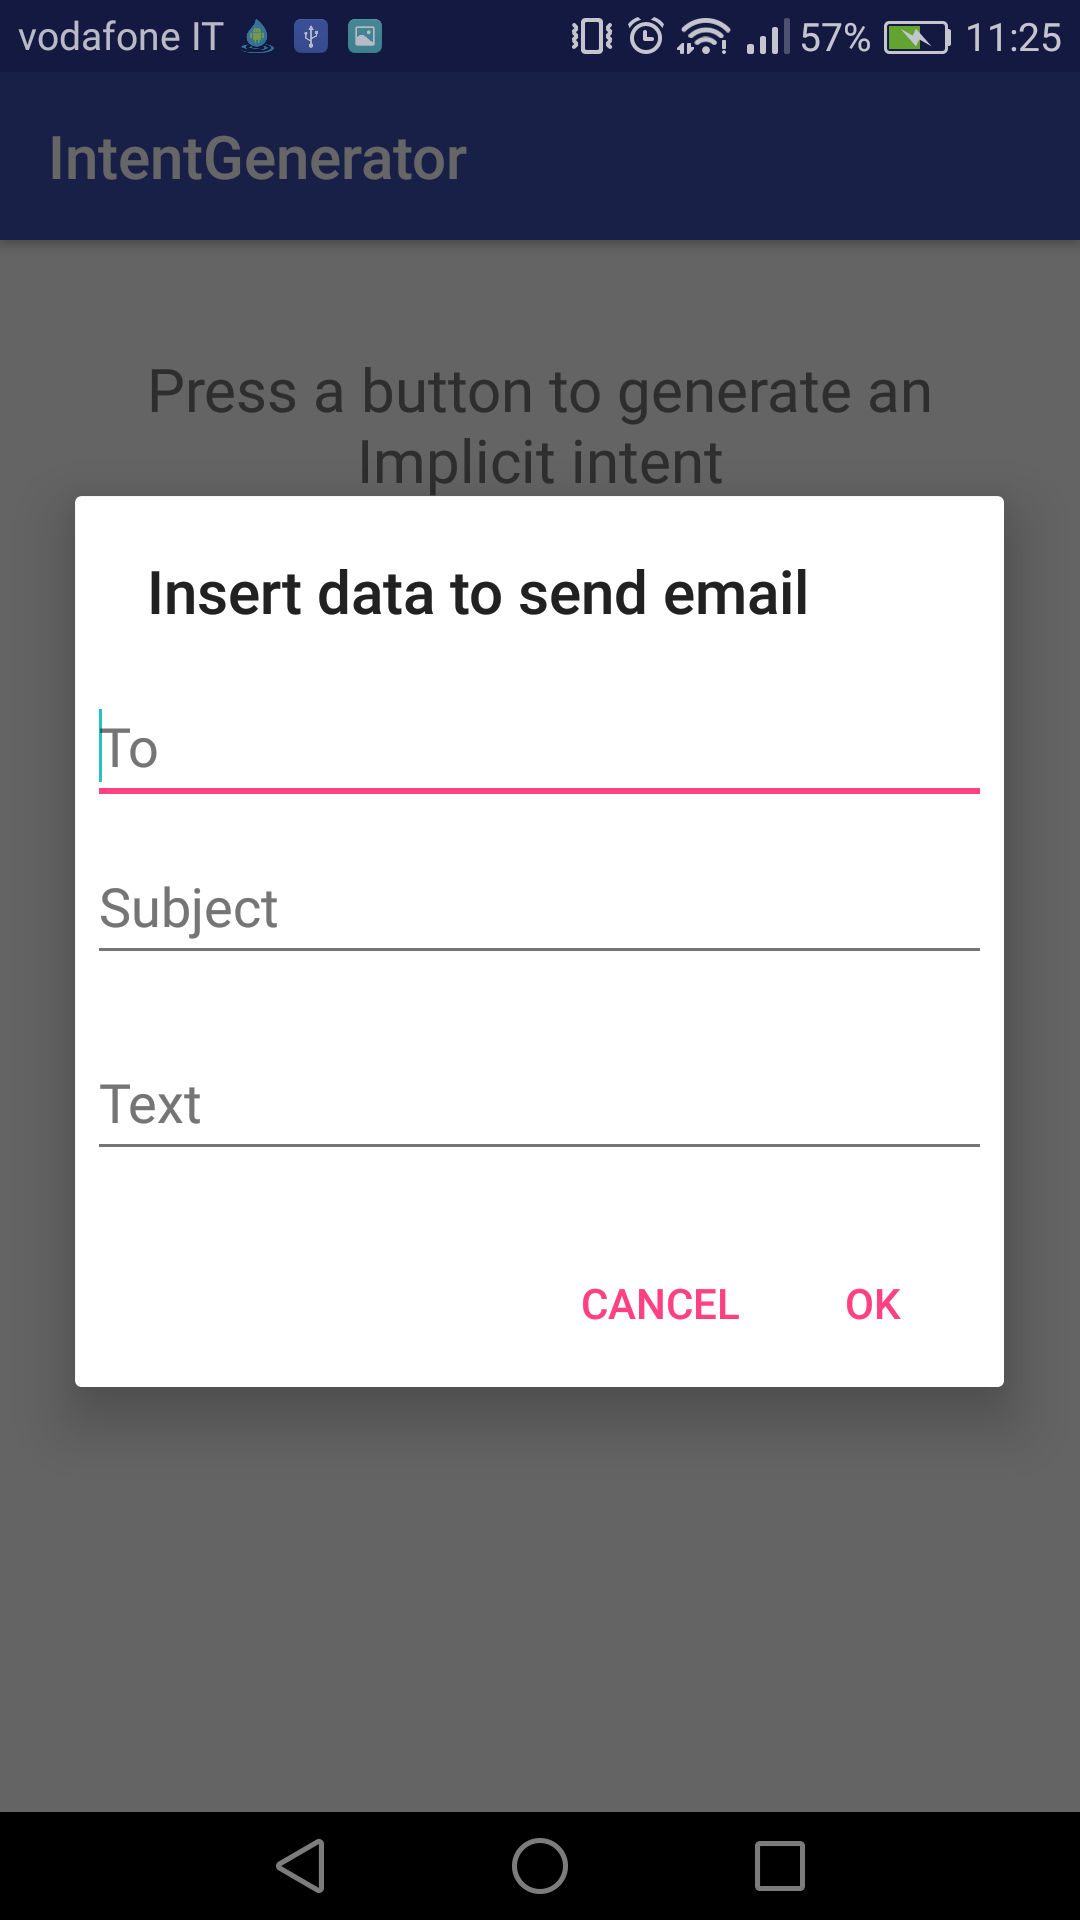
\includegraphics[width=0.75\textwidth]{picker}
		}
	\end{minipage}
	\caption{Intent Generator UI}
	\label{fig:5.5}
\end{figure}
In \figurename~\ref{fig:5.5} there are two screenshots of the \textit{Intent Generator} application. In \ref{subfig-1:intentmain}, there is the main activity, with which I generate some common implicit intents, to be forwarded using the Liquid Android middleware, by simply pressing the desired button in the UI. When the intent to be generated needs extra data the applications shows a \textit{Dialog Picker} to let insert additional data to the intent, as shown, in \ref{subfig-2:picker}, when the \textit{SEND EMAIL} button is pressed.\\
By using this environment I have performed the tests I am presenting in this section. Both test cover all the functionalities the systems must have, taking in to account, also the data management problem. The first test is use the system to forward an intent to send a text email from one device to another in the system. The second one is a bit more complicated, one device of the network ask two other devices to take a picture with their camera and then to have the taken photos back.
\subsubsection{Send Email Live Test}
In this live test scenario I assume that there are two Android devices, with the Liquid Android middleware application already installed and with the service in execution.
In \figurename~\ref{fig:5.6} it is shown the complete UML sequence diagram, which completely describes this live test.\\
The first device starts the process by using the Intent Generator MainActivity, precisely by pressing the \textit{SEND EMAIL} button, already shown in \ref{subfig-1:intentmain}. Then he compiles the fields in the dialog and, once done, the implicit intent is created by the application and passed to the Android OS. The OS looks for activities capable of handling the so generated intent, and ask the user, by showing the App Chooser, with which compatible application he wants to resolve the intent. In this case the user selects the liquid android application, and ends on its MainActivity.\\
At this point the \textit{Forward Intent button} is pressed and the intent is automatically converted and sent to the selected device/s. When the intent arrives to the target, the Liquid Android Service reconverts it in an intent object to be executed and passes it to the OS.
\begin{figure}[h]
	\centering
	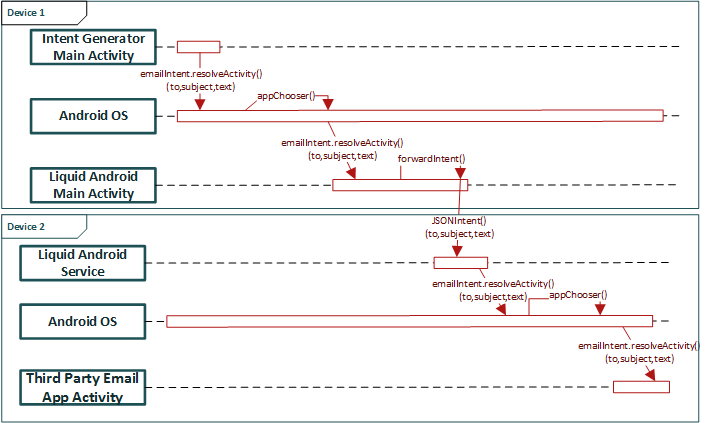
\includegraphics[width=1\textwidth]{sequence1}
	\caption{Live test 1 Sequence Diagram}
	\label{fig:5.6}
\end{figure}
The Android OS starts again a resolution process and at the end shows again the App Chooser. Now the user selects the Gmail application and completes the action by sending the email from the Gmail activity, already filled with the data the user inserted in the first device.\\
In \figurename~\ref{fig:5.7} there is the complete flow of actions presented with some real screenshots of the applications I have developed. In particular the screens from \textit{a} to \textit{d} are taken from the first device I have used, a Huawei P9, and screens \textit{e} and \textit{f} are taken from the target device, a LG L70.
\\\\
\begin{figure}[h]
	\centering
	\begin{minipage}{.24\textwidth}\centering
		\subfloat[Send Email\label{subfig-1:intentg}]{%
			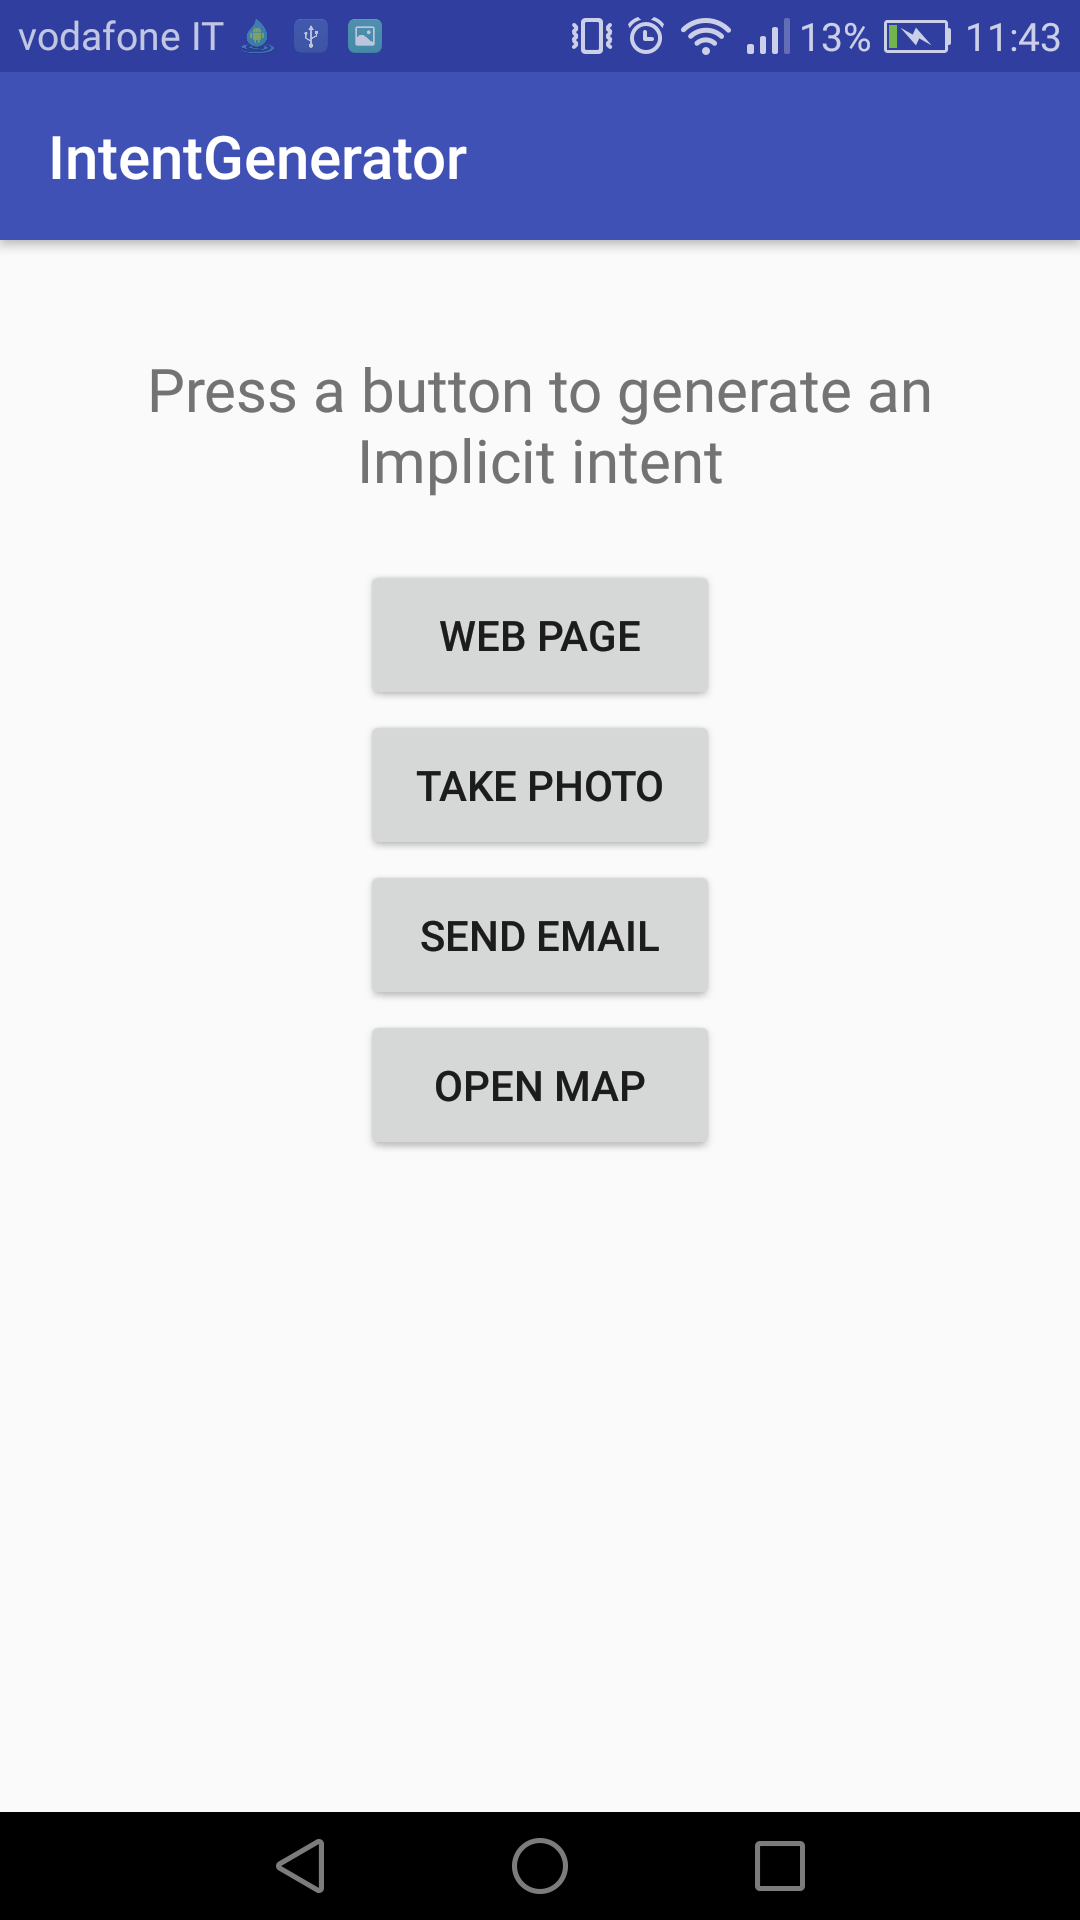
\includegraphics[width=0.9\textwidth]{intentgenerator}
		}
	\end{minipage}
	\begin{minipage}{.24\textwidth}\centering
		\subfloat[Picker Dialog\label{subfig-2:chooser}]{%
			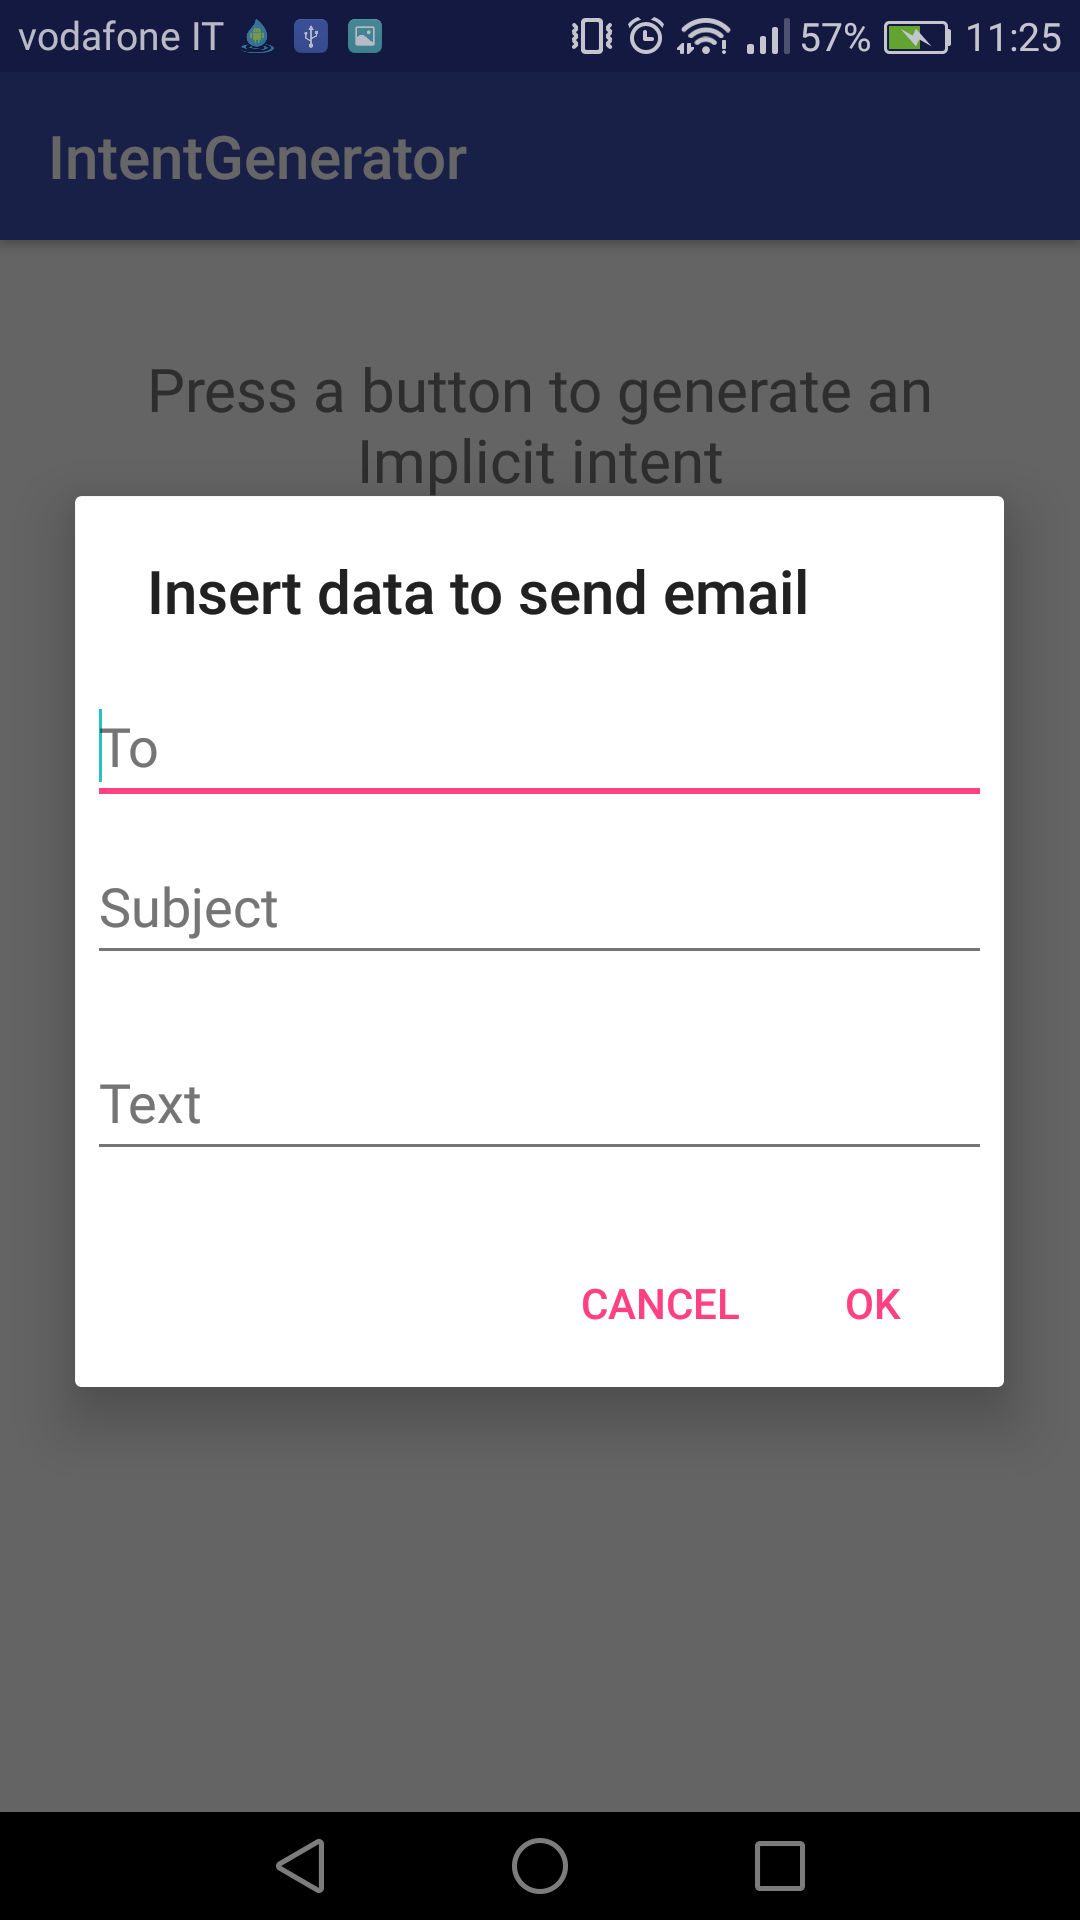
\includegraphics[width=0.9\textwidth]{picker}
		}
	\end{minipage}
	\centering
	\begin{minipage}{.24\textwidth}\centering
		\subfloat[App Chooser\label{subfig-3:liquid}]{%
			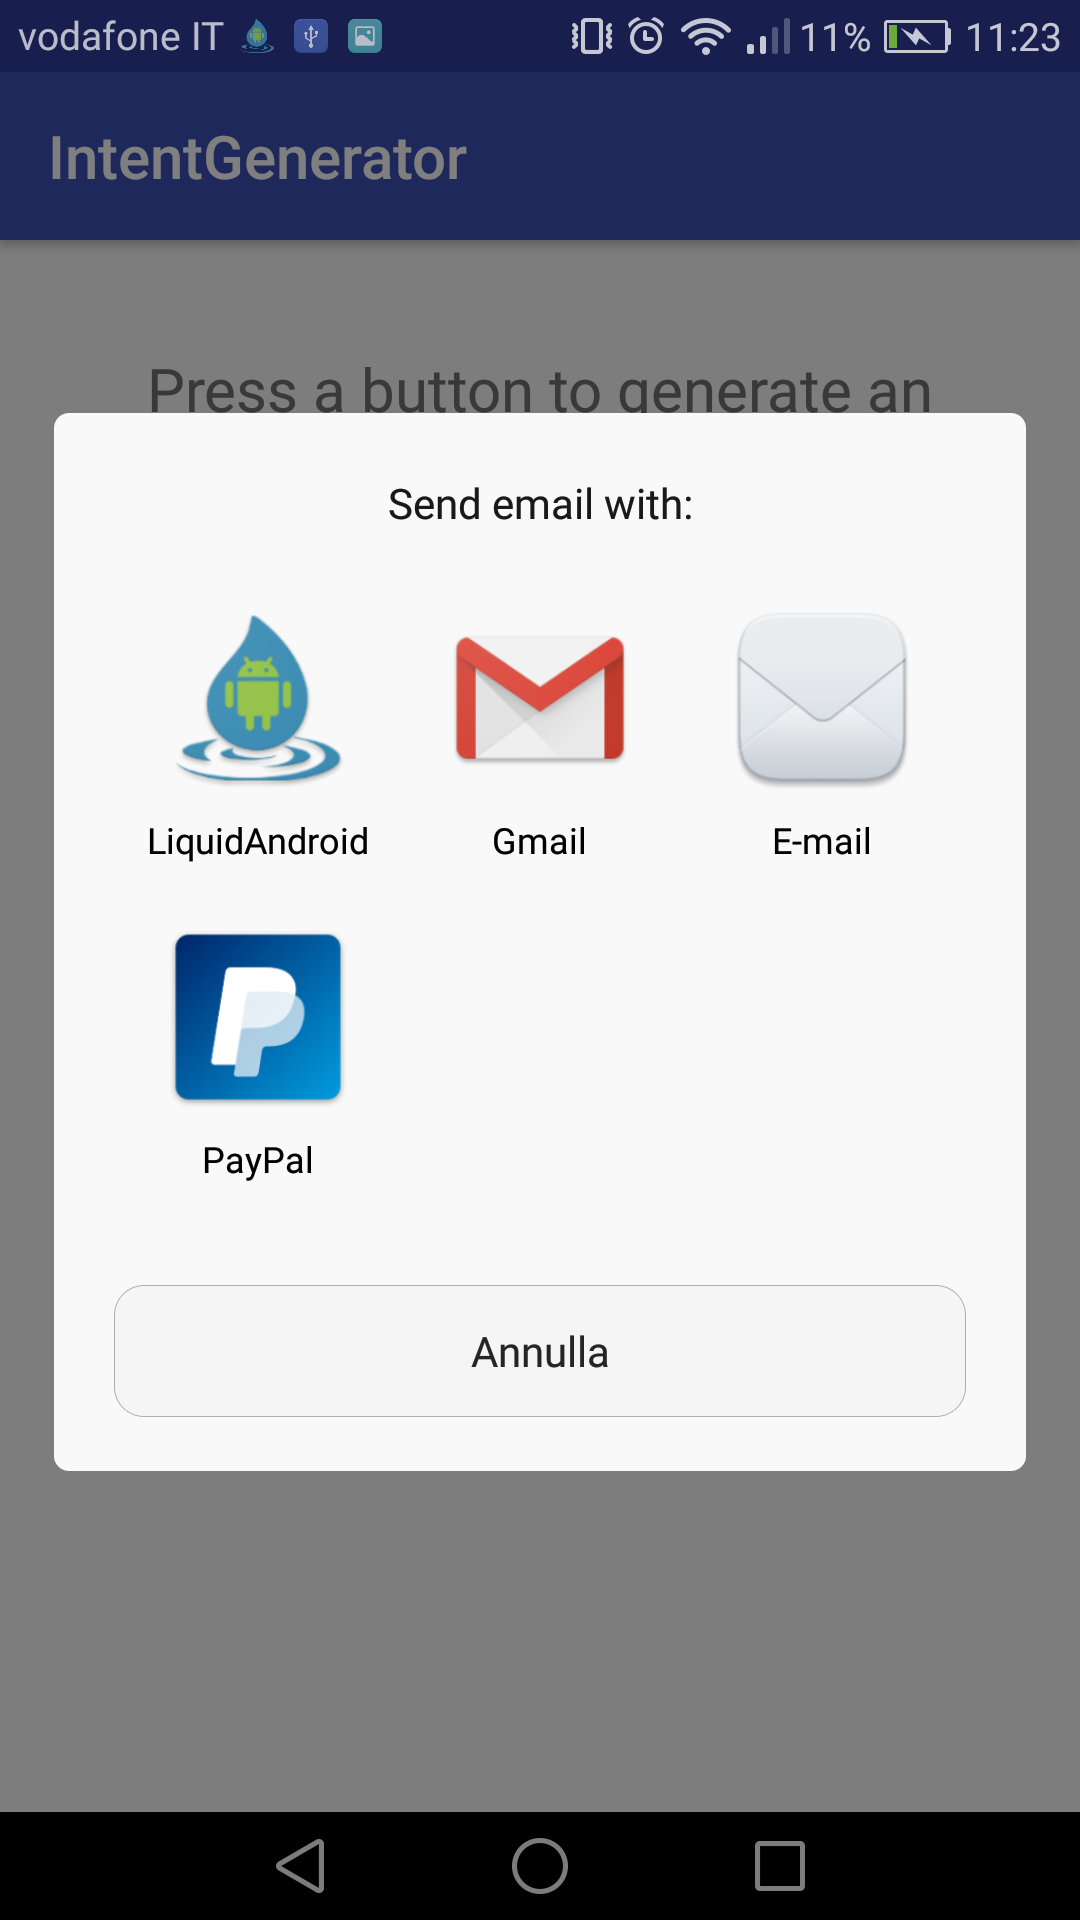
\includegraphics[width=0.9\textwidth]{sendwith}
		}
	\end{minipage}
	\begin{minipage}{.24\textwidth}\centering
		\subfloat[Forward Dialog\label{subfig-4:chooser2}]{%
			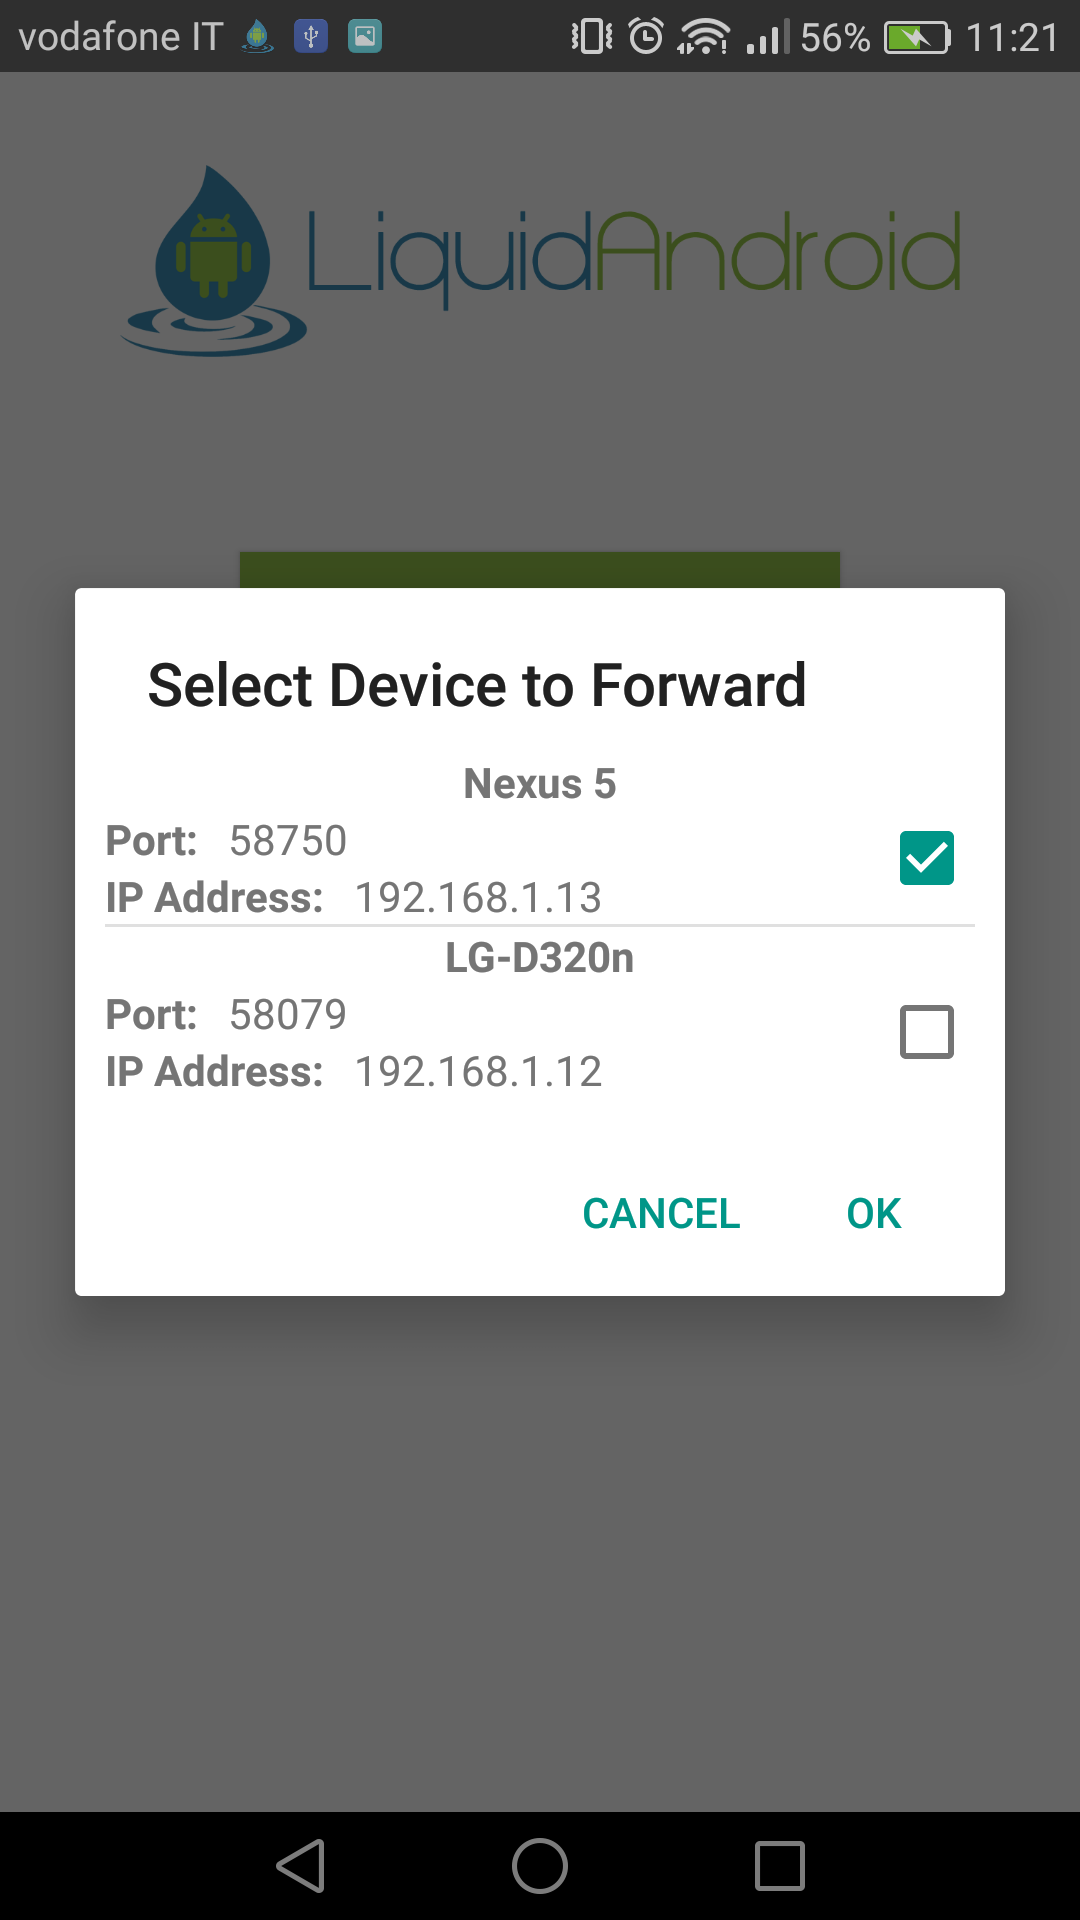
\includegraphics[width=0.9\textwidth]{alert}
		}
	\end{minipage}
	\phantomcaption 
	\label{fig:5.7}
\end{figure}

\begin{figure}[h]
\ContinuedFloat
\centering
\begin{minipage}{.24\textwidth}\centering
	\bigskip
	\subfloat[App Chooser\label{subfig-5:chooser2}]{%
		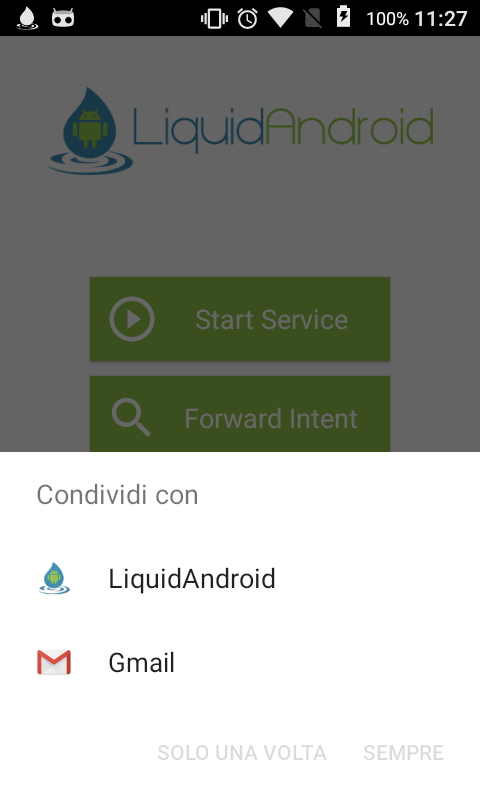
\includegraphics[width=0.9\textwidth]{condividicon}
	}
\end{minipage}
\begin{minipage}{.24\textwidth}\centering
	\bigskip
	\subfloat[Gmail Activity\label{subfig-6:chooser}]{%
		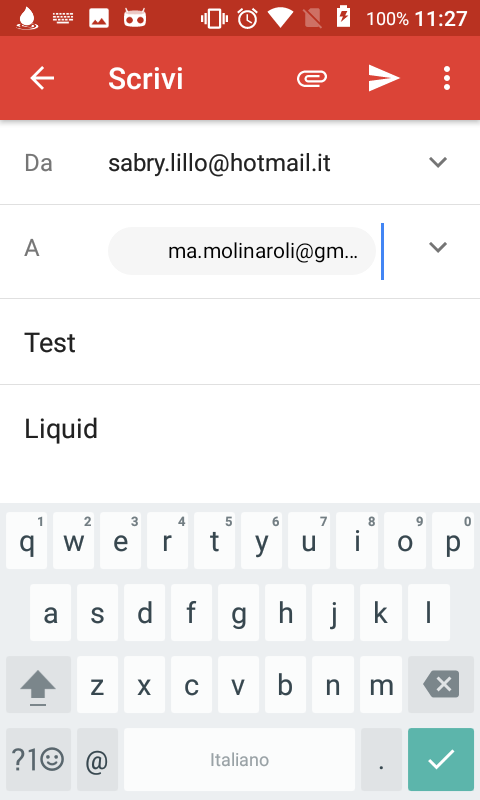
\includegraphics[width=0.9\textwidth]{gmail}
	}
\end{minipage}
\caption{Complete email live test screenshots}
\end{figure}
\subsubsection{Take Photo Live Test}
The second test I want to report exploits the Android \textit{startActivityforResult()} mechanism: it handles more complex data, and returns them to the caller. The environment I have used is exactly the one described in the previous test: three Android devices connected in the same LAN with the Liquid Android application already installed, and the background service already in execution. I want to prove that the middleware can work with more than two devices and how it manages concurrent requests. To do this I want that one device in the network, ask the other two devices to pick a photo at the same time, and once done, send the two different picture, taken with two different devices, to the original caller. I started the test by using the Intent Generator app, to generate the photo intent. When the intent is triggered the Android OS opens the app Chooser, showing the Liquid Android application as an alternative to resolve the intent. I have forwarded the intent, using the forward button, and sent it to the other two devices in the network. Once the intent arrived, the Liquid Android service triggers it, and passes it to the Liquid Android Result Activity, which starts the Android camera waiting for results. Once the user have taken the photo, with the camera, the Results Activity brings it, and send the picture back to the caller. When the picture arrives back to the caller the Liquid Android application, shows it in its Result activity. Since the intent was forwarded in two devices, when the two picture are sent back to the caller, the two result are concurrent. My system allows that concurrency by accepting different calls using different threads and then it puts in foreground the last call arrived using a LIFO policy. This complete test scenario is described, as done with the other test, showing the interaction of the components, and their activation in the UML sequence diagram in \figurename~\ref{fig:5.8}. In the diagram only two devices are present, but the third device involved in the test has exactly the same behavior the \textit{device 2} showed in the picture.\\\\\\\\
\begin{figure}[h]
	\centering
	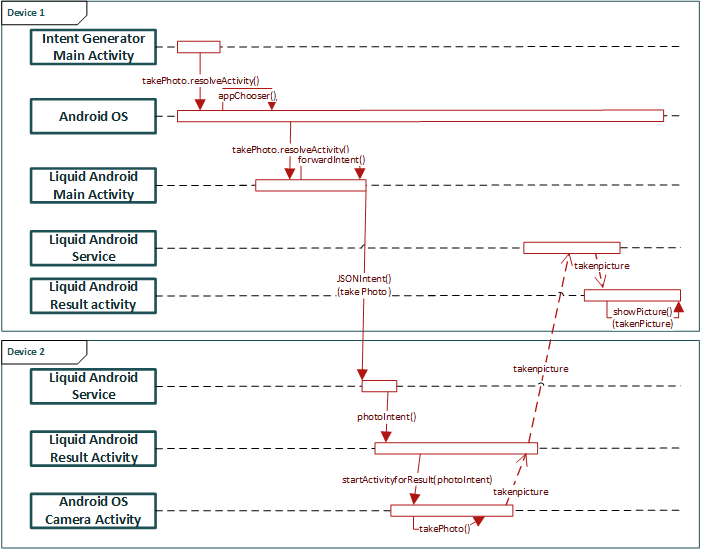
\includegraphics[width=1\textwidth]{sequence2}
	\caption{Live test 2 Sequence Diagram}
	\label{fig:5.8}
\end{figure}\\
As already done with the previous live test case, I want to provide a set of screenshots showing the application behavior while running this example.\\
In \figurename~\ref{fig:5.9} there is the complete flow of actions presented with some real screenshots of the applications I have developed. In particular the screens from \textit{a} to \textit{c} are taken from the first device I have used, a Huawei P9, to generate and forward the so called photo intent.\\
\begin{figure}[h!]
	\centering
	\begin{minipage}{.24\textwidth}\centering
		\subfloat[Send Email\label{subfig-1:intentg2}]{%
			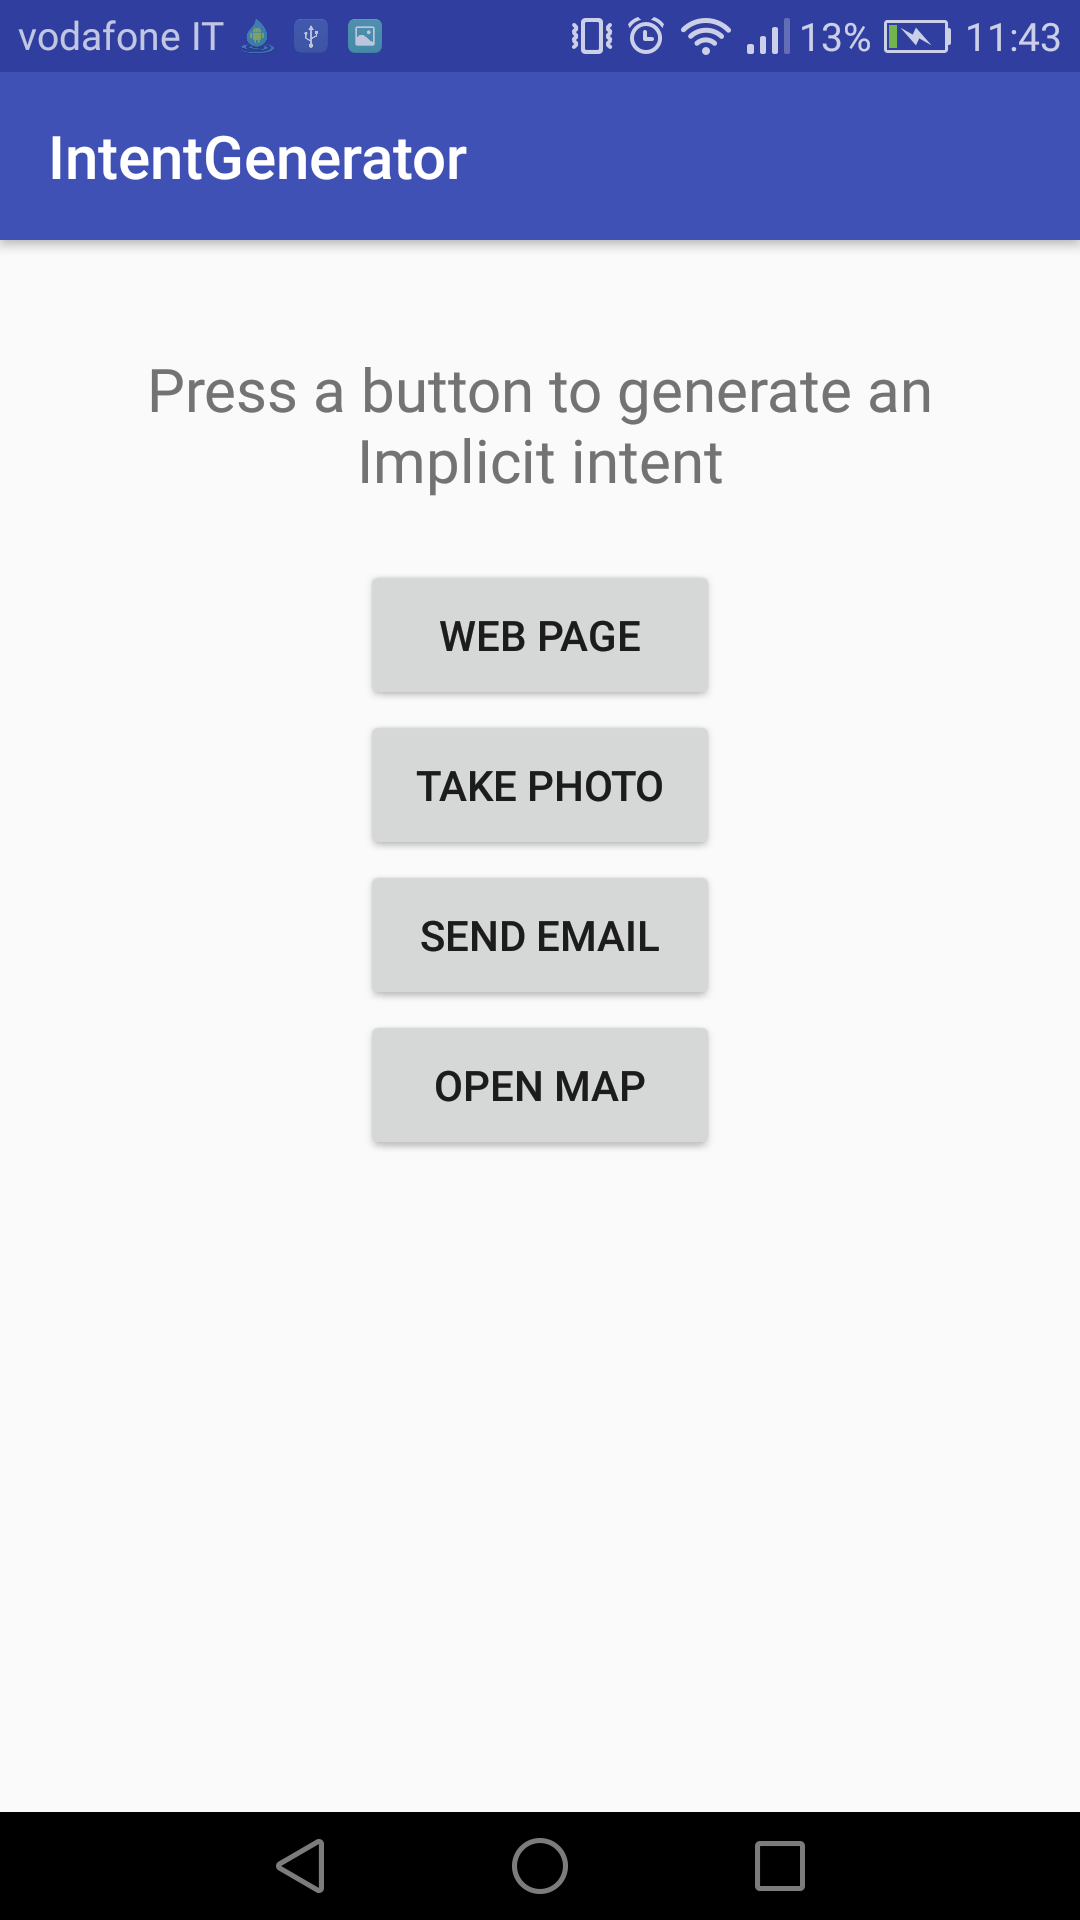
\includegraphics[width=0.9\textwidth]{intentgenerator}
		}
	\end{minipage}
	\begin{minipage}{.24\textwidth}\centering
		\subfloat[App Chooser\label{subfig-2:chooser2}]{%
			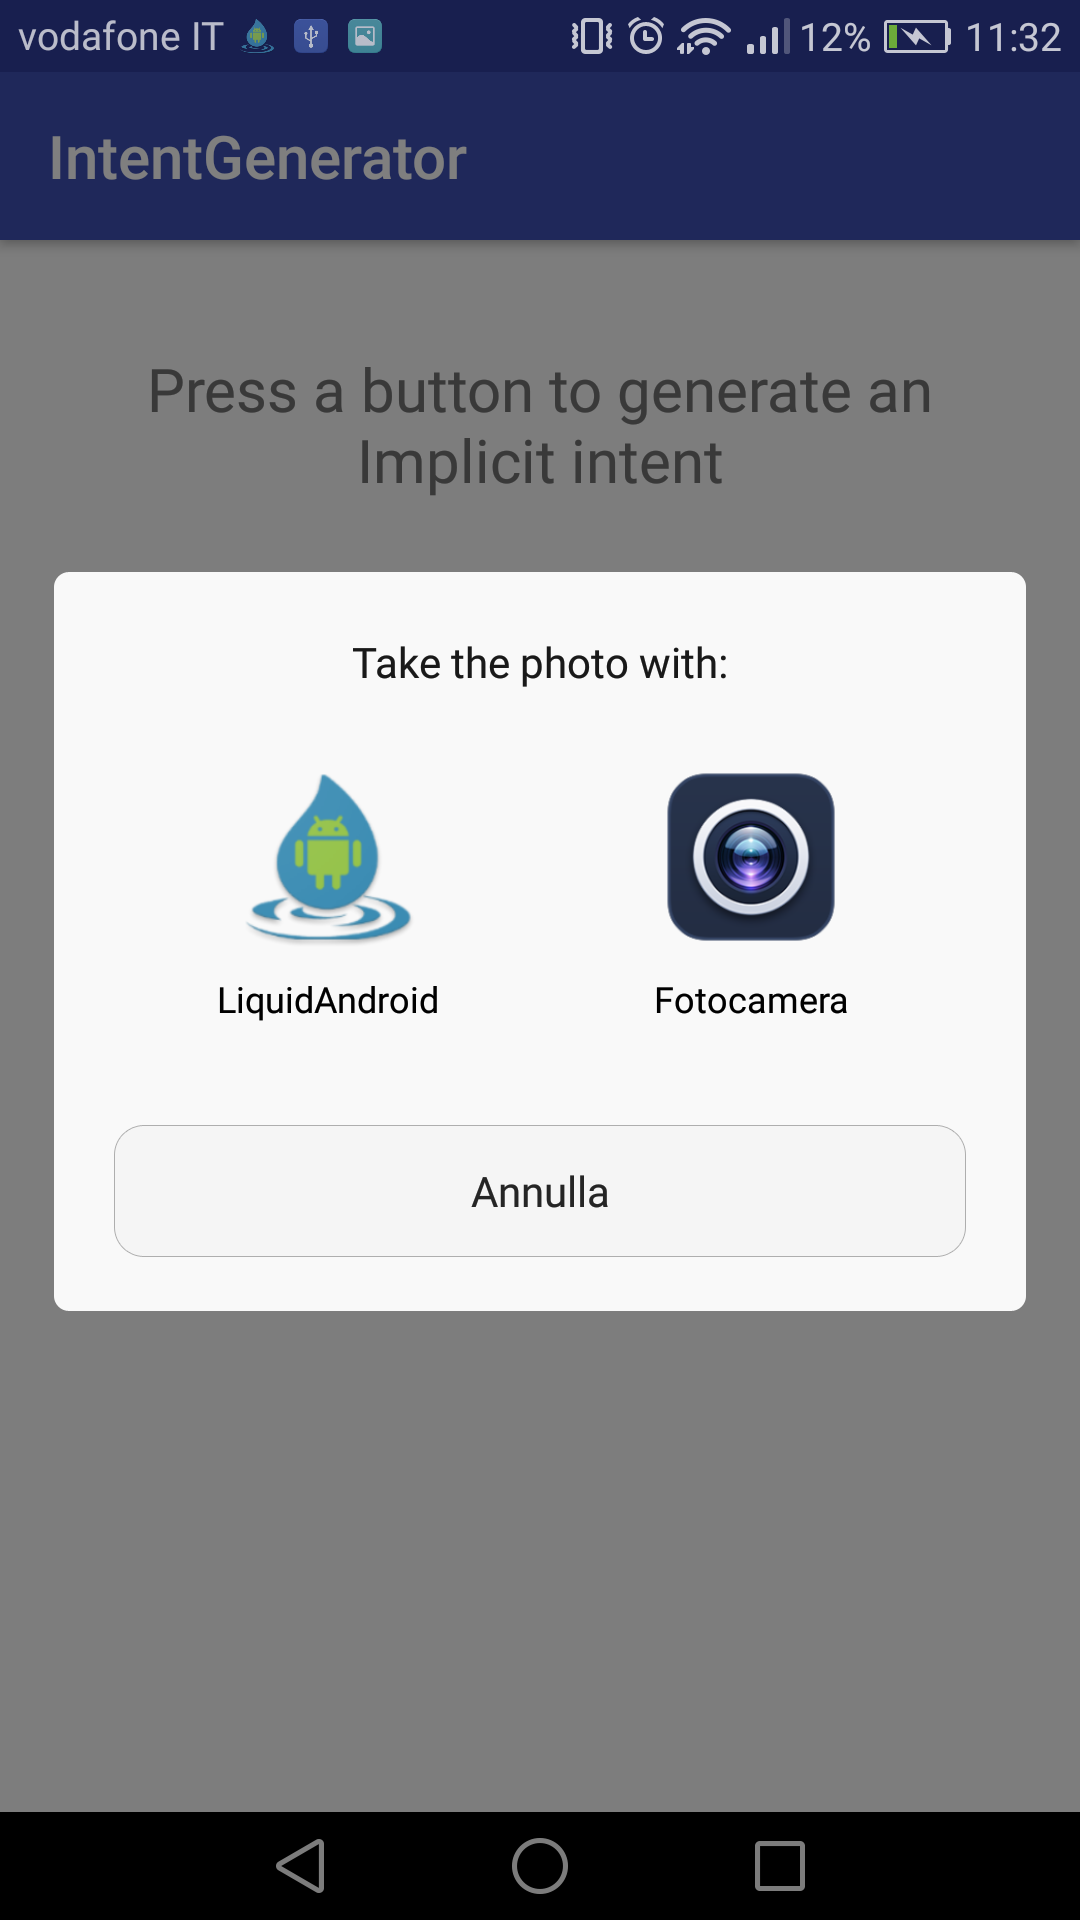
\includegraphics[width=0.9\textwidth]{photochooser}
		}
	\end{minipage}
	\centering
	\begin{minipage}{.24\textwidth}\centering
		\subfloat[Forward Dialog\label{subfig-3:liquid2}]{%
			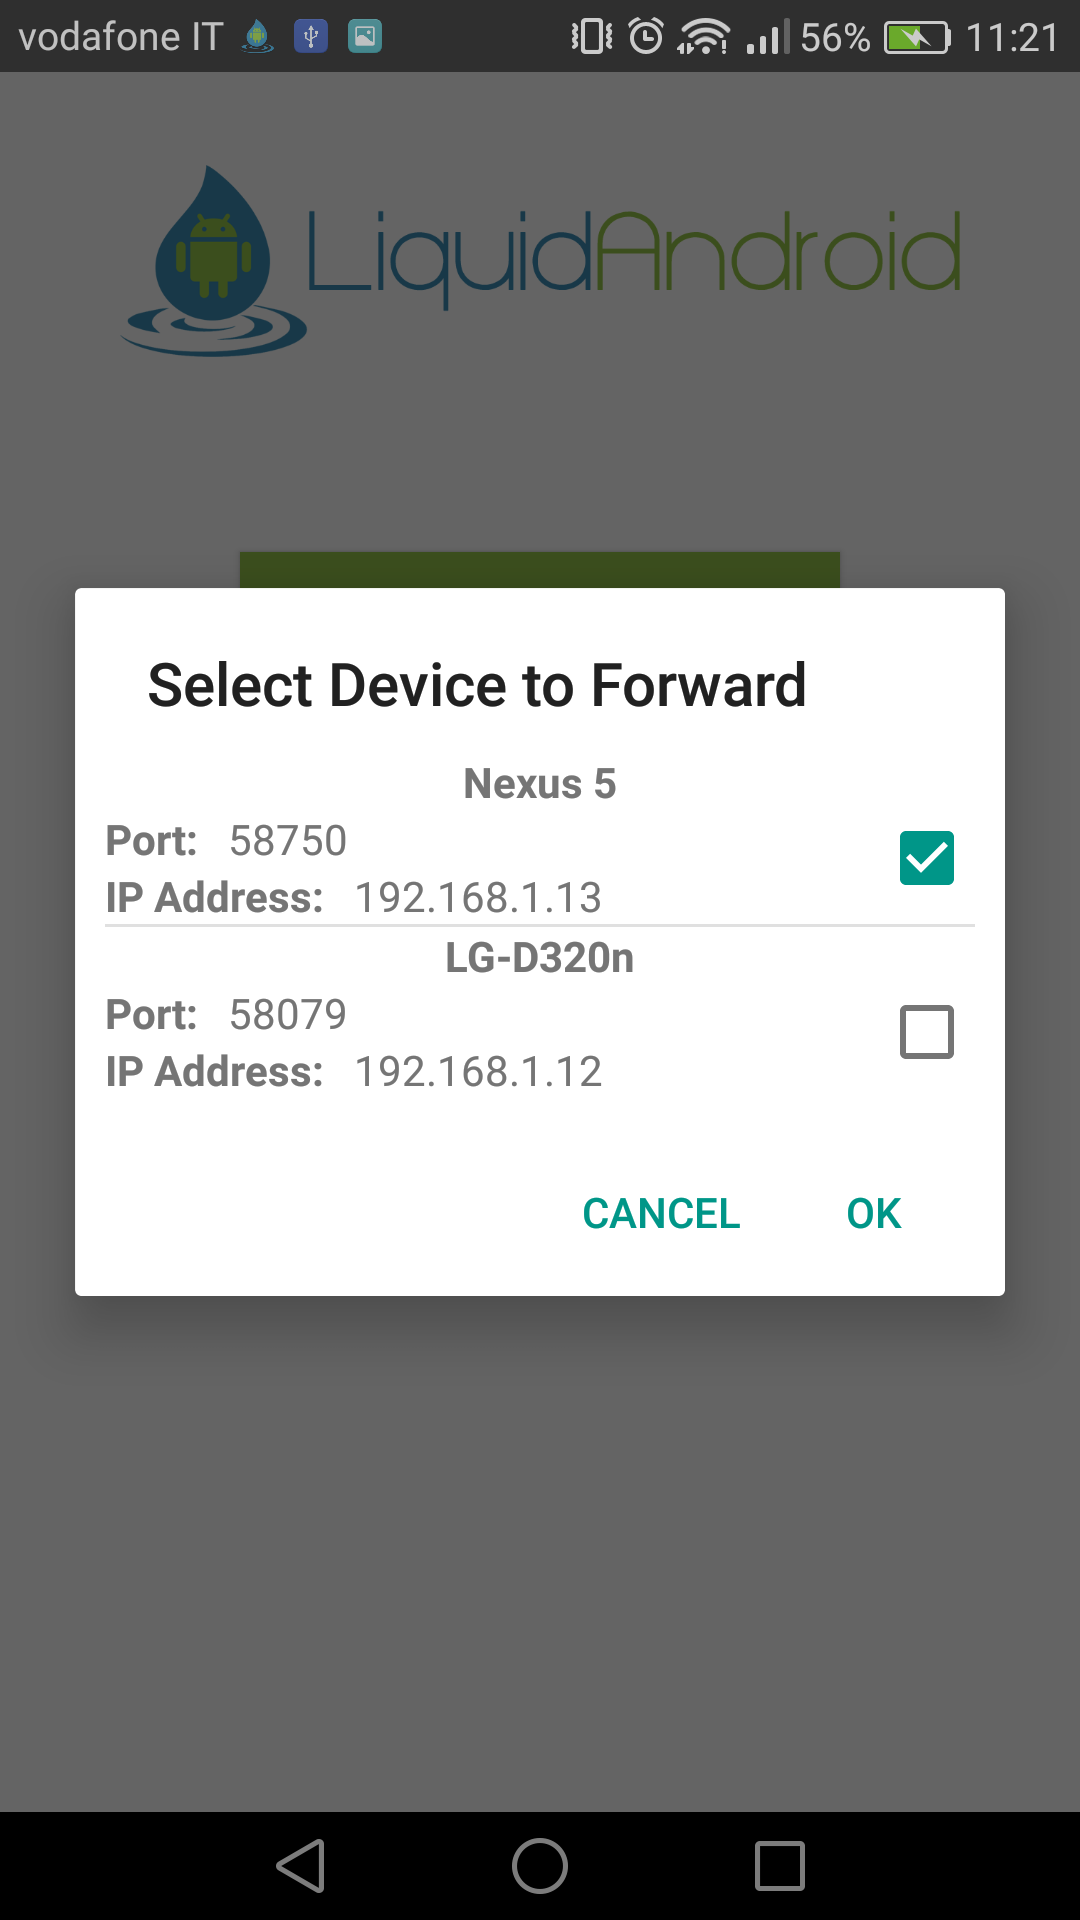
\includegraphics[width=0.9\textwidth]{alert}
		}
	\end{minipage}
	\begin{minipage}{.24\textwidth}\centering
		\subfloat[App Chooser\label{subfig-4:chooser3}]{%
			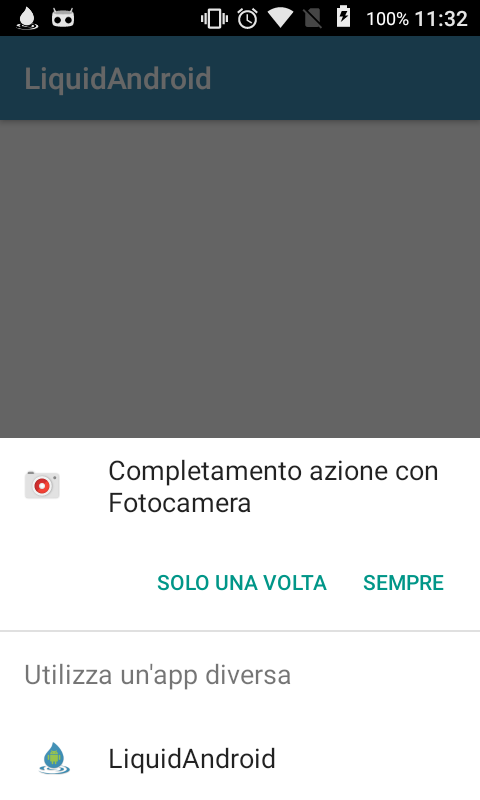
\includegraphics[width=0.9\textwidth]{chosphoto2}
		}
	\end{minipage}
	\phantomcaption
	\label{fig:5.9}
\end{figure}
\begin{figure}[h!]
	\ContinuedFloat
	\centering
	\begin{minipage}{.24\textwidth}\centering
		\bigskip
		\subfloat[Android Camera\label{subfig-5:camera2}]{%
			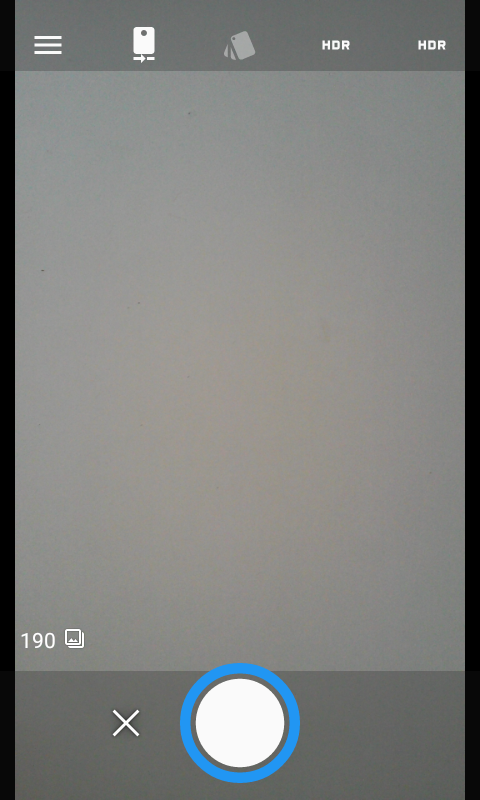
\includegraphics[width=0.9\textwidth]{camera2}
		}
	\end{minipage}
	\begin{minipage}{.24\textwidth}\centering
		\bigskip
		\subfloat[App Chooser\label{subfig-6:chooser2}]{%
			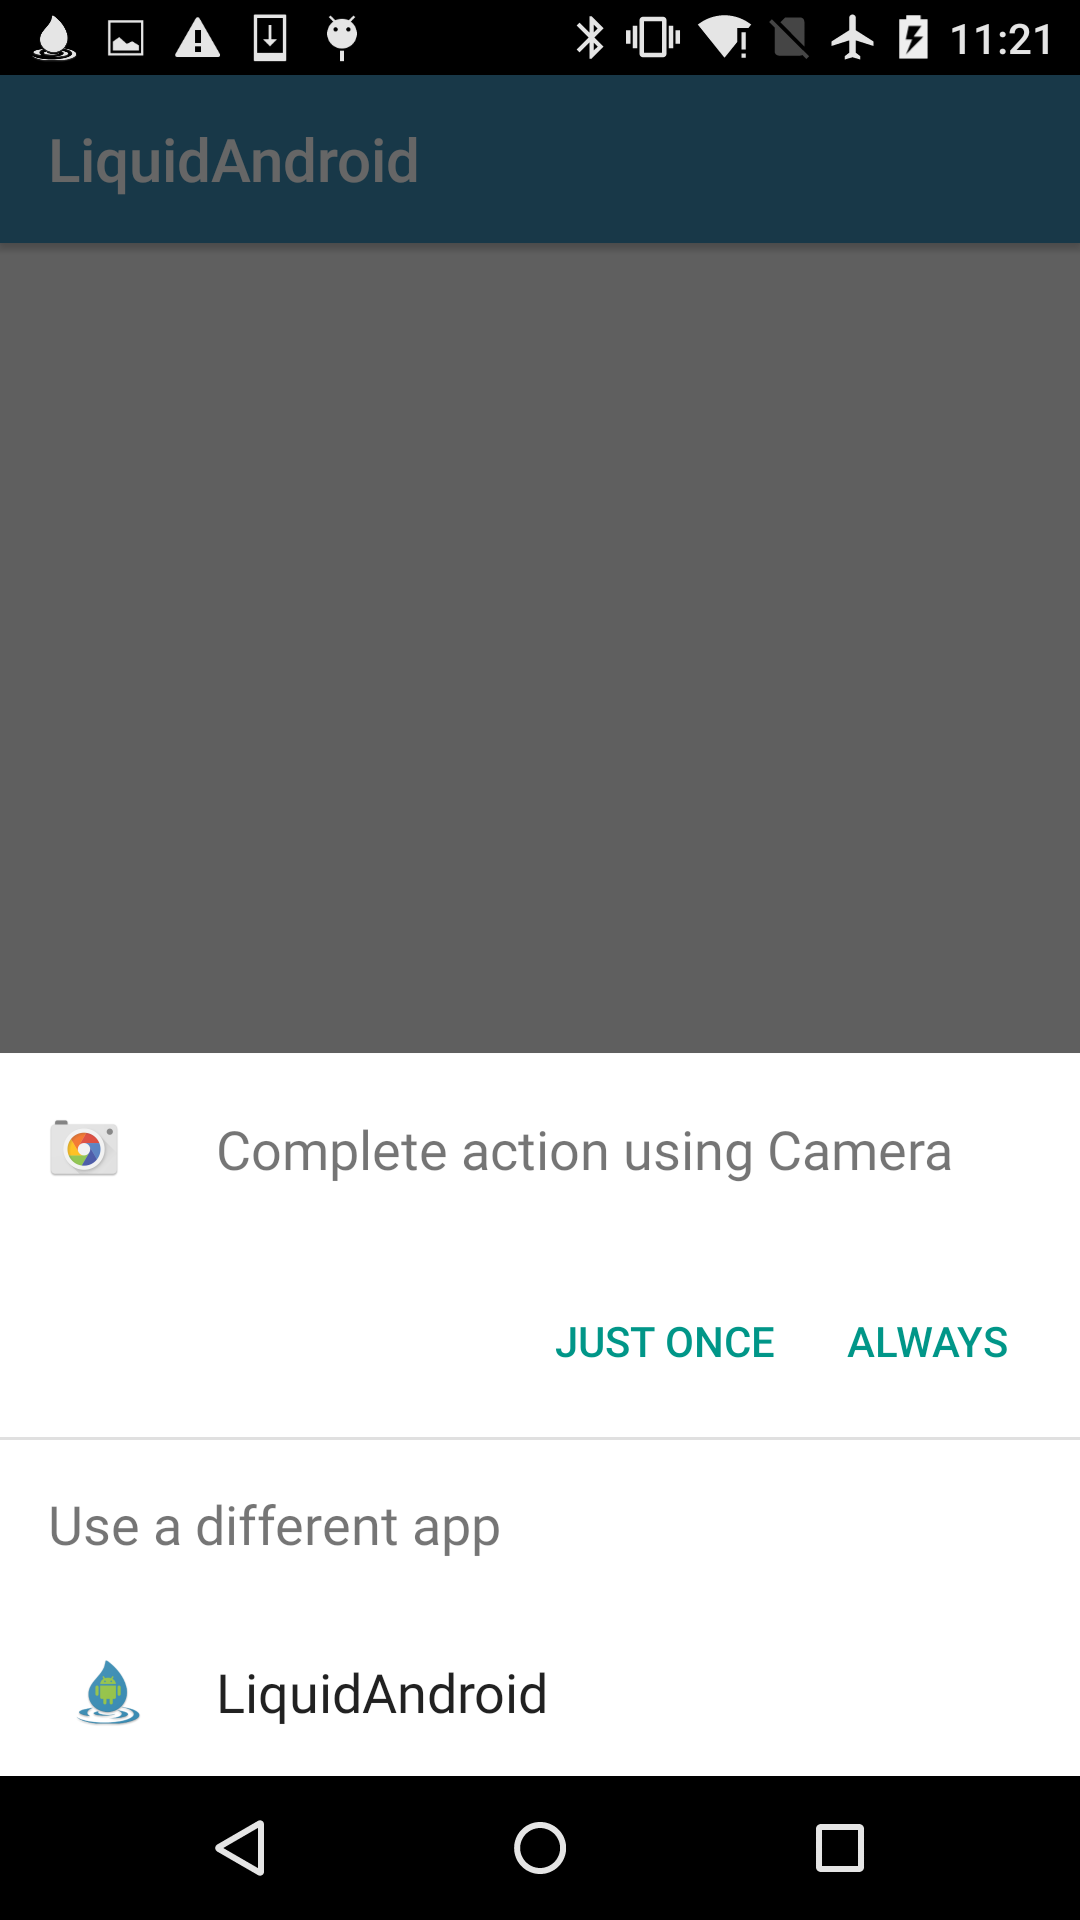
\includegraphics[width=0.9\textwidth]{chosephoto3}
		}
	\end{minipage}
	\begin{minipage}{.24\textwidth}\centering
		\bigskip
		\subfloat[Android Camera\label{subfig-7:camera2}]{%
			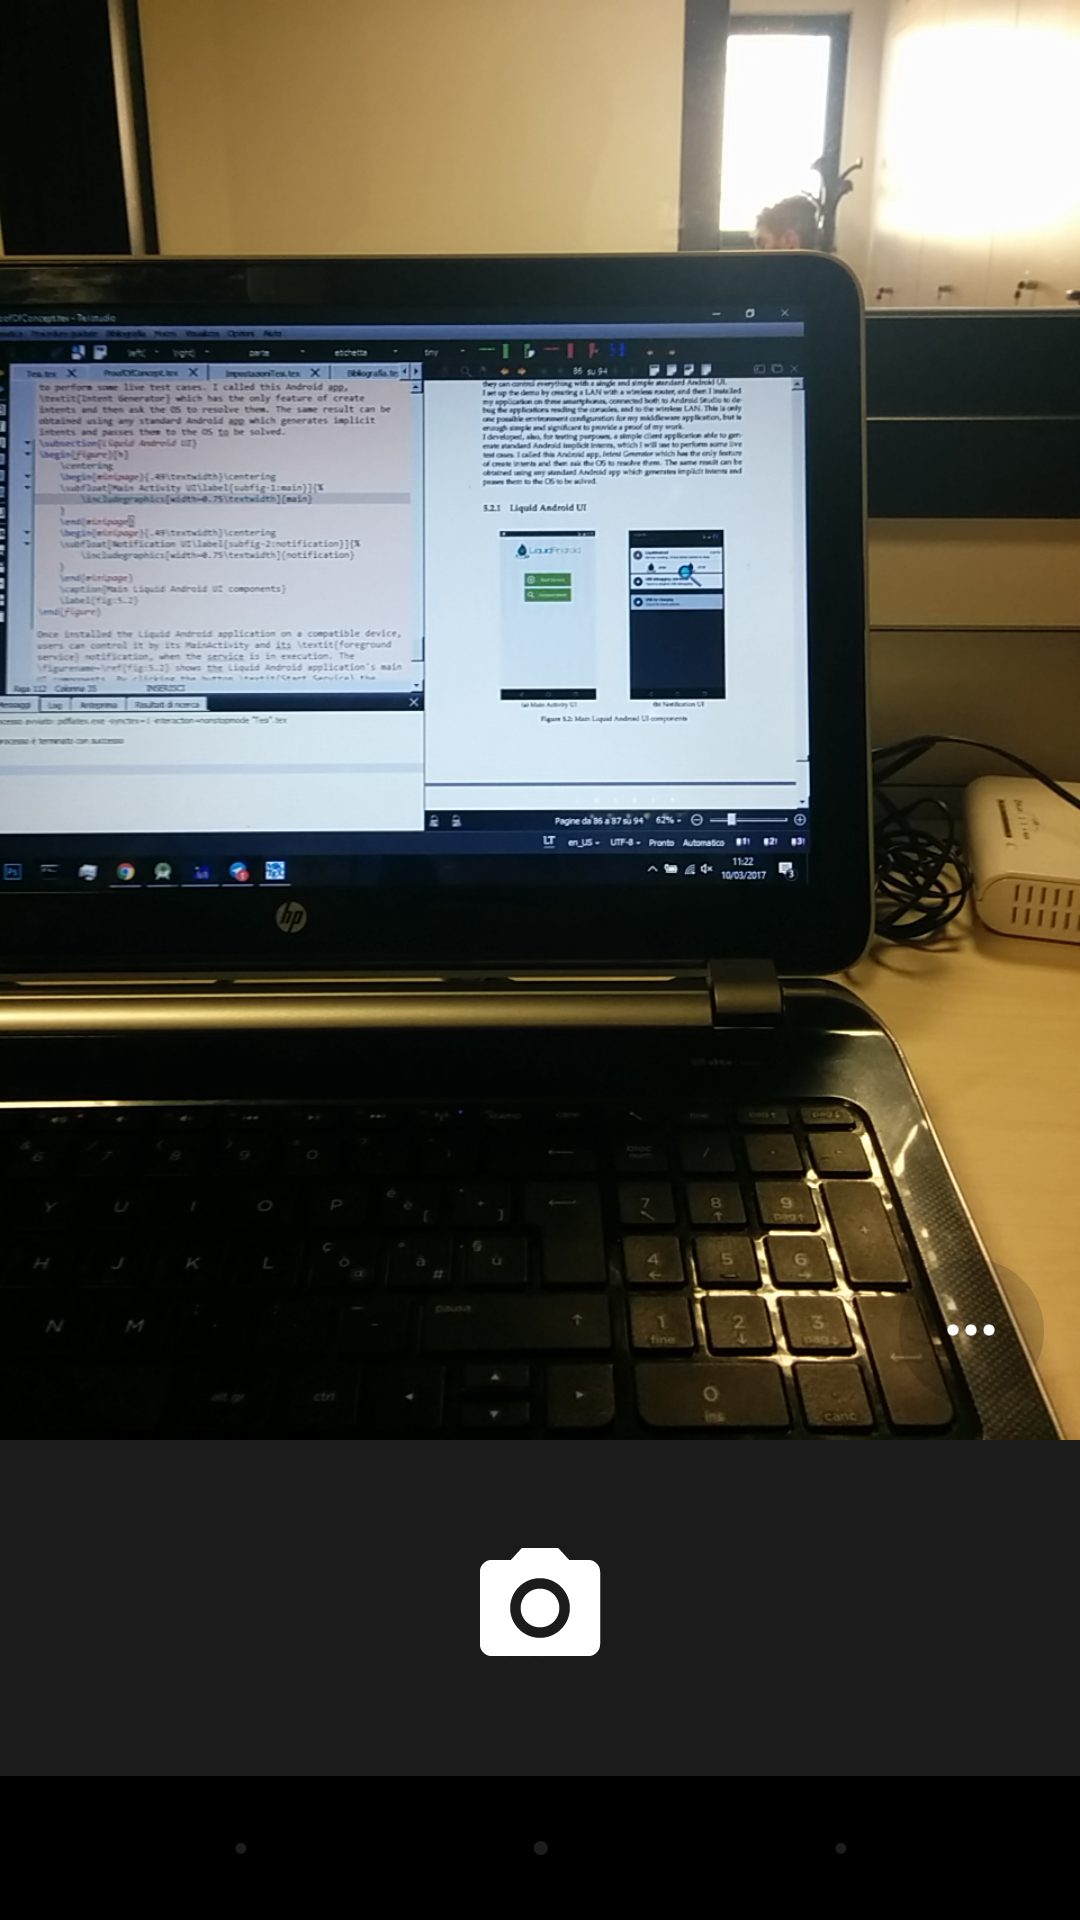
\includegraphics[width=0.9\textwidth]{camera1}
		}
	\end{minipage}
	\begin{minipage}{.24\textwidth}\centering
		\bigskip
		\subfloat[Result Activity\label{subfig-8:chooser2}]{%
			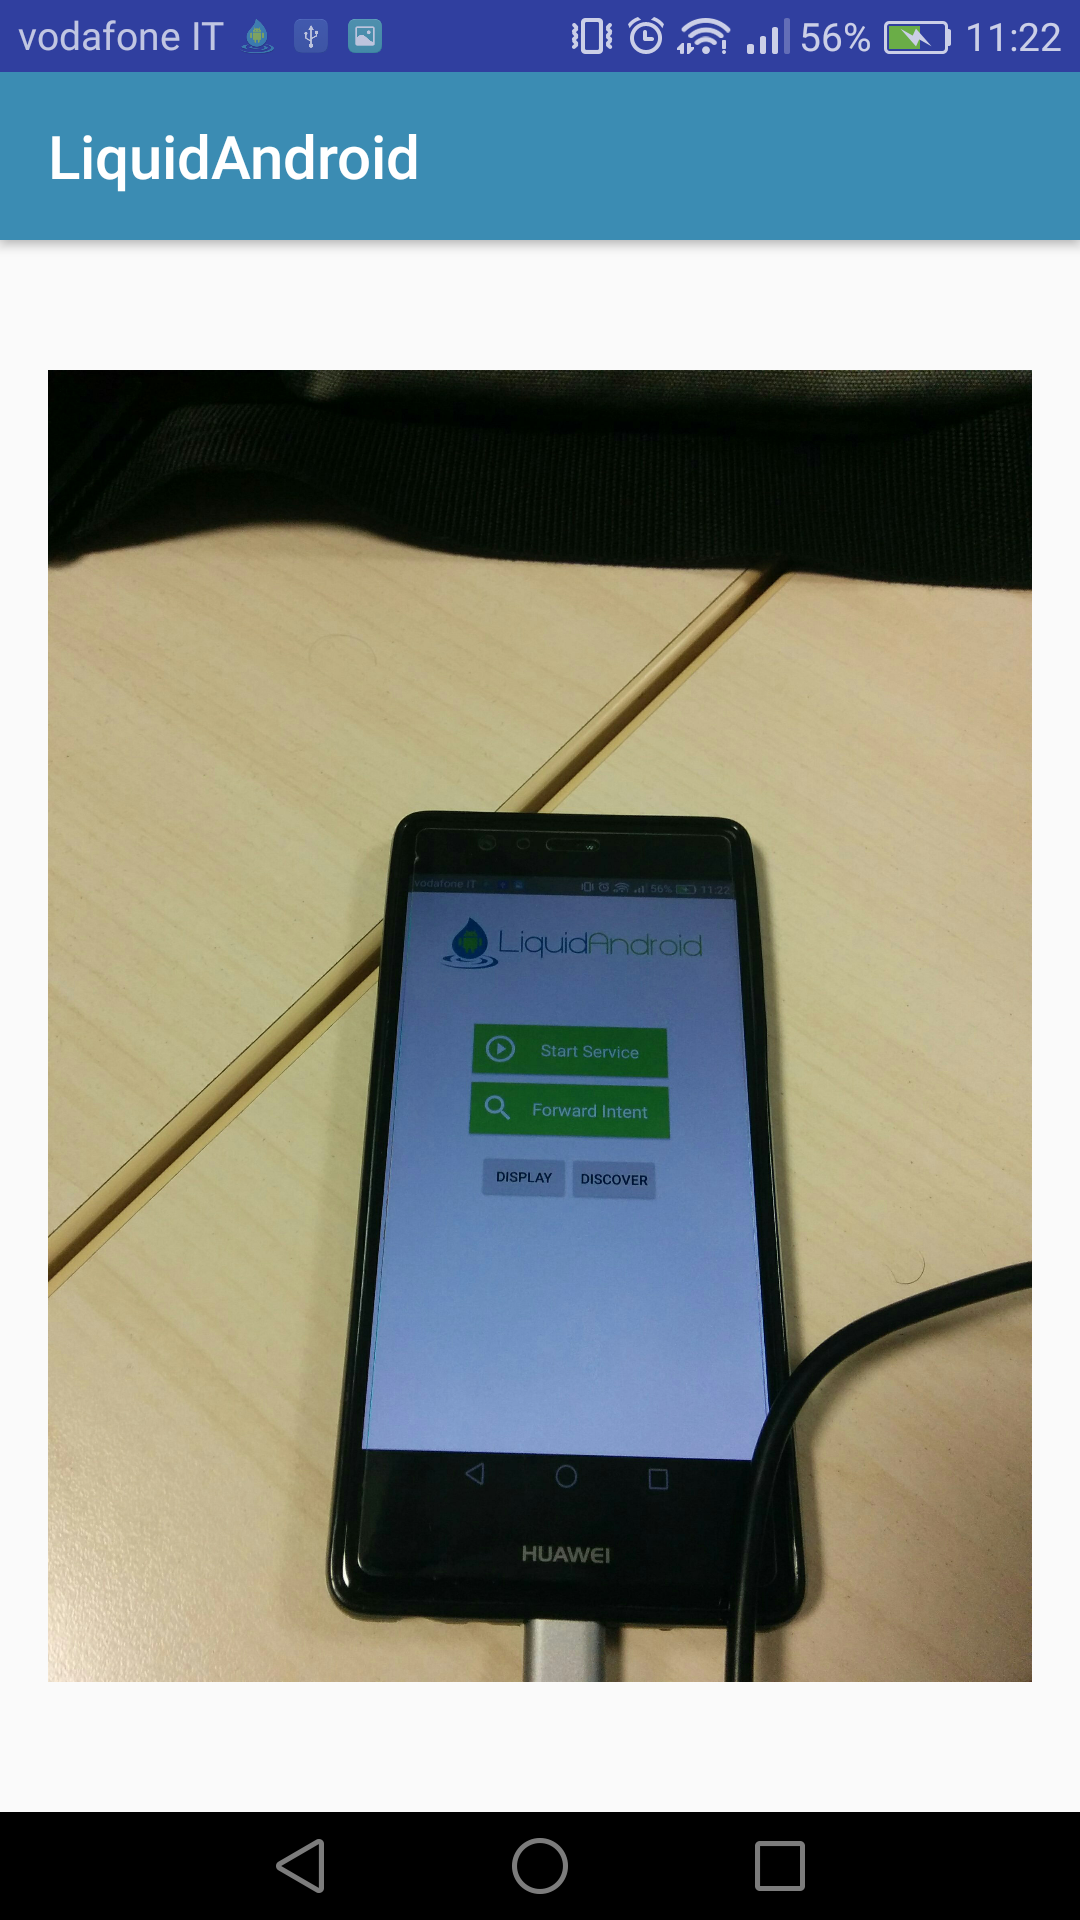
\includegraphics[width=0.9\textwidth]{received1}
		}
	\end{minipage}
	\caption{Complete photo intent live test screenshots}
	
\end{figure}\\
Screens \textit{d} and \textit{e} are taken from the first target device, a LG L70, used to take the first picture. Screens \textit{f} and \textit{g} are taken instead, from the second target device, a Google Nexus 5, used to take the second picture. In the end screen \textit{h} is taken again from the first device, showing the picture taken. All the pictures taken while performing this test, are saved locally on the local storage of the devices which have actually taken the picture, moreover they are saved in the local data storage of the caller device, and are accessible form its gallery application.
\\\\\\
\par This section exhausts the topic, the next chapter deals with the conclusions which can be drawn from my thesis and any future work which can be done to extend and make the work as complete as possible.
%
% ------------------------------------------------------------------------ %
% !TEX encoding = UTF-8 Unicode
% !TEX TS-program = pdflatex
% !TEX root = ../Tesi.tex
% !TeX spellcheck = en_US
% ------------------------------------------------------------------------ %
%
% ------------------------------------------------------------------------ %
% 	CONCLUSIONS AND FUTURE WORKS
% ------------------------------------------------------------------------ %
%
\chapter{Conclusions and Future Work}
%
\label{cap:conclusions}
%
% ------------------------------------------------------------------------ %
%
This chapter aims to analyze what has been done in order to give feedback
and understand if the initial objectives have been reached.\\
The chapter is divided into two parts, the first is the conclusion of the work, with
the analysis of what I have reached with my idea and my implementation; the
second part is focused on future implementation.
\section{Conclusions}
Liquid Android middleware aims to enrich the Android OS functionalities by transforming it in to a fully working distributed operating system. My work aims to differentiate itself from existing commercial solutions, seen at the end of the Chapter \ref{cap:statoarte}, in Section \ref{existings} offering a both low cost and easy to deploy solution using a distributed approaches where mobile devices are actors and computing nodes.\\
Liquid Android middleware offers:
\begin{itemize}
	\item automatic network construction and maintenance, when devices are connected in LAN,
	\item same intent resolution mechanism of the standard Android OS,
	\item intent conversion language and automatic tools to perform the conversions,
	\item same standard Android security mechanisms,
	\item development API, easy to use and to be extended to create other purposes distributed systems.
\end{itemize}
Theoretically speaking the goal was reached: having created the networking structure and having defined a new language suitable for the purpose to distribute intents over the network. In this way the Android OS become a distributed OS over a LAN, because any task which can be done by creating implicit intent can be encapsulated in a message and sent, to be executed, on any device with the service active in the network.The research part
was the study and the definition of mechanisms able to let communicate different devices, using a standard mobile operating system. I have defined the steps needed to perform this kind of extension with any existing mobile operating system. My steps, in \ref{cap:proposedsolution} can be used indeed to create similar solutions for other kind of devices. The creation of the middleware and of reliable connections was more part of the implementation, where I did not introduce innovations in the used technologies. That is because reliable and powerful technologies assure the right behavior of the whole architecture.\\
Tests performed in this work aimed to stress the whole system simulating a common scenario with a few number of devices involved: they shown good overall performance of the framework and its well behavior in terms of scalability and dynamicity. Real Android devices behaved as expected under test conditions and the test app built on purpose was always fully usable.\\
I think the work which has been done is positive, interesting and promising: the
idea of having distributed mobile operating system to let users ,use their devices in an environment as they were a single big device, by sending task to any of them connected with my service, is certainly a good feature nowadays in which this kind of devices are becoming more numerous and less expensive. Moreover it is possible to exploit, such a system, to take advantage of the increasing computing capability of mobile devices, and let them cooperate respecting standard OS mechanisms.
\section{Future Work} 
In this section I would like to briefly report and talk about the future developments which can be done on my work, in order to extend and make the framework as complete possible.
My thesis aims to find a unequivocal and uniform way to extend mobile operating system to give them distributed system functionalities. In particular I want to let any kind of device in a network cooperate with each other to perform task. Obviously It was not possible for
reason of time, and complexity to develop a system to be put on the market nowadays, compatible with all the devices. Thus I selected Android devices because they are the most common, cheap, and they use an open source OS. My work can be part of a more complex and complete architecture which can be widely adopted. Following the the very same steps I have done, it would be possible to define a standard language definition to let any mobile devices communicate and cooperate under the same LAN. My JSON solution can be extended and easily used to adapt also IOS and Windows Phone similar intent mechanism, to reach the global goal.
% todo da sistemare



%
% -----------------------------END------------------------------------- %
%
% ------------------------------------------------------------------------ %
% 	BACKMATTER
% ------------------------------------------------------------------------ %
%
\cleardoublepage
%
\backmatter
%
% ------------------------------------------------------------------------ %
% !TEX encoding = UTF-8 Unicode
% !TEX TS-program = pdflatex
% !TEX root = ../Tesi.tex
% !TEX spellcheck = it-IT
% ------------------------------------------------------------------------ %
%
% ------------------------------------------------------------------------ %
% 	FIGURES COPYRIGHT
% ------------------------------------------------------------------------ %
%
\chapter{Figures Copyright}
%
\label{cap:figurescopyright}
%
% ------------------------------------------------------------------------ %
%
\section*{Chapter 2: State of Art}
\begin{itemize}

	\item Figures \ref{2.1:Categoriesofsmartobjects}, \ref{2.7:iotvswotprotocols}, \ref{2.8:iotvswotobjs}, \ref{2.10:newdivision} and \ref{2.11:foursublayers} are taken from \cite{guinard2011web} and reproduced with the kind authorization of the author, citing his personal website \url{http://dom.guinard.org}.
	
	\item Figures \ref{2.3:Rangeofdifferentnetworks} and \ref{2.5:bigdata5v} are reproduced with the kind authorization of DEIB, my department in Politecnico di Milano and its professors.
	
	\item Figure \ref{2.4:IPv4vsIPv6addresses} is a composition of two different images. Left part is subject to a public domain license. The license notice is available at \url{https://commons.wikimedia.org/wiki/File:Ipv4_address.svg}, which allows the reuse. Right part is subject to a public domain license. The license notice is available at \url{https://commons.wikimedia.org/wiki/File:Ipv6_address.svg}, which allows the reuse.
			
	\item Figure \ref{2.9:flyport} is taken and reproduced with the kind authorization of OpenPicus, \url{www.openpicus.com}.
	
\end{itemize}


\section*{Chapter 4: Solution}
\begin{itemize}

	\item Figure \ref{4.1: hap} are taken from the Apple WWDC 2014 informative pdf \url{http://devstreaming.apple.com/videos/wwdc/2014/701xx8n8ca3aq4j/701/701_designing_accessories_for_ios_and_os_x.pdf}, and according to \url{http://www.apple.com/legal/internet-services/terms/site.html} "Content" section, there is the possibility to reproduce the content, following the 4 points there listed.
	
	\item Figure \ref{4.4:semanticWeb} is subject to a public domain license. The license notice is available at \url{https://commons.wikimedia.org/wiki/File:RDF_example.svg}, which allows the reuse.
	
\end{itemize}
	

%

The images that are not explicitly listed are made by me and no copyright is needed.
 
% -----------------------------END------------------------------------- %
%
% ------------------------------------------------------------------------ %
% !TEX encoding = UTF-8 Unicode
% !TEX TS-program = pdflatex
% !TEX root = ../Tesi.tex
% !TEX spellcheck = it-IT
% ------------------------------------------------------------------------ %
%
% ------------------------------------------------------------------------ %
% 	BIBLIOGRAFIA
% ------------------------------------------------------------------------ %

\cleardoublepage
\nocite{*}	% anche riferimenti non citati
\printbibliography

 % ------------------------------------------------------------------------ %
% ------------------------------------------------------------------------ %
% 	END DOCUMENT
% ------------------------------------------------------------------------ %
%
\end{document}
%
% ------------------------------------------------------------------------ %